% -*- coding: utf-8; -*-
\chapter{Computational Experiments and Analysis}
\label{chap:experiments}
In this chapter, we discuss the computational experiments and the analysis that emerge from them. From now on, all results regarding the proposed algorithm will be identified as HG-means (for Hybrid Genetic K-Means). The results are presented in terms of objective function value and time, and are compared to current state-of-the-art results in the MSSC literature.

The experiments were conducted on an Intel Core i5 2.6 GHz processor machine with 8 GB of RAM memory. The source codes were written in C++, using the UNIX g++ compiler on a Linux Ubuntu 14.04 LTS 64-bit operating system.

Three different analysis are presented in this chapter. The first one analyses the general performance of the proposed algorithm in terms of objective function value and computational time, where we compare our results with the current literature. The second one analyses the impact of instances characteristics, where the objective is to verify if the proposed algorithm is affected by the number of clusters and the size of instances. Finally, we analyse the contribution of crossover and mutation components in the performance of the method.

In the coming result tables, the following notation is used:

\begin{itemize}
	\item $n$ is the size of the instance (number of data points);
	
	\item $m$ is the number of clusters;

	\item $d$ is the number of features;
	
	\item $f_{best}$ is the best known value for the MSSC objective found so far;

	\item $E$ is the error from the best known solution, calculated as:

		\begin{center}
		\large
			$E = \frac{f - f_{best}}{f_{best}} \times 100$
		\end{center}
		
	where $f$ is the value of the MSSC objective found by an algorithm. For HG-means, $E_{med}$ and $E_{avg}$ report the error from the median and average values, respectively;
	
	\item $t$ is the CPU time in seconds;
	
	%\item Bold values are used when HG-means found the new best solution

\end{itemize}

\section{Instances}
\label{sec:instances}
The selection of instances was done in order to cover different types of real data, considering both the instance size and the number of features as important indicators to describe the nature of data. Table \ref{instances} summarizes the characteristics of the adopted instances, which correspond to 24 important benchmarks in recent clustering literature, as reported in \cite{Ordin2014} and \cite{Bagirov2016}. For all considered instances, every feature value is a real or integer number and there is no missing values. The number of data points (instances size) ranges from 59 (smallest) to 434,874 (largest); and the number of features ranges from 2 (smallest) to 128 (largest).

In order to elucidate the coming analysis, we propose the discrimination of these instances according to their sizes, that from now on will by identified as Group A1, Group A2, Group B and Group C of instances.

Groups A1 and A2 correspond to small instances reported in the work of \cite{Ordin2014}. The difference between them is that A1 is composed by really small instances with up to 150 data points, whereas instances in A2 have some hundreds of data points. This distinction is useful to choose a reasonable number of clusters to be tested in each group. For instances A1, tests are performed considering up to 10 clusters, whereas in A2 the number of clusters is extended. Group B of instances correspond to medium/large instances reported also by \cite{Ordin2014}, comprising data where the number of points ranges from 1,060 to 20,000. Group C of instances are the same reported in \cite{Bagirov2016}, where instance sizes ranges from 13,910 to 434,874 data points. This last group is especially relevant as it consider large real world instances, which allows a deeper analysis in the scaling of algorithms.

% -*- coding: utf-8; -*-
\begin{table}[]
\centering
\begin{tabular}{@{}llc@{}}
\toprule
Instance                        & Number of data points & Number of features \\ \midrule
German towns                    & 59                    & 2                  \\
Bavaria postal 1                & 89                    & 3                  \\
Bavaria postal 2                & 89                    & 4                  \\
Fisher’s Iris Plant             & 150                   & 4                  \\
Heart Disease                   & 297                   & 13                 \\
Liver Disorders                 & 345                   & 6                  \\
Ionosphere                      & 351                   & 34                 \\
Congressional Voting Records    & 435                   & 16                 \\
Breast Cancer                   & 683                   & 9                  \\
Pima Indians Diabetes           & 768                   & 8                  \\
TSPLIB1060                      & 1060                  & 2                  \\
Image Segmentation              & 2310                  & 19                 \\
TSPLIB3038                      & 3038                  & 2                  \\
Page Blocks                     & 5473                  & 10                 \\
Pendigit                        & 10992                 & 16                 \\
Gas sensor                      & 13910                 & 128                \\
EEG eye state                   & 14980                 & 14                 \\
D15112                          & 15112                 & 2                  \\
Letters                         & 20000                 & 16                 \\
KEGG metabolic relation network & 53413                 & 20                 \\
Shuttle control                 & 58000                 & 9                  \\
Pla85900                        & 85900                 & 2                  \\
Skin Segmentation               & 245057                & 3                  \\
3D road network                 & 434874                & 3                  \\ \bottomrule
\end{tabular}
\caption{Instances description}
\label{instances}
\end{table}

\section{Parameters calibration}
\label{sec:calibration}
As in most meta-heuristics, the values chosen for parameters directly affect the results. In this work, we consider five main parameters: $w$ (the tournament size for selection), $\mu$ (the population size), $\Pi$ (the maximum size of population), $I_{max}$ (the maximum number of iterations) and $I_S$ (the number of iterations without improvement that causes the algorithm stop). For the parameters related to the management of individuals in the population ($w$, $\mu$ and $\Pi$) we performed a calibration to choose the best configuration for the experiments. For the parameters related to the number of iterations the algorithm takes ($I_{max}$ and $I_S$), we directly set their values to 4000 and 2500, respectively. These values were set in order to obtain results in a time comparable to previous authors.

In preliminary experiments, we started with the following configuration for the free variables, as they produced good and stable results after an initial and manually exploration: $w$ = 3, $\mu$ = 80 and $\Pi$ = 300. From this baseline, we expanded the range of these values by an one-factor-at-a-time (OFAT) approach. Table \ref{calibration} presents the ranges of tested values for each parameter and the final values achieved after increasing/decreasing each parameter value at a time.

% -*- coding: utf-8; -*-
\begin{table}[H]
\centering
\begin{tabular}{@{}lllc@{}}
\toprule
\multicolumn{2}{l}{Parameter}           & Range of values             & Final value \\ \midrule
$w$     & Tournament size for selection & \{2, 3, 4\}                 & 3           \\
$\mu$   & Population size               & \{60, 70, 80, 90, 100\}     & 80          \\
$\Pi$   & Maximum size of population    & \{200, 250, 300, 350, 400\} & 200         \\ \bottomrule
\end{tabular}
\caption{Parameters calibration}
\label{calibration}
\end{table}

We considered a subset of five instances for calibration, that were chosen based on their sizes and number of features (Liver disorders, Ionosphere, Breast cancer, Pima Indians diabetes and TSPLIB1060). Small instances were not considered because in almost all of them the different configurations for calibration achieved the best known result (possibly the global optimal), so they are not so informative. As we consider 3 parameters independently, the combination of parameters resulted in 11 possible configurations, as shown in Table \ref{calibration-results}. For this reason, large instances were also not considered.
%It would take too much time just to calibrate the algorithm, as we run 10 times each experiment.
We chose medium-sized instances and tested 4 different number of clusters (20, 30, 40, 50) for each instance. After measuring the offset between the average error and the execution time for each configuration, we took the best one among the 11 options.

In Table \ref{calibration-results}, the first three columns report the values of parameters $w$, $\mu$ and $\Pi$, whereas the remaining columns report, in turn, the errors from the best, worst, median and average solution, and finally the average time taken to run the considered instances for calibration.

\begin{table}[!h]
\centering
\begin{tabular}{@{}cccccccc@{}}
\toprule
$w$ & $\mu$ & $\Pi$ & $E_{bst}$  & $E_{wst}$ & $E_{med}$ & $E_{avg}$ & Total Time \\ \midrule
3   & 80    & 300   & -4.70      & 0.28      & -0.88     & -1.24     & 940.63     \\
2   & 80    & 300   & -4.83      & 0.27      & -0.81     & -1.25     & 1002.89    \\
4   & 80    & 300   & -4.53      & 0.19      & -0.90     & -1.22     & 854.62     \\
3   & 60    & 300   & -4.86      & 0.34      & -0.93     & -1.21     & 885.68     \\
3   & 70    & 300   & -4.85      & 0.25      & -0.95     & -1.23     & 917.79     \\
3   & 90    & 300   & -4.77      & 0.61      & -0.81     & -1.23     & 957.70     \\
3   & 100   & 300   & -4.80      & 0.34      & -0.73     & -1.23     & 978.47     \\
3   & 80    & 200   & -4.80      & 0.19      & -0.88     & -1.23     & 875.21     \\
3   & 80    & 250   & -4.87      & 0.40      & -0.78     & -1.24     & 1001.25    \\
3   & 80    & 350   & -4.85      & 0.41      & -0.79     & -1.25     & 1017.34    \\
3   & 80    & 400   & -4.91      & 0.32      & -0.76     & -1.26     & 999.21     \\
%2   & 80    & 300   & -4.96      & 0.55      & -0.76     & -1.21     & 960.46     \\
%2   & 60    & 230   & -4.76      & 0.19      & -0.79     & -1.22     & 840.16     \\
%2   & 80    & 300   & -4.92      & 0.70      & -0.72     & -1.18     & 805.58     \\
%2   & 60    & 230   & -4.75      & 0.89      & -0.74     & -1.18     & 804.05     \\
\bottomrule
\end{tabular}
\caption{Results of calibration}
\label{calibration-results}
\end{table}

\section{Experimental results}
\label{sec:results}

\subsection{General performance and computational time}
\label{sec:performance}
The results of numerical experiments regarding solution performance and computational time for groups A1, A2, B and C of instances are presented in Tables \ref{results-all-A1}, \ref{results-all-A2}, \ref{results-all-B} and \ref{results-all-C}, respectively. Due to the stochastic nature of the proposed meta-heuristic, the results of HG-means correspond to the average of 10 runs, where a run is the execution of an instance with a specific $m$. 

For comparison purposes, we analyse the results considering the best known solutions found so far and the results of global K-means (GKM) \cite{Likas2003}, the modified global K-means (MGKM) \cite{Bagirov2008}, the multi-start modified global K-means (MS-MGKM) \cite{Ordin2014} and the difference of convex clustering (DCClust and MS-DCA) \cite{Bagirov2016} algorithms, which are recent works in MSSC literature, corresponding to the state-of-the-art for this problem. For Tables \ref{results-all-A1}, \ref{results-all-A2}, \ref{results-all-B}, the computational time of MS-MGKM, MGKM and GKM algorithms correspond to the measurements performed by an Intel Core 2 Dual 2.50 GHz processor machine with 3 GB of RAM memory, as reported in \cite{Ordin2014}. For Table \ref{results-all-C}, an Intel Core i5 2.90 GHz processor machine with 8 GB of RAM was used to measure DCClust and MS-DCA algorithms, according to \cite{Bagirov2016}.

% HG-means performance analysis
Tables \ref{results-all-A1} and \ref{results-all-A2} presents the results for instances of group A1 and A2. As we can observe, HG-means finds the new best solution or achieves the current best one in all instances for most of $m$ values. In some cases, as in Ionosphere instance, HG-means results reach more than 4\% of the error, a significant improvement. On the other hand, the proposed algorithm requires more computational effort than MS-MGKM, MGKM and GKM algorithms for most of these small instances -- in many cases the computational time of HG-means is similar to MS-MGKM. It is also important to note that in some instances like Bavaria postal 2, Liver disorders, Ionosphere and Pima Indians diabetes, the gap of HG-means results to the best known solutions increases for large $m$.

Table \ref{results-all-B} presents the results for instances of group B. As in results for small instances, HG-means finds the new best solution or achieves the current best one in all instances for most of $m$ values, outperforming MS-MGKM, MGKM and GKM algorithms in terms of solution quality. Regarding computational time, HG-means is faster than MS-MGKM and GKM in TSPLIB3038, faster than MS-MGKM in TSPLIB1060 and has nearly the same time of MS-MGKM and MGKM in Pendigit. For Image segmentation and Page Block -- the latter, only for large $m$ -- HG-means requires more computational effort.

Table \ref{results-all-C} presents the results for instances of group C -- the group with the largest instances. As in the previous results, HG-means finds the new best solution or achieves the current best one in all instances for most of $m$ values. Regarding computational time, HG-means is faster than DCClust for almost all instances, except for EEG eye state and D15112.

{\footnotesize
\centering
\begin{longtable}{@{}llccccccccc@{}}
m  & $f_{best}$ & \multicolumn{2}{c}{MS-MGKM} & \multicolumn{2}{c}{MGKM} & \multicolumn{2}{c}{GKM} & \multicolumn{3}{c}{HGKM}      \\ \midrule
   &            & $E$          & $t$          & $E$         & $t$        & $E$         & $t$       & $E_{med}$ & $E_{avg}$ & $t$   \\
\multicolumn{11}{l}{German towns}                                                                                                  \\
2  & 121430     & 0.00         & 0.00         & 0.00        & 0.00       & 0.00        & 0.00      & 0.00      & 0.00      & 0.07  \\
3  & 77009      & 0.00         & 0.02         & 1.45        & 0.00       & 1.45        & 0.00      & 0.00      & 0.00      & 0.07  \\
4  & 49601      & 0.24         & 0.02         & 0.72        & 0.00       & 0.72        & 0.00      & 0.00      & 0.00      & 0.08  \\
5  & 38716      & 0.00         & 0.02         & 0.00        & 0.00       & 0.00        & 0.00      & 0.00      & 0.00      & 0.08  \\
6  & 30536      & 0.00         & 0.02         & 0.27        & 0.00       & 0.00        & 0.00      & 0.00      & 0.00      & 0.08  \\
7  & 24433      & 0.08         & 0.02         & 0.00        & 0.00       & 0.09        & 0.00      & 0.00      & 0.00      & 0.09  \\
8  & 21631      & 0.00         & 0.02         & 0.54        & 0.00       & 0.64        & 0.00      & -0.68     & -0.68     & 0.10  \\
9  & 18550      & 2.13         & 0.02         & 4.46        & 0.00       & 2.13        & 0.00      & 0.00      & 0.00      & 0.10  \\
10 & 16307      & 1.81         & 0.02         & 1.52        & 0.00       & 1.81        & 0.00      & 0.01      & 0.01      & 0.11  \\
\multicolumn{11}{l}{Bavaria postals 1}                                                                                             \\
2  & 6.0255E+11 & 0.00         & 0.02         & 0.00        & 0.00       & 0.00        & 0.00      & 0.00      & 0.00      & 0.11  \\
3  & 2.9451E+11 & 0.00         & 0.02         & 0.01        & 0.00       & 0.01        & 0.00      & 0.00      & 0.00      & 0.18  \\
4  & 1.0447E+11 & 0.05         & 0.02         & 0.05        & 0.00       & 0.05        & 0.00      & 0.00      & 0.00      & 0.20  \\
5  & 5.9762E+10 & 0.06         & 0.03         & 0.54        & 0.02       & 0.54        & 0.02      & 0.00      & 0.00      & 0.21  \\
6  & 3.5909E+10 & 0.07         & 0.03         & 1.44        & 0.02       & 1.44        & 0.02      & 0.00      & 0.00      & 0.28  \\
7  & 2.1983E+10 & 0.01         & 0.05         & 3.17        & 0.02       & 3.17        & 0.02      & 0.00      & 0.00      & 0.28  \\
8  & 1.3385E+10 & 0.25         & 0.06         & 1.71        & 0.02       & 1.71        & 0.02      & 0.00      & 0.00      & 0.31  \\
9  & 8.4237E+9  & 0.28         & 0.08         & 2.85        & 0.02       & 2.85        & 0.02      & 0.00      & 0.00      & 0.38  \\
10 & 6.4465E+9  & 0.07         & 0.09         & 3.55        & 0.02       & 3.55        & 0.02      & 0.00      & 0.00      & 0.44  \\
\multicolumn{11}{l}{Bavaria postals 2}                                                                                             \\
2  & 4.8631E+10 & 0.00         & 0.00         & 0.00        & 0.00       & 7.75        & 0.00      & 0.00      & 0.00      & 0.07  \\
3  & 1.7399E+10 & 0.00         & 0.00         & 0.00        & 0.00       & 0.00        & 0.00      & 0.00      & 0.00      & 0.08  \\
4  & 7.5591E+9  & 0.00         & 0.00         & 0.00        & 0.00       & 0.00        & 0.00      & 0.00      & 0.00      & 0.09  \\
5  & 5.3429E+9  & 0.00         & 0.00         & 0.00        & 0.00       & 0.00        & 0.00      & 0.00      & 0.00      & 0.10  \\
6  & 3.1876E+9  & 0.00         & 0.00         & 0.00        & 0.00       & 0.00        & 0.00      & 0.00      & 0.00      & 0.11  \\
7  & 2.2159E+9  & 0.61         & 0.00         & 1.50        & 0.02       & 1.50        & 0.00      & -0.04     & -0.04     & 0.13  \\
8  & 1.7045E+9  & 0.00         & 0.02         & 0.00        & 0.02       & 0.00        & 0.00      & 0.00      & 0.00      & 0.13  \\
9  & 1.4030E+9  & 0.00         & 0.02         & 0.00        & 0.02       & 0.00        & 0.00      & -0.14     & -0.14     & 0.14  \\
10 & 1.1841E+9  & 0.00         & 0.02         & 0.00        & 0.02       & 0.00        & 0.00      & -0.26     & -0.26     & 0.15  \\
\multicolumn{11}{l}{Fisher Iris}                                                                                                   \\
2  & 152.348    & 0.00         & 0.00         & 7.32        & 0.00       & 7.32        & 0.00      & 0.00      & 0.00      & 0.08  \\
3  & 78.851     & 0.00         & 0.00         & 0.00        & 0.00       & 0.00        & 0.00      & 0.00      & 0.00      & 0.09  \\
4  & 57.228     & 0.00         & 0.00         & 0.00        & 0.00       & 0.00        & 0.00      & 0.00      & 0.00      & 0.10  \\
5  & 46.446     & 0.00         & 0.00         & 1.86        & 0.00       & 1.86        & 0.00      & 0.00      & 0.00      & 0.12  \\
6  & 39.040     & 0.00         & 0.00         & 1.21        & 0.02       & 1.21        & 0.00      & 0.00      & 0.00      & 0.12  \\
7  & 34.298     & 0.00         & 0.00         & 0.51        & 0.02       & 0.51        & 0.00      & 0.00      & 0.00      & 0.14  \\
8  & 29.989     & 0.18         & 0.02         & 0.73        & 0.02       & 0.73        & 0.00      & 0.00      & 0.00      & 0.16  \\
9  & 27.786     & 1.07         & 0.02         & 0.00        & 0.02       & 0.00        & 0.00      & 0.00      & 0.00      & 0.18  \\
10 & 25.834     & 0.00         & 0.02         & 0.73        & 0.02       & 0.73        & 0.00      & 0.00      & 0.00      & 0.20  \\ \bottomrule
\caption{Objective value and time obtained by algorithms in instances of group A1.}\\
\label{results-all-A1}\\
\end{longtable}}


{\footnotesize
\centering
\begin{longtable}{@{}llccccccccc@{}}
\hline
\multicolumn{1}{l|}{m}  & \multicolumn{1}{l|}{$f_{best}$} & \multicolumn{2}{c|}{MS-MGKM}      & \multicolumn{2}{c|}{MGKM}         & \multicolumn{2}{c|}{GKM}          & \multicolumn{3}{c}{HGKM}      \\ \hline
                        & \multicolumn{1}{l|}{}           & $E$  & \multicolumn{1}{c|}{$t$}   & $E$   & \multicolumn{1}{c|}{$t$}  & $E$   & \multicolumn{1}{c|}{$t$}  & E$_{med}$ & E$_{avg}$ & $t$   \\ \hline
\multicolumn{11}{l}{Heart disease}                                                                                                                                                                    \\ \hline
\multicolumn{1}{l|}{2}  & \multicolumn{1}{l|}{598900}     & 0.00 & \multicolumn{1}{c|}{0.03}  & 93.96 & \multicolumn{1}{c|}{0.00} & 93.96 & \multicolumn{1}{c|}{0.00} & 0.00      & 0.00      & 0.48  \\
\multicolumn{1}{l|}{5}  & \multicolumn{1}{l|}{327970}     & 0.01 & \multicolumn{1}{c|}{0.13}  & 0.08  & \multicolumn{1}{c|}{0.03} & 0.08  & \multicolumn{1}{c|}{0.03} & 0.00      & 0.00      & 1.01  \\
\multicolumn{1}{l|}{10} & \multicolumn{1}{l|}{200650}     & 0.00 & \multicolumn{1}{c|}{0.63}  & 6.96  & \multicolumn{1}{c|}{0.08} & 6.93  & \multicolumn{1}{c|}{0.05} & -0.06     & -0.06     & 1.91  \\
\multicolumn{1}{l|}{15} & \multicolumn{1}{l|}{147650}     & 0.00 & \multicolumn{1}{c|}{1.20}  & 0.06  & \multicolumn{1}{c|}{0.13} & 1.69  & \multicolumn{1}{c|}{0.08} & -0.55     & -0.55     & 2.45  \\
\multicolumn{1}{l|}{20} & \multicolumn{1}{l|}{117780}     & 0.00 & \multicolumn{1}{c|}{1.77}  & 0.77  & \multicolumn{1}{c|}{0.19} & 1.07  & \multicolumn{1}{c|}{0.11} & -0.86     & -0.86     & 3.15  \\
\multicolumn{1}{l|}{25} & \multicolumn{1}{l|}{99292}      & 0.00 & \multicolumn{1}{c|}{2.61}  & 1.74  & \multicolumn{1}{c|}{0.28} & 1.98  & \multicolumn{1}{c|}{0.13} & -0.82     & -0.78     & 3.66  \\
\multicolumn{1}{l|}{30} & \multicolumn{1}{l|}{86216}      & 0.00 & \multicolumn{1}{c|}{3.28}  & 1.36  & \multicolumn{1}{c|}{0.39} & 1.57  & \multicolumn{1}{c|}{0.16} & -0.54     & -0.48     & 4.38  \\
\multicolumn{1}{l|}{40} & \multicolumn{1}{l|}{67701}      & 0.00 & \multicolumn{1}{c|}{4.67}  & 1.05  & \multicolumn{1}{c|}{0.66} & 4.68  & \multicolumn{1}{c|}{0.23} & -1.69     & -1.44     & 5.15  \\
\multicolumn{1}{l|}{50} & \multicolumn{1}{l|}{54878}      & 0.00 & \multicolumn{1}{c|}{6.06}  & 3.33  & \multicolumn{1}{c|}{0.97} & 9.01  & \multicolumn{1}{c|}{0.28} & -1.06     & -1.01     & 6.18  \\ \hline
\multicolumn{11}{l}{Liver disorders}                                                                                                                                                                  \\ \hline
\multicolumn{1}{l|}{2}  & \multicolumn{1}{l|}{423980}     & 0.00 & \multicolumn{1}{c|}{0.08}  & 0.00  & \multicolumn{1}{c|}{0.05} & 0.00  & \multicolumn{1}{c|}{0.03} & 0.00      & 0.00      & 0.27  \\
\multicolumn{1}{l|}{5}  & \multicolumn{1}{l|}{218260}     & 0.06 & \multicolumn{1}{c|}{0.39}  & 0.18  & \multicolumn{1}{c|}{0.13} & 0.07  & \multicolumn{1}{c|}{0.05} & 0.00      & 0.00      & 0.65  \\
\multicolumn{1}{l|}{10} & \multicolumn{1}{l|}{119400}     & 0.00 & \multicolumn{1}{c|}{0.81}  & 0.64  & \multicolumn{1}{c|}{0.27} & 2.38  & \multicolumn{1}{c|}{0.08} & 6.71      & 6.71      & 1.46  \\
\multicolumn{1}{l|}{15} & \multicolumn{1}{l|}{97405}      & 0.00 & \multicolumn{1}{c|}{1.39}  & 0.81  & \multicolumn{1}{c|}{0.42} & 5.16  & \multicolumn{1}{c|}{0.11} & -0.67     & -0.67     & 1.84  \\
\multicolumn{1}{l|}{20} & \multicolumn{1}{l|}{81192}      & 0.00 & \multicolumn{1}{c|}{1.86}  & 1.52  & \multicolumn{1}{c|}{0.77} & 7.33  & \multicolumn{1}{c|}{0.13} & -1.41     & -1.40     & 2.72  \\
\multicolumn{1}{l|}{25} & \multicolumn{1}{l|}{69212}      & 0.00 & \multicolumn{1}{c|}{2.42}  & 0.68  & \multicolumn{1}{c|}{1.39} & 7.49  & \multicolumn{1}{c|}{0.16} & -1.90     & -1.74     & 3.30  \\
\multicolumn{1}{l|}{30} & \multicolumn{1}{l|}{60325}      & 0.00 & \multicolumn{1}{c|}{3.09}  & 0.37  & \multicolumn{1}{c|}{2.20} & 7.77  & \multicolumn{1}{c|}{0.20} & -2.25     & -2.11     & 3.66  \\
\multicolumn{1}{l|}{40} & \multicolumn{1}{l|}{47336}      & 0.87 & \multicolumn{1}{c|}{4.98}  & 0.00  & \multicolumn{1}{c|}{4.77} & 7.82  & \multicolumn{1}{c|}{0.30} & -1.13     & -1.04     & 4.55  \\
\multicolumn{1}{l|}{50} & \multicolumn{1}{l|}{38305}      & 0.28 & \multicolumn{1}{c|}{6.89}  & 0.00  & \multicolumn{1}{c|}{8.39} & 6.63  & \multicolumn{1}{c|}{0.38} & -1.55     & -1.50     & 5.20  \\ \hline
\multicolumn{11}{l}{Ionosphere}                                                                                                                                                                       \\ \hline
\multicolumn{1}{l|}{2}  & \multicolumn{1}{l|}{2419.4}     & 0.00 & \multicolumn{1}{c|}{0.09}  & 0.00  & \multicolumn{1}{c|}{0.06} & 0.00  & \multicolumn{1}{c|}{0.05} & 0.00      & 0.00      & 1.12  \\
\multicolumn{1}{l|}{5}  & \multicolumn{1}{l|}{1891.5}     & 0.00 & \multicolumn{1}{c|}{0.58}  & 1.86  & \multicolumn{1}{c|}{0.17} & 2.28  & \multicolumn{1}{c|}{0.09} & -0.09     & -0.09     & 2.76  \\
\multicolumn{1}{l|}{10} & \multicolumn{1}{l|}{1559.4}     & 0.00 & \multicolumn{1}{c|}{1.06}  & 0.13  & \multicolumn{1}{c|}{0.33} & 0.11  & \multicolumn{1}{c|}{0.17} & -0.60     & -0.58     & 3.97  \\
\multicolumn{1}{l|}{15} & \multicolumn{1}{l|}{1390.1}     & 0.00 & \multicolumn{1}{c|}{1.72}  & 0.92  & \multicolumn{1}{c|}{0.48} & 0.88  & \multicolumn{1}{c|}{0.23} & -2.18     & -2.16     & 5.54  \\
\multicolumn{1}{l|}{20} & \multicolumn{1}{l|}{1252.4}     & 0.00 & \multicolumn{1}{c|}{2.48}  & 1.17  & \multicolumn{1}{c|}{0.66} & 2.99  & \multicolumn{1}{c|}{0.31} & -2.75     & -2.69     & 7.04  \\
\multicolumn{1}{l|}{25} & \multicolumn{1}{l|}{1140.8}     & 0.00 & \multicolumn{1}{c|}{3.38}  & 0.31  & \multicolumn{1}{c|}{0.83} & 4.45  & \multicolumn{1}{c|}{0.38} & -3.34     & -3.28     & 8.38  \\
\multicolumn{1}{l|}{30} & \multicolumn{1}{l|}{1043.0}     & 0.00 & \multicolumn{1}{c|}{4.27}  & 1.28  & \multicolumn{1}{c|}{0.98} & 4.75  & \multicolumn{1}{c|}{0.45} & -4.44     & -4.39     & 9.88  \\
\multicolumn{1}{l|}{40} & \multicolumn{1}{l|}{856.6}      & 0.00 & \multicolumn{1}{c|}{5.59}  & 2.36  & \multicolumn{1}{c|}{1.39} & 6.14  & \multicolumn{1}{c|}{0.61} & -3.58     & -3.46     & 13.11 \\
\multicolumn{1}{l|}{50} & \multicolumn{1}{l|}{702.6}      & 0.00 & \multicolumn{1}{c|}{6.75}  & 3.68  & \multicolumn{1}{c|}{1.83} & 8.05  & \multicolumn{1}{c|}{0.77} & -3.72     & -3.51     & 16.79 \\ \hline
\multicolumn{11}{l}{Congressional vote}                                                                                                                                                               \\ \hline
\multicolumn{1}{l|}{2}  & \multicolumn{1}{l|}{1640.9}     & 0.00 & \multicolumn{1}{c|}{0.13}  & 0.00  & \multicolumn{1}{c|}{0.09} & 0.00  & \multicolumn{1}{c|}{0.06} & 0.00      & 0.00      & 0.72  \\
\multicolumn{1}{l|}{5}  & \multicolumn{1}{l|}{1335.8}     & 0.03 & \multicolumn{1}{c|}{0.38}  & 0.14  & \multicolumn{1}{c|}{0.22} & 0.14  & \multicolumn{1}{c|}{0.13} & 0.00      & 0.00      & 2.28  \\
\multicolumn{1}{l|}{10} & \multicolumn{1}{l|}{1123.3}     & 0.00 & \multicolumn{1}{c|}{0.91}  & 1.86  & \multicolumn{1}{c|}{0.41} & 1.86  & \multicolumn{1}{c|}{0.20} & -0.32     & -0.31     & 4.28  \\
\multicolumn{1}{l|}{15} & \multicolumn{1}{l|}{992.07}     & 0.00 & \multicolumn{1}{c|}{1.73}  & 0.36  & \multicolumn{1}{c|}{0.59} & 0.33  & \multicolumn{1}{c|}{0.30} & -0.84     & -0.75     & 5.31  \\
\multicolumn{1}{l|}{20} & \multicolumn{1}{l|}{906.47}     & 0.00 & \multicolumn{1}{c|}{2.98}  & 0.71  & \multicolumn{1}{c|}{0.80} & 0.34  & \multicolumn{1}{c|}{0.39} & -1.51     & -1.47     & 5.62  \\
\multicolumn{1}{l|}{25} & \multicolumn{1}{l|}{839.75}     & 0.00 & \multicolumn{1}{c|}{4.97}  & 0.92  & \multicolumn{1}{c|}{0.98} & 0.37  & \multicolumn{1}{c|}{0.52} & -2.28     & -2.22     & 6.57  \\
\multicolumn{1}{l|}{30} & \multicolumn{1}{l|}{776.77}     & 0.00 & \multicolumn{1}{c|}{8.75}  & 0.98  & \multicolumn{1}{c|}{1.22} & 2.83  & \multicolumn{1}{c|}{0.59} & -1.45     & -1.48     & 6.93  \\
\multicolumn{1}{l|}{40} & \multicolumn{1}{l|}{689.35}     & 0.00 & \multicolumn{1}{c|}{12.61} & 1.81  & \multicolumn{1}{c|}{1.70} & 1.28  & \multicolumn{1}{c|}{0.83} & -2.88     & -2.84     & 8.48  \\
\multicolumn{1}{l|}{50} & \multicolumn{1}{l|}{617.5}      & 0.00 & \multicolumn{1}{c|}{15.17} & 1.73  & \multicolumn{1}{c|}{2.28} & 1.98  & \multicolumn{1}{c|}{1.06} & -3.39     & -3.32     & 10.18 \\ \hline
\multicolumn{11}{l}{Breast cancer}                                                                                                                                                                    \\ \hline
\multicolumn{1}{l|}{2}  & \multicolumn{1}{l|}{19323}      & 0.00 & \multicolumn{1}{c|}{0.05}  & 0.00  & \multicolumn{1}{c|}{0.02} & 0.00  & \multicolumn{1}{c|}{0.02} & 0.00      & 0.00      & 0.58  \\
\multicolumn{1}{l|}{5}  & \multicolumn{1}{l|}{13705}      & 0.00 & \multicolumn{1}{c|}{0.27}  & 0.52  & \multicolumn{1}{c|}{0.05} & 0.52  & \multicolumn{1}{c|}{0.02} & 0.00      & 0.00      & 1.64  \\
\multicolumn{1}{l|}{10} & \multicolumn{1}{l|}{10205}      & 0.00 & \multicolumn{1}{c|}{0.94}  & 2.70  & \multicolumn{1}{c|}{0.09} & 0.75  & \multicolumn{1}{c|}{0.03} & -0.14     & -0.14     & 3.02  \\
\multicolumn{1}{l|}{15} & \multicolumn{1}{l|}{8704.7}     & 0.00 & \multicolumn{1}{c|}{1.47}  & 0.72  & \multicolumn{1}{c|}{0.17} & 0.04  & \multicolumn{1}{c|}{0.06} & -0.80     & -0.74     & 4.74  \\
\multicolumn{1}{l|}{20} & \multicolumn{1}{l|}{7695.2}     & 0.39 & \multicolumn{1}{c|}{1.94}  & 1.34  & \multicolumn{1}{c|}{0.23} & 0.00  & \multicolumn{1}{c|}{0.09} & -1.19     & -1.13     & 6.79  \\
\multicolumn{1}{l|}{25} & \multicolumn{1}{l|}{6946.4}     & 0.00 & \multicolumn{1}{c|}{2.47}  & 2.86  & \multicolumn{1}{c|}{0.33} & 3.35  & \multicolumn{1}{c|}{0.11} & -0.88     & -0.81     & 7.55  \\
\multicolumn{1}{l|}{30} & \multicolumn{1}{l|}{6360.3}     & 0.00 & \multicolumn{1}{c|}{3.08}  & 3.31  & \multicolumn{1}{c|}{0.44} & 2.99  & \multicolumn{1}{c|}{0.14} & -0.40     & -0.32     & 8.79  \\
\multicolumn{1}{l|}{40} & \multicolumn{1}{l|}{5487.8}     & 0.00 & \multicolumn{1}{c|}{4.05}  & 1.39  & \multicolumn{1}{c|}{0.69} & 3.13  & \multicolumn{1}{c|}{0.20} & -0.62     & -0.64     & 9.87  \\
\multicolumn{1}{l|}{50} & \multicolumn{1}{l|}{4812.3}     & 0.00 & \multicolumn{1}{c|}{5.20}  & 1.85  & \multicolumn{1}{c|}{1.03} & 3.95  & \multicolumn{1}{c|}{0.27} & -1.21     & -1.21     & 11.60 \\ \hline
\multicolumn{11}{l}{Pima Indians diabetes}                                                                                                                                                            \\ \hline
\multicolumn{1}{l|}{2}  & \multicolumn{1}{l|}{5.1424E+6}  & 0.00 & \multicolumn{1}{c|}{0.11}  & 0.12  & \multicolumn{1}{c|}{0.03} & 0.12  & \multicolumn{1}{c|}{0.02} & 0.00      & 0.00      & 0.73  \\
\multicolumn{1}{l|}{5}  & \multicolumn{1}{l|}{1.7369E+6}  & 0.00 & \multicolumn{1}{c|}{0.56}  & 1.02  & \multicolumn{1}{c|}{0.11} & 1.02  & \multicolumn{1}{c|}{0.05} & 0.00      & 0.00      & 1.45  \\
\multicolumn{1}{l|}{10} & \multicolumn{1}{l|}{9.3046E+5}  & 0.00 & \multicolumn{1}{c|}{1.50}  & 0.70  & \multicolumn{1}{c|}{0.20} & 2.04  & \multicolumn{1}{c|}{0.08} & -0.01     & -0.01     & 3.47  \\
\multicolumn{1}{l|}{15} & \multicolumn{1}{l|}{6.9499E+5}  & 0.00 & \multicolumn{1}{c|}{2.25}  & 1.87  & \multicolumn{1}{c|}{0.31} & 1.69  & \multicolumn{1}{c|}{0.13} & -0.04     & -0.04     & 6.43  \\
\multicolumn{1}{l|}{20} & \multicolumn{1}{l|}{5.7241E+5}  & 0.00 & \multicolumn{1}{c|}{3.28}  & 0.88  & \multicolumn{1}{c|}{0.44} & 2.29  & \multicolumn{1}{c|}{0.17} & -0.01     & -0.01     & 8.53  \\
\multicolumn{1}{l|}{25} & \multicolumn{1}{l|}{4.8869E+5}  & 0.00 & \multicolumn{1}{c|}{4.36}  & 1.26  & \multicolumn{1}{c|}{0.58} & 3.31  & \multicolumn{1}{c|}{0.22} & -0.08     & -0.08     & 10.16 \\
\multicolumn{1}{l|}{30} & \multicolumn{1}{l|}{4.3219E+5}  & 0.00 & \multicolumn{1}{c|}{5.61}  & 0.69  & \multicolumn{1}{c|}{0.73} & 3.44  & \multicolumn{1}{c|}{0.27} & -0.29     & -0.28     & 11.92 \\
\multicolumn{1}{l|}{40} & \multicolumn{1}{l|}{3.5656E+5}  & 0.00 & \multicolumn{1}{c|}{7.75}  & 0.69  & \multicolumn{1}{c|}{1.16} & 4.03  & \multicolumn{1}{c|}{0.38} & -0.39     & -0.40     & 13.38 \\
\multicolumn{1}{l|}{50} & \multicolumn{1}{l|}{3.0903E+5}  & 0.00 & \multicolumn{1}{c|}{10.19} & 1.14  & \multicolumn{1}{c|}{1.84} & 5.53  & \multicolumn{1}{c|}{0.48} & -0.14     & -0.12     & 17.91 \\ \hline
\caption{Objective value and time obtained by algorithms in instances of group A2.}\\
\label{results-all-A2}\\
\end{longtable}}

{\footnotesize
\centering
\begin{longtable}{@{}llccccccccc@{}}
\hline
\multicolumn{1}{l|}{m}   & \multicolumn{1}{l|}{$f_{best}$} & \multicolumn{2}{c|}{MS-MGKM}        & \multicolumn{2}{c|}{MGKM}           & \multicolumn{2}{c|}{GKM}            & \multicolumn{3}{c}{HGKM}                  \\ \hline
                         & \multicolumn{1}{l|}{}           & $E$  & \multicolumn{1}{c|}{$t$}     & $E$  & \multicolumn{1}{c|}{$t$}     & $E$  & \multicolumn{1}{c|}{$t$}     & $E_{med}$      & $E_{avg}$      & $t$     \\ \hline
\multicolumn{11}{l}{TSPLIB1060}                                                                                                                                                                                          \\ \hline
\multicolumn{1}{l|}{2}   & \multicolumn{1}{l|}{9.8319E+9}  & 0.00 & \multicolumn{1}{c|}{0.06}    & 0.00 & \multicolumn{1}{c|}{0.08}    & 0.00 & \multicolumn{1}{c|}{0.08}    & 0.00           & 0.00           & 0.54    \\
\multicolumn{1}{l|}{10}  & \multicolumn{1}{l|}{1.7548E+9}  & 0.22 & \multicolumn{1}{c|}{1.14}    & 0.05 & \multicolumn{1}{c|}{0.34}    & 0.23 & \multicolumn{1}{c|}{0.36}    & 0.00           & 0.00           & 2.96    \\
\multicolumn{1}{l|}{20}  & \multicolumn{1}{l|}{7.9179E+8}  & 0.14 & \multicolumn{1}{c|}{3.19}    & 1.88 & \multicolumn{1}{c|}{0.66}    & 1.88 & \multicolumn{1}{c|}{0.69}    & 0.00           & 0.00           & 4.52    \\
\multicolumn{1}{l|}{30}  & \multicolumn{1}{l|}{4.8125E+8}  & 0.24 & \multicolumn{1}{c|}{5.39}    & 3.37 & \multicolumn{1}{c|}{0.97}    & 3.34 & \multicolumn{1}{c|}{1.03}    & 0.00           & 0.00           & 5.11    \\
\multicolumn{1}{l|}{40}  & \multicolumn{1}{l|}{3.4342E+8}  & 0.00 & \multicolumn{1}{c|}{8.28}    & 2.82 & \multicolumn{1}{c|}{1.30}    & 4.00 & \multicolumn{1}{c|}{1.38}    & \textbf{-0.60} & \textbf{-0.58} & 6.84    \\
\multicolumn{1}{l|}{50}  & \multicolumn{1}{l|}{2.5551E+8}  & 1.16 & \multicolumn{1}{c|}{10.20}   & 2.53 & \multicolumn{1}{c|}{1.69}    & 3.10 & \multicolumn{1}{c|}{1.73}    & 0.11           & 0.11           & 7.03    \\
\multicolumn{1}{l|}{60}  & \multicolumn{1}{l|}{1.9960E+8}  & 0.00 & \multicolumn{1}{c|}{13.95}   & 2.42 & \multicolumn{1}{c|}{2.06}    & 3.16 & \multicolumn{1}{c|}{2.08}    & \textbf{-1.06} & \textbf{-0.98} & 9.12    \\
\multicolumn{1}{l|}{80}  & \multicolumn{1}{l|}{1.2967E+8}  & 0.00 & \multicolumn{1}{c|}{18.17}   & 4.44 & \multicolumn{1}{c|}{2.89}    & 4.38 & \multicolumn{1}{c|}{2.80}    & \textbf{-0.57} & \textbf{-0.44} & 11.82   \\
\multicolumn{1}{l|}{100} & \multicolumn{1}{l|}{9.7019E+7}  & 0.00 & \multicolumn{1}{c|}{23.61}   & 3.50 & \multicolumn{1}{c|}{3.75}    & 3.60 & \multicolumn{1}{c|}{3.53}    & \textbf{-0.16} & \textbf{-0.13} & 15.08   \\ \hline
\multicolumn{11}{l}{Image segmentation}                                                                                                                                                                                  \\ \hline
\multicolumn{1}{l|}{2}   & \multicolumn{1}{l|}{3.5606E+7}  & 0.00 & \multicolumn{1}{c|}{0.52}    & 0.00 & \multicolumn{1}{c|}{1.39}    & 0.00 & \multicolumn{1}{c|}{1.06}    & 0.00           & 0.00           & 5.27    \\
\multicolumn{1}{l|}{10}  & \multicolumn{1}{l|}{9.7952E+6}  & 0.64 & \multicolumn{1}{c|}{6.00}    & 1.76 & \multicolumn{1}{c|}{6.75}    & 1.76 & \multicolumn{1}{c|}{3.97}    & 0.00           & 0.00           & 20.41   \\
\multicolumn{1}{l|}{20}  & \multicolumn{1}{l|}{5.1283E+6}  & 0.77 & \multicolumn{1}{c|}{14.41}   & 1.49 & \multicolumn{1}{c|}{13.11}   & 0.09 & \multicolumn{1}{c|}{7.58}    & 0.00           & 0.00           & 37.22   \\
\multicolumn{1}{l|}{30}  & \multicolumn{1}{l|}{3.5074E+6}  & 0.00 & \multicolumn{1}{c|}{27.98}   & 0.07 & \multicolumn{1}{c|}{20.89}   & 0.07 & \multicolumn{1}{c|}{11.36}   & \textbf{-0.01} & \textbf{-0.01} & 45.18   \\
\multicolumn{1}{l|}{40}  & \multicolumn{1}{l|}{2.7398E+6}  & 0.18 & \multicolumn{1}{c|}{46.63}   & 1.24 & \multicolumn{1}{c|}{28.92}   & 1.25 & \multicolumn{1}{c|}{16.67}   & 0.10           & 0.07           & 62.52   \\
\multicolumn{1}{l|}{50}  & \multicolumn{1}{l|}{2.2249E+6}  & 0.55 & \multicolumn{1}{c|}{61.17}   & 2.41 & \multicolumn{1}{c|}{37.72}   & 2.41 & \multicolumn{1}{c|}{18.73}   & \textbf{-0.02} & \textbf{-0.01} & 76.21   \\
\multicolumn{1}{l|}{60}  & \multicolumn{1}{l|}{1.8818E+6}  & 0.00 & \multicolumn{1}{c|}{77.19}   & 2.34 & \multicolumn{1}{c|}{46.91}   & 1.47 & \multicolumn{1}{c|}{22.50}   & \textbf{-0.39} & \textbf{-0.42} & 92.88   \\
\multicolumn{1}{l|}{80}  & \multicolumn{1}{l|}{1.4207E+6}  & 0.00 & \multicolumn{1}{c|}{97.61}   & 1.64 & \multicolumn{1}{c|}{68.81}   & 2.59 & \multicolumn{1}{c|}{30.19}   & \textbf{-0.35} & \textbf{-0.32} & 120.04  \\
\multicolumn{1}{l|}{100} & \multicolumn{1}{l|}{1.1419E+6}  & 0.00 & \multicolumn{1}{c|}{122.92}  & 0.81 & \multicolumn{1}{c|}{93.69}   & 1.74 & \multicolumn{1}{c|}{38.00}   & \textbf{-0.66} & \textbf{-0.63} & 154.15  \\ \hline
\multicolumn{11}{l}{TSPLIB3038}                                                                                                                                                                                          \\ \hline
\multicolumn{1}{l|}{2}   & \multicolumn{1}{l|}{3.1688E+9}  & 0.00 & \multicolumn{1}{c|}{0.56}    & 0.00 & \multicolumn{1}{c|}{0.86}    & 0.00 & \multicolumn{1}{c|}{1.38}    & 0.00           & 0.00           & 1.72    \\
\multicolumn{1}{l|}{10}  & \multicolumn{1}{l|}{5.6025E+8}  & 0.57 & \multicolumn{1}{c|}{4.92}    & 0.58 & \multicolumn{1}{c|}{3.30}    & 2.78 & \multicolumn{1}{c|}{8.41}    & 0.00           & 0.00           & 5.75    \\
\multicolumn{1}{l|}{20}  & \multicolumn{1}{l|}{2.6681E+8}  & 0.20 & \multicolumn{1}{c|}{11.89}   & 0.48 & \multicolumn{1}{c|}{5.77}    & 2.00 & \multicolumn{1}{c|}{16.63}   & 0.00           & 0.00           & 12.31   \\
\multicolumn{1}{l|}{30}  & \multicolumn{1}{l|}{1.7557E+8}  & 0.39 & \multicolumn{1}{c|}{29.17}   & 0.67 & \multicolumn{1}{c|}{8.25}    & 1.45 & \multicolumn{1}{c|}{25.00}   & \textbf{-0.02} & \textbf{-0.02} & 16.02   \\
\multicolumn{1}{l|}{40}  & \multicolumn{1}{l|}{1.2548E+8}  & 0.33 & \multicolumn{1}{c|}{43.59}   & 1.35 & \multicolumn{1}{c|}{10.70}   & 1.35 & \multicolumn{1}{c|}{33.23}   & \textbf{-0.41} & \textbf{-0.41} & 19.49   \\
\multicolumn{1}{l|}{50}  & \multicolumn{1}{l|}{9.8400E+7}  & 0.57 & \multicolumn{1}{c|}{61.75}   & 1.41 & \multicolumn{1}{c|}{13.23}   & 1.19 & \multicolumn{1}{c|}{41.52}   & \textbf{-0.08} & \textbf{-0.09} & 25.92   \\
\multicolumn{1}{l|}{60}  & \multicolumn{1}{l|}{8.1180E+7}  & 0.00 & \multicolumn{1}{c|}{85.42}   & 2.01 & \multicolumn{1}{c|}{15.75}   & 1.02 & \multicolumn{1}{c|}{49.75}   & \textbf{-0.78} & \textbf{-0.77} & 30.85   \\
\multicolumn{1}{l|}{80}  & \multicolumn{1}{l|}{6.0642E+7}  & 0.00 & \multicolumn{1}{c|}{147.11}  & 1.58 & \multicolumn{1}{c|}{20.94}   & 0.95 & \multicolumn{1}{c|}{66.42}   & \textbf{-0.25} & \textbf{-0.22} & 45.54   \\
\multicolumn{1}{l|}{100} & \multicolumn{1}{l|}{4.8182E+7}  & 0.00 & \multicolumn{1}{c|}{211.00}  & 1.52 & \multicolumn{1}{c|}{26.11}   & 2.11 & \multicolumn{1}{c|}{83.16}   & \textbf{-0.86} & \textbf{-0.82} & 56.92   \\ \hline
\multicolumn{11}{l}{Page blocks}                                                                                                                                                                                         \\ \hline
\multicolumn{1}{l|}{2}   & \multicolumn{1}{l|}{5.7937E+10} & 0.00 & \multicolumn{1}{c|}{1.88}    & 0.00 & \multicolumn{1}{c|}{6.92}    & 0.24 & \multicolumn{1}{c|}{8.19}    & 0.00           & 0.00           & 3.84    \\
\multicolumn{1}{l|}{10}  & \multicolumn{1}{l|}{4.5662E+9}  & 0.00 & \multicolumn{1}{c|}{12.08}   & 0.00 & \multicolumn{1}{c|}{34.09}   & 0.80 & \multicolumn{1}{c|}{49.62}   & \textbf{-0.73} & \textbf{-0.73} & 10.46   \\
\multicolumn{1}{l|}{20}  & \multicolumn{1}{l|}{1.6742E+9}  & 0.00 & \multicolumn{1}{c|}{20.75}   & 2.57 & \multicolumn{1}{c|}{62.09}   & 2.37 & \multicolumn{1}{c|}{92.30}   & \textbf{-0.26} & \textbf{-0.25} & 30.50   \\
\multicolumn{1}{l|}{30}  & \multicolumn{1}{l|}{9.3523E+8}  & 0.00 & \multicolumn{1}{c|}{29.83}   & 0.62 & \multicolumn{1}{c|}{89.42}   & 1.38 & \multicolumn{1}{c|}{132.41}  & \textbf{-1.55} & \textbf{-1.55} & 71.93   \\
\multicolumn{1}{l|}{40}  & \multicolumn{1}{l|}{6.2570E+8}  & 0.67 & \multicolumn{1}{c|}{37.14}   & 0.00 & \multicolumn{1}{c|}{118.55}  & 0.17 & \multicolumn{1}{c|}{172.13}  & \textbf{-2.49} & \textbf{-2.41} & 117.52  \\
\multicolumn{1}{l|}{50}  & \multicolumn{1}{l|}{4.2024E+8}  & 0.00 & \multicolumn{1}{c|}{43.42}   & 2.17 & \multicolumn{1}{c|}{149.77}  & 2.21 & \multicolumn{1}{c|}{212.27}  & \textbf{-0.93} & \textbf{-0.92} & 168.89  \\
\multicolumn{1}{l|}{60}  & \multicolumn{1}{l|}{3.0850E+8}  & 0.00 & \multicolumn{1}{c|}{57.25}   & 1.42 & \multicolumn{1}{c|}{184.06}  & 1.09 & \multicolumn{1}{c|}{254.88}  & 0.00           & 0.00           & 233.99  \\
\multicolumn{1}{l|}{80}  & \multicolumn{1}{l|}{2.0436E+8}  & 0.00 & \multicolumn{1}{c|}{90.89}   & 0.69 & \multicolumn{1}{c|}{258.69}  & 2.16 & \multicolumn{1}{c|}{334.36}  & \textbf{-1.33} & \textbf{-1.30} & 427.42  \\
\multicolumn{1}{l|}{100} & \multicolumn{1}{l|}{1.4428E+8}  & 0.00 & \multicolumn{1}{c|}{114.59}  & 0.91 & \multicolumn{1}{c|}{346.94}  & 0.81 & \multicolumn{1}{c|}{415.19}  & \textbf{-0.58} & \textbf{-0.56} & 589.40  \\ \hline
\multicolumn{11}{l}{Pendigit}                                                                                                                                                                                            \\ \hline
\multicolumn{1}{l|}{2}   & \multicolumn{1}{l|}{1.2812E+8}  & 0.00 & \multicolumn{1}{c|}{6.94}    & 0.00 & \multicolumn{1}{c|}{16.73}   & 0.39 & \multicolumn{1}{c|}{9.42}    & 0.00           & 0.00           & 25.58   \\
\multicolumn{1}{l|}{10}  & \multicolumn{1}{l|}{4.9302E+7}  & 0.00 & \multicolumn{1}{c|}{58.58}   & 0.00 & \multicolumn{1}{c|}{137.17}  & 0.00 & \multicolumn{1}{c|}{81.94}   & 0.00           & 0.00           & 71.49   \\
\multicolumn{1}{l|}{20}  & \multicolumn{1}{l|}{3.4123E+7}  & 0.22 & \multicolumn{1}{c|}{144.13}  & 0.39 & \multicolumn{1}{c|}{281.33}  & 0.22 & \multicolumn{1}{c|}{168.36}  & \textbf{-0.30} & \textbf{-0.30} & 182.63  \\
\multicolumn{1}{l|}{30}  & \multicolumn{1}{l|}{2.7157E+7}  & 0.13 & \multicolumn{1}{c|}{254.30}  & 0.00 & \multicolumn{1}{c|}{425.77}  & 0.00 & \multicolumn{1}{c|}{255.52}  & \textbf{-0.25} & \textbf{-0.25} & 305.88  \\
\multicolumn{1}{l|}{40}  & \multicolumn{1}{l|}{2.3446E+7}  & 0.00 & \multicolumn{1}{c|}{387.47}  & 0.00 & \multicolumn{1}{c|}{570.50}  & 0.11 & \multicolumn{1}{c|}{343.11}  & \textbf{-0.03} & \textbf{-0.03} & 490.22  \\
\multicolumn{1}{l|}{50}  & \multicolumn{1}{l|}{2.1090E+7}  & 0.00 & \multicolumn{1}{c|}{523.19}  & 0.20 & \multicolumn{1}{c|}{713.95}  & 0.56 & \multicolumn{1}{c|}{430.71}  & \textbf{-0.18} & \textbf{-0.18} & 671.02  \\
\multicolumn{1}{l|}{60}  & \multicolumn{1}{l|}{1.9357E+7}  & 0.00 & \multicolumn{1}{c|}{678.02}  & 0.36 & \multicolumn{1}{c|}{858.09}  & 0.22 & \multicolumn{1}{c|}{518.97}  & \textbf{-0.21} & \textbf{-0.20} & 823.97  \\
\multicolumn{1}{l|}{80}  & \multicolumn{1}{l|}{1.6961E+7}  & 0.00 & \multicolumn{1}{c|}{1021.52} & 0.11 & \multicolumn{1}{c|}{1148.34} & 0.25 & \multicolumn{1}{c|}{696.94}  & \textbf{-0.48} & \textbf{-0.48} & 1163.43 \\
\multicolumn{1}{l|}{100} & \multicolumn{1}{l|}{1.5258E+7}  & 0.00 & \multicolumn{1}{c|}{1456.25} & 0.35 & \multicolumn{1}{c|}{1438.78} & 0.45 & \multicolumn{1}{c|}{876.94}  & \textbf{-0.18} & \textbf{-0.18} & 1591.32 \\ \hline
\multicolumn{11}{l}{Letter}                                                                                                                                                                                              \\ \hline
\multicolumn{1}{l|}{2}   & \multicolumn{1}{l|}{1.3819E+6}  & 0.00 & \multicolumn{1}{c|}{14.48}   & 0.00 & \multicolumn{1}{c|}{72.89}   & 0.00 & \multicolumn{1}{c|}{40.17}   & 0.00           & 0.00           & 67.89   \\
\multicolumn{1}{l|}{10}  & \multicolumn{1}{l|}{8.5752E+5}  & 0.00 & \multicolumn{1}{c|}{180.42}  & 0.00 & \multicolumn{1}{c|}{583.36}  & 0.00 & \multicolumn{1}{c|}{363.78}  & 0.00           & 0.00           & 423.15  \\
\multicolumn{1}{l|}{20}  & \multicolumn{1}{l|}{6.7263E+5}  & 0.00 & \multicolumn{1}{c|}{463.38}  & 0.53 & \multicolumn{1}{c|}{1202.36} & 0.72 & \multicolumn{1}{c|}{732.23}  & \textbf{-0.01} & \textbf{-0.01} & 819.44  \\
\multicolumn{1}{l|}{30}  & \multicolumn{1}{l|}{5.7977E+5}  & 0.08 & \multicolumn{1}{c|}{741.50}  & 0.00 & \multicolumn{1}{c|}{1811.45} & 0.08 & \multicolumn{1}{c|}{1094.59} & \textbf{-0.19} & \textbf{-0.19} & 1145.33 \\
\multicolumn{1}{l|}{40}  & \multicolumn{1}{l|}{5.1925E+5}  & 0.00 & \multicolumn{1}{c|}{1057.08} & 0.00 & \multicolumn{1}{c|}{2457.58} & 0.78 & \multicolumn{1}{c|}{1453.70} & \textbf{-0.15} & \textbf{-0.15} & 1582.46 \\
\multicolumn{1}{l|}{50}  & \multicolumn{1}{l|}{4.7727E+5}  & 0.00 & \multicolumn{1}{c|}{1384.72} & 0.23 & \multicolumn{1}{c|}{3065.69} & 0.29 & \multicolumn{1}{c|}{1812.06} & \textbf{-0.42} & \textbf{-0.43} & 1880.03 \\
\multicolumn{1}{l|}{60}  & \multicolumn{1}{l|}{4.4166E+5}  & 0.00 & \multicolumn{1}{c|}{1781.64} & 0.12 & \multicolumn{1}{c|}{3678.17} & 0.37 & \multicolumn{1}{c|}{2173.91} & \textbf{-0.24} & \textbf{-0.24} & 2124.35 \\
\multicolumn{1}{l|}{80}  & \multicolumn{1}{l|}{3.9129E+5}  & 0.00 & \multicolumn{1}{c|}{2594.13} & 0.25 & \multicolumn{1}{c|}{4907.64} & 0.64 & \multicolumn{1}{c|}{2892.00} & \textbf{-0.25} & \textbf{-0.25} & 2626.61 \\
\multicolumn{1}{l|}{100} & \multicolumn{1}{l|}{3.5644E+5}  & 0.00 & \multicolumn{1}{c|}{3465.92} & 0.04 & \multicolumn{1}{c|}{6130.53} & 0.29 & \multicolumn{1}{c|}{3611.05} & \textbf{-0.47} & \textbf{-0.46} & 3230.49 \\ \hline
\caption{Objective value and time obtained by algorithms in instances of group B}\\
\label{results-all-B}\\
\end{longtable}}

{\scriptsize
\centering
\begin{longtable}{@{}lclcccccc@{}}
\toprule
Instance          & m  & $f_{best}$       & \multicolumn{5}{c}{E}                       & t         \\ \midrule
                  &    &                  & MS-MGKM & DCClust & MS-DCA & GKM  & GA-KM   & GA-KM     \\
Gas sensor        & 2  & 791185700000000  & 0.00    & 0.00    & 0.00   & 0.00 & -90.00  & 130.42    \\
                  & 3  & 50241200000000   & 0.00    & 0.00    & 0.00   & 0.00 & 0.00    & 164.07    \\
                  & 5  & 32272600000000   & 0.00    & 0.00    & 0.00   & 0.00 & -0.10   & 365.78    \\
                  & 10 & 16552400000000   & 0.00    & 0.00    & 0.00   & 0.00 & -0.18   & 774.47    \\
                  & 12 & 14065500000000   & 0.01    & 0.00    & 0.01   & 0.00 & -0.20   & 903.8     \\
                  & 15 & 11380100000000   & 0.00    & 0.35    & 0.00   & 0.36 & -0.94   & 891.73    \\
                  & 20 & 8791600000000    & 0.00    & 0.62    & 0.16   & 0.62 & -0.21   & 1690.12   \\
                  & 25 & 7234800000000    & 0.00    & 0.47    & 0.00   & 0.16 & -0.28   & 1836.12   \\ \hline
EEG eye state     & 2  & 817813809000     & 0.00    & 0.00    & 0.00   & 0.00 & -4.07   & 15.21     \\
                  & 3  & 183388058000     & 0.00    & 0.00    & 0.00   & 0.00 & 0.00    & 15.45     \\
                  & 5  & 133858000        & 0.00    & 0.00    & 0.00   & 0.00 & 0.00    & 21.1      \\
                  & 10 & 45669000         & 0.00    & 0.00    & 0.00   & 0.00 & -0.80   & 199.53    \\
                  & 12 & 40251000         & 0.00    & 0.01    & 0.00   & 0.00 & -1.43   & 326.09    \\
                  & 15 & 34653000         & 0.05    & 0.26    & 0.05   & 0.00 & 0.00    & 461.9     \\
                  & 20 & 28987000         & 0.00    & 0.96    & 0.03   & 0.00 & -0.01   & 852.61    \\
                  & 25 & 25995000         & 0.12    & 0.00    & 0.12   & 0.63 & -0.18   & 1037.65   \\ \hline
D15112            & 2  & 368403000000     & 0.00    & 0.00    & 0.00   & 0.00 & 0.00    & 12.11     \\
                  & 3  & 253240000000     & 0.00    & 0.00    & 0.00   & 0.00 & 0.00    & 22.35     \\
                  & 5  & 132707000000     & 0.00    & 0.00    & 0.00   & 0.00 & 0.00    & 18.85     \\
                  & 10 & 64892000000      & 0.00    & 0.00    & 0.00   & 0.78 & -0.62   & 55.73     \\
                  & 12 & 54500000000      & 0.01    & 0.00    & 0.92   & 0.02 & 0.00    & 52.11     \\
                  & 15 & 43138000000      & 0.00    & 0.24    & 0.00   & 0.02 & 0.00    & 79.35     \\
                  & 20 & 32177000000      & 0.25    & 0.00    & 0.25   & 0.01 & 0.00    & 88.91     \\
                  & 25 & 25309000000      & 0.00    & 0.00    & 0.00   & 0.49 & -0.04   & 148.71    \\ \hline
KEGG metabolic    & 2  & 1138530000       & 0.00    & 0.00    & 0.00   & 0.00 & 0.00    & 76.24     \\
                  & 3  & 490060000        & 0.00    & 0.00    & 0.00   & 0.00 & 0.00    & 89.49     \\
                  & 5  & 188367000        & 0.00    & 0.00    & 0.00   & 0.00 & 0.00    & 129.56    \\
                  & 10 & 63515000         & 0.00    & 0.09    & 0.00   & 0.00 & -4.73   & 280.43    \\
                  & 12 & 47825000         & 0.00    & 0.49    & 0.41   & 0.00 & -0.95   & 366.41    \\
                  & 15 & 35484000         & 3.28    & 0.01    & 0.00   & 3.28 & -1.54   & 549.13    \\
                  & 20 & 25430000         & 0.00    & 0.47    & 0.29   & 1.26 & -2.83   & 1067.4    \\
                  & 25 & 19289000         & 0.51    & 0.37    & 0.00   & 0.67 & -1.03   & 1598.53   \\ \hline
Shuttle control   & 2  & 2134329000       & 0.00    & 0.00    & 0.00   & 0.00 & 0.00    & 47.3903   \\
                  & 3  & 1085415000       & 0.00    & 0.00    & 0.00   & 0.00 & 0.00    & 50.76263  \\
                  & 5  & 724479000        & 0.00    & 0.28    & 0.01   & 0.00 & 0.00    & 65.71563  \\
                  & 10 & 283216000        & 0.32    & 0.20    & 0.32   & 0.00 & -0.02   & 142.35133 \\
                  & 12 & 214136000        & 0.44    & 4.04    & 0.45   & 0.00 & 0.00    & 184.05285 \\
                  & 15 & 153154000        & 0.00    & 0.72    & 0.01   & 0.00 & 0.00    & 244.10974 \\
                  & 20 & 106012000        & 0.00    & 0.58    & 0.02   & 0.00 & -3.67   & 566.7401  \\
                  & 25 & 78727000         & 1.50    & 0.00    & 1.54   & 1.50 & -3.60   & 996.57    \\ \hline
Pla85900          & 2  & 3749080000000000 & 0.00    & 0.00    & 0.00   & 0.00 & 0.00    & 94.71     \\
                  & 3  & 2280570000000000 & 0.00    & 0.00    & 0.00   & 0.00 & 0.00    & 123.39    \\
                  & 5  & 1339720000000000 & 0.00    & 0.00    & 0.00   & 0.00 & 0.00    & 150.62    \\
                  & 10 & 682940000000000  & 0.00    & 0.00    & 0.00   & 0.00 & 0.00    & 367.64    \\
                  & 12 & 575040000000000  & 0.19    & 0.00    & 0.19   & 0.00 & 0.00    & 451.81    \\
                  & 15 & 462490000000000  & 0.00    & 0.00    & 0.00   & 0.03 & -0.47   & 672.32    \\
                  & 20 & 349880000000000  & 0.00    & 0.52    & 0.00   & 0.29 & -0.02   & 771.41    \\
                  & 25 & 282650000000000  & 0.11    & 0.00    & 0.11   & 0.94 & -0.15   & 1006.62   \\ \hline
Skin segmentation & 2  & 1322360000       & 0.00    & 0.00    & 0.00   & 0.00 & -100.00 &           \\
                  & 3  & 893620000        & 0.00    & 0.00    & 0.00   & 0.00 & -100.00 &           \\
                  & 5  & 502030000        & 0.00    & 0.00    & 0.00   & 0.00 & -100.00 &           \\
                  & 10 & 251220000        & 0.00    & 0.00    & 0.00   & 0.00 & -100.00 &           \\
                  & 12 & 214160000        & 0.55    & 0.00    & 0.55   & 0.00 & -100.00 &           \\
                  & 15 & 169640000        & 0.18    & 0.18    & 0.19   & 0.00 & -100.00 &           \\
                  & 20 & 127700000        & 0.17    & 0.14    & 0.17   & 0.00 & -100.00 &           \\
                  & 25 & 102990000        & 0.00    & 0.00    & 0.00   & 0.00 & -100.00 &           \\ \hline
3D road network   & 2  & 49132980         & 0.00    & 0.00    & 0.00   & 0.00 & -100.00 &           \\
                  & 3  & 22778180         & 0.00    & 0.00    & 0.00   & 0.00 & -100.00 &           \\
                  & 5  & 8825740          & 0.00    & 0.00    & 0.01   & 0.00 & -100.00 &           \\
                  & 10 & 2567100          & -       & 0.00    & 0.21   & -    & -100.00 &           \\
                  & 12 & 1849760          & -       & 0.00    & 0.05   & -    & -100.00 &           \\
                  & 15 & 1270720          & -       & 0.00    & 0.26   & -    & -100.00 &           \\
                  & 20 & 808720           & -       & 0.00    & 0.73   & -    & -100.00 &           \\
                  & 25 & 603340           & -       & 1.93    & 0.00   & -    & -100.00 &         
\\ \bottomrule
\caption{Objective value and time obtained by algorithms in large instances}
\end{longtable}}
\label{results-all-C}

\subsection{Impact of the number of clusters}

From the performance observed in the results of HG-means algorithm in both solution quality and computational time, we sought to verify if the algorithm works well by increasing the number of clusters. %This analysis is very important, since clustering tasks that require more groups are, in general, more difficult tasks, since we are dealing with a larger combinatorial problem.
This analysis is very important to confirm the robustness of the method, since we are dealing with a larger combinatorial problem when $m$ is large.

Table \ref{m-analysis} presents how HG-means performs for different numbers of clusters. For each group of instances, it reports the average error ($E_{avg}$) to the best known solution when varying the number of clusters ($m$). For instances A1, A2 and B, HG-means has the most significant improvements -- compared to the best known solution -- in cases where $m$ is large. For instances of group C, HG-means increased the gap to the best known solution when $m$ = (2, 20, 25), confirming the robustness of the method.

\begin{table}[H]
\centering
\begin{tabular}{@{}lccccccccc@{}}
\hline
Instances A1 &        &       &       &       &       &       &       &       &       \\
$m$          & 2      & 3     & 4     & 5     & 6     & 7     & 8     & 9     & 10    \\
$E_{avg}$    & 0.00   & 0.00  & 0.00  & 0.00  & 0.00  & -0.01 & -0.17 & -0.03 & -0.06 \\ \hline
Instances A2 &        &       &       &       &       &       &       &       &       \\
$m$          & 2      & 5     & 10    & 15    & 20    & 25    & 30    & 40    & 50    \\
$E_{avg}$    & 0.00   & -0.02 & 0.94  & -0.82 & -1.26 & -1.48 & -1.51 & -1.64 & -1.78 \\ \hline
Instances B  &        &       &       &       &       &       &       &       &       \\
$m$          & 2      & 10    & 20    & 30    & 40    & 50    & 60    & 80    & 100   \\
$E_{avg}$    & 0.00   & -0.12 & -0.09 & -0.33 & -0.59 & -0.25 & -0.43 & -0.50 & -0.46 \\ \hline
Instances C  &        &       &       &       &       &       &       &       &       \\
$m$          & 2      & 3     & 5     & 10    & 12    & 15    & 20    & 25    &       \\
$E_{avg}$    & -11.76 & 0.00  & -0.01 & -0.79 & -0.38 & -0.57 & -1.11 & -1.02 &       \\ \hline
\end{tabular}
\caption{HG-means average performance for different numbers of clusters}
\label{m-analysis}
\end{table}



Figures \ref{fig:error-A1} to and \ref{fig:error-C} display the percentage gap of the methods when considering different number of clusters. In these figures, results are shown for each instance, rather than the aggregated values of Table \ref{m-analysis}.

%\begin{figure}[H]
%\centering
%\subfigure[TSPLIB1060]{\label{fig:errorB-a}\includegraphics[width=0.45\textwidth]{img/error-tsplib1060}}
%\subfigure[Image segmentation]{\label{fig:errorB-b}\includegraphics[width=0.45\textwidth]{img/error-image}}
%\subfigure[TSPLIB3038]{\label{fig:errorB-c}\includegraphics[width=0.45\textwidth]{img/error-tsplib3038}}
%\subfigure[Page blocks]{\label{fig:errorB-d}\includegraphics[width=0.45\textwidth]{img/error-page}}
%\subfigure[Pendigit]{\label{fig:errorB-e}\includegraphics[width=0.45\textwidth]{img/error-pendigit}}
%\subfigure[Letter]{\label{fig:errorB-f}\includegraphics[width=0.45\textwidth]{img/error-letter}}
%\caption{The algorithms error from the best known solutions vs the number of clusters (Instances B)}
%\label{fig:errorB}
%\end{figure}
%
%\begin{figure}[H]
%\centering
%\subfigure[Gas sensor]{\label{fig:errorC-a}\includegraphics[width=0.45\textwidth]{img/error-gas}}
%\subfigure[EEG eye state]{\label{fig:errorC-b}\includegraphics[width=0.45\textwidth]{img/error-eye}}
%\subfigure[D15112]{\label{fig:errorC-c}\includegraphics[width=0.45\textwidth]{img/error-d15112}}
%\subfigure[KEGG metabolic relation network]{\label{fig:errorC-d}\includegraphics[width=0.45\textwidth]{img/error-kegg}}
%\subfigure[Shuttle control]{\label{fig:errorC-e}\includegraphics[width=0.45\textwidth]{img/error-shuttle}}
%\subfigure[Pla85900]{\label{fig:errorC-f}\includegraphics[width=0.45\textwidth]{img/error-pla85900}}
%\subfigure[Skin segmentation]{\label{fig:errorC-g}\includegraphics[width=0.45\textwidth]{img/error-skin}}
%\subfigure[3D road network]{\label{fig:errorC-h}\includegraphics[width=0.45\textwidth]{img/error-3d}}
%\caption{The algorithms error from the best known solutions vs the number of clusters (Instances C)}
%\label{fig:errorC}
%\end{figure}

\begin{figure}[H]
\centering
\subfigure[$m$ = 2]{\label{fig:error-A1-2}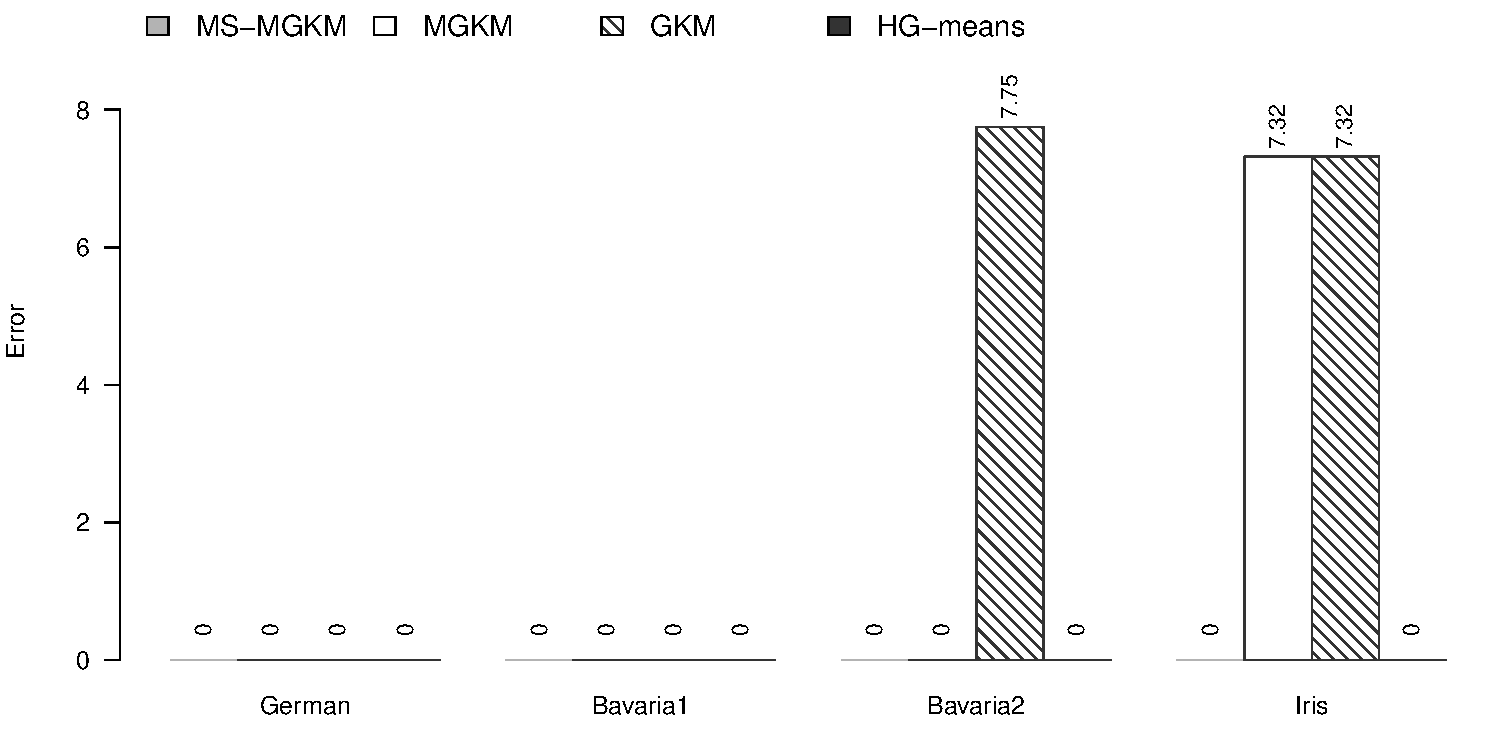
\includegraphics[width=1\textwidth]{img/error-A1-2}}
\subfigure[$m$ = 5]{\label{fig:error-A1-5}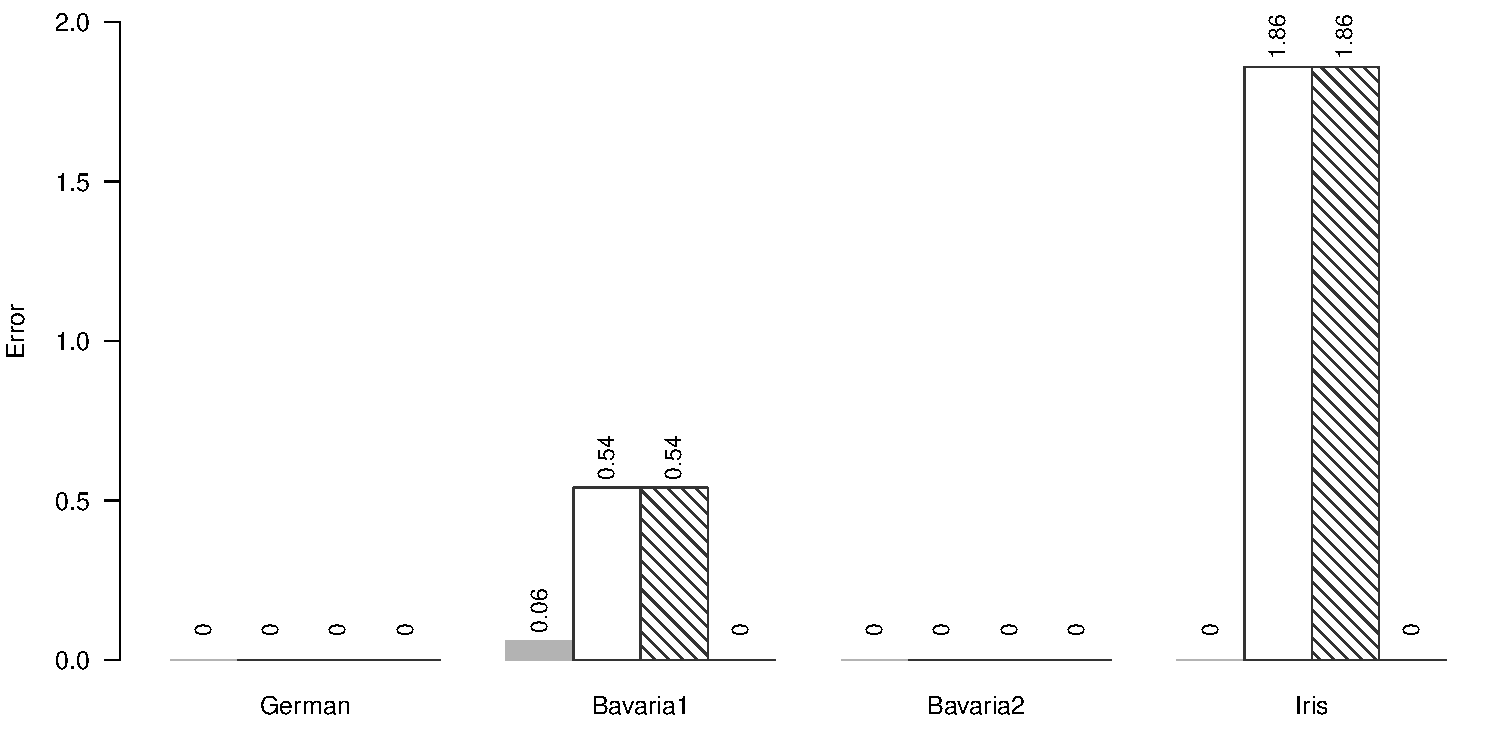
\includegraphics[width=1\textwidth]{img/error-A1-5}}
\subfigure[$m$ = 10]{\label{fig:error-A1-10}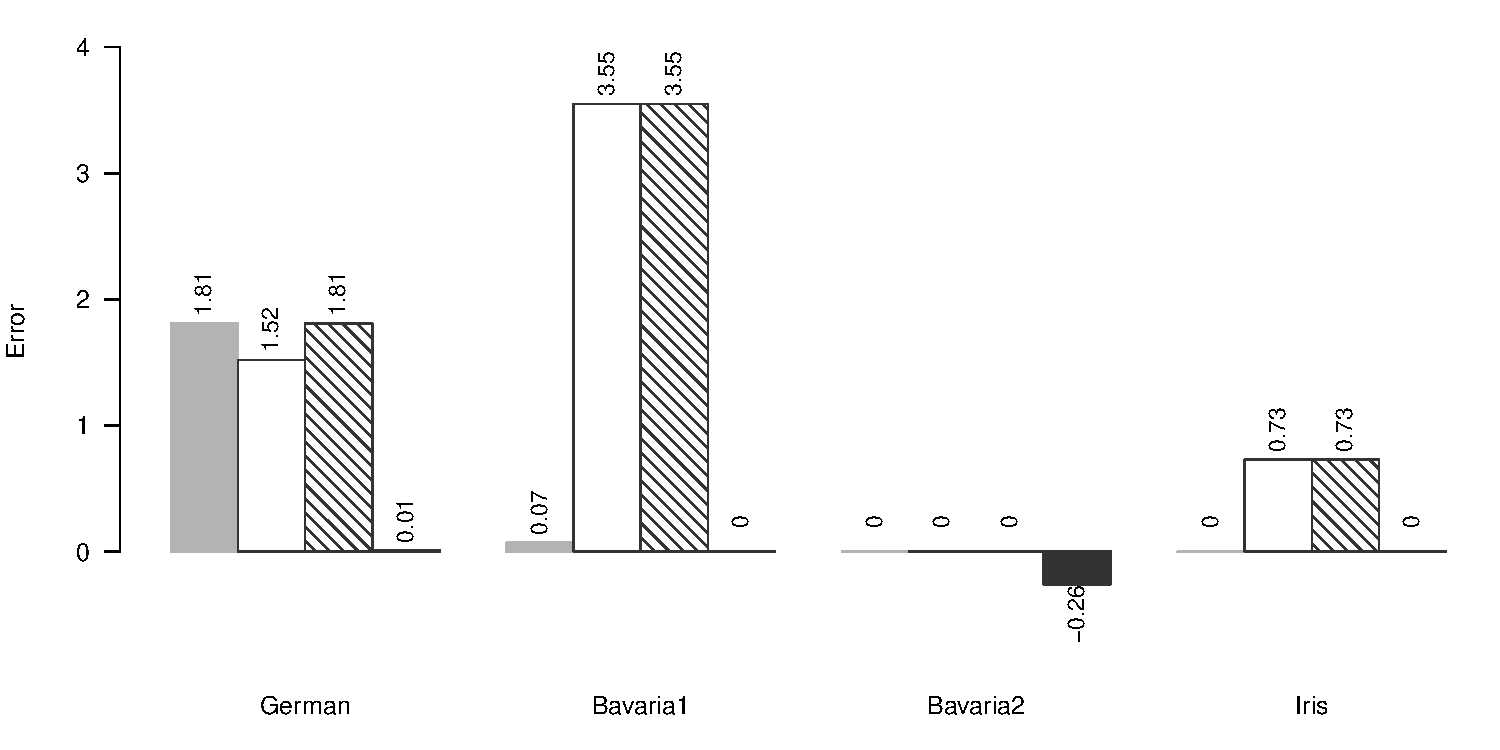
\includegraphics[width=1\textwidth]{img/error-A1-10}}
\caption{Algorithms performance for different number of clusters (Instances A1)}
\label{fig:error-A1}
\end{figure}

\begin{figure}[H]
\centering
\subfigure[$m$ = 10]{\label{fig:error-A2-10}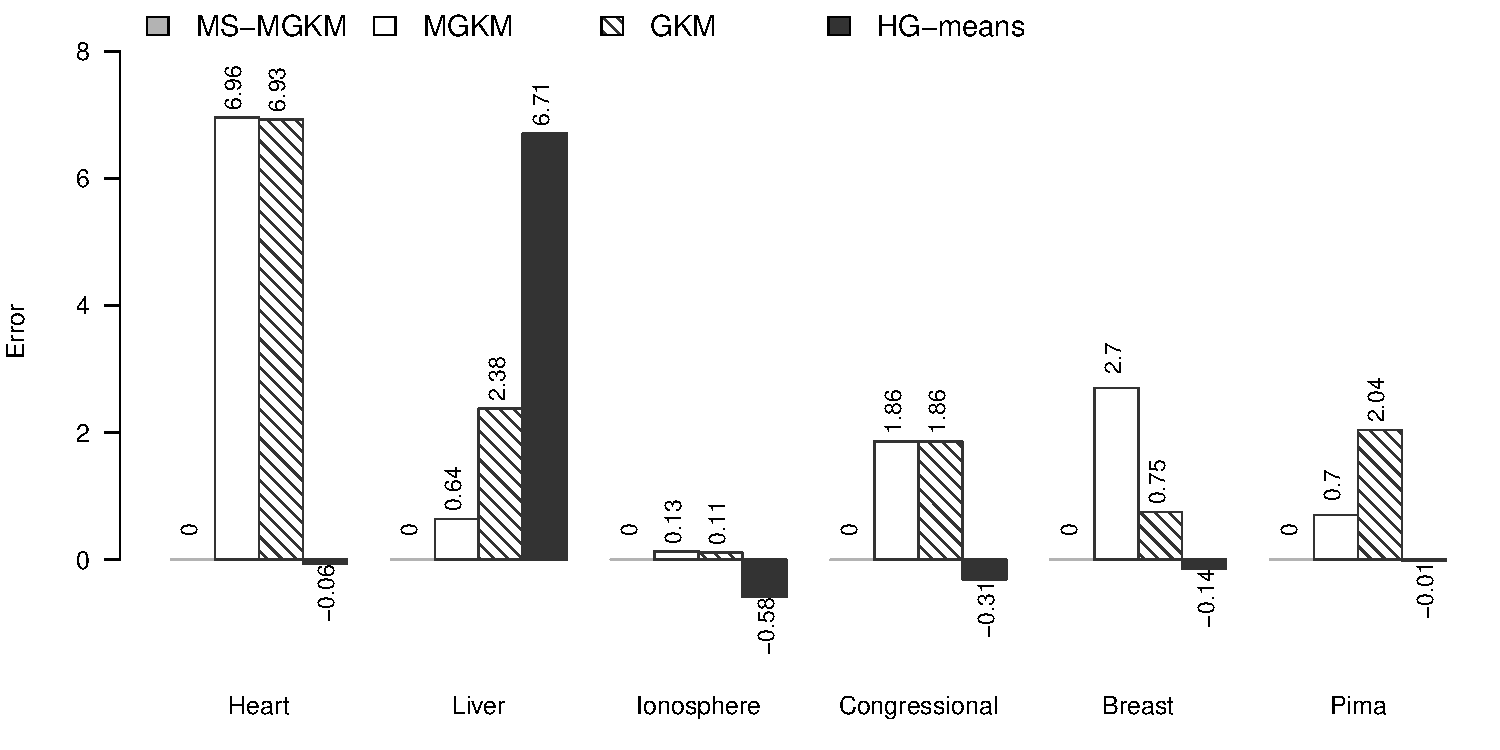
\includegraphics[width=1\textwidth]{img/error-A2-10}}
\subfigure[$m$ = 30]{\label{fig:error-A2-30}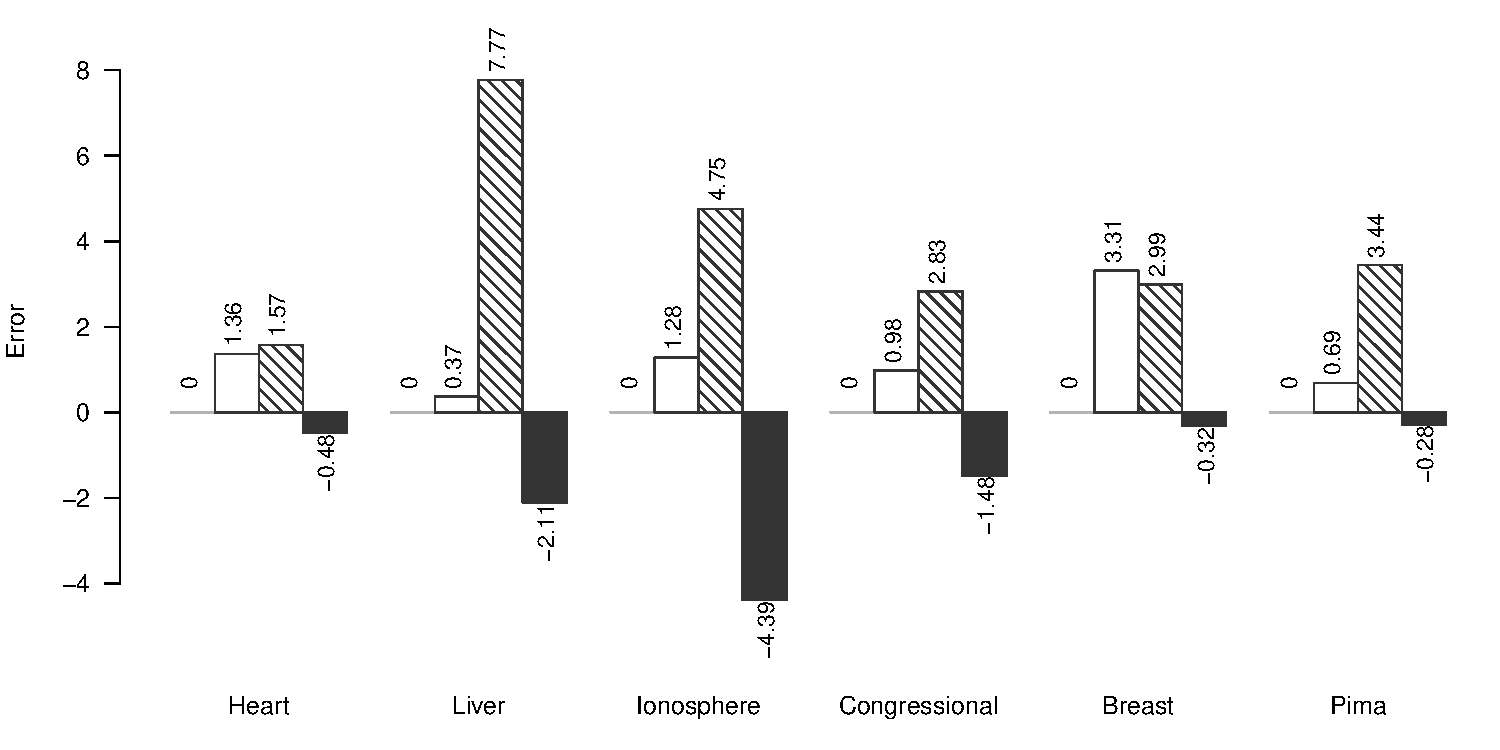
\includegraphics[width=1\textwidth]{img/error-A2-30}}
\subfigure[$m$ = 50]{\label{fig:error-A2-50}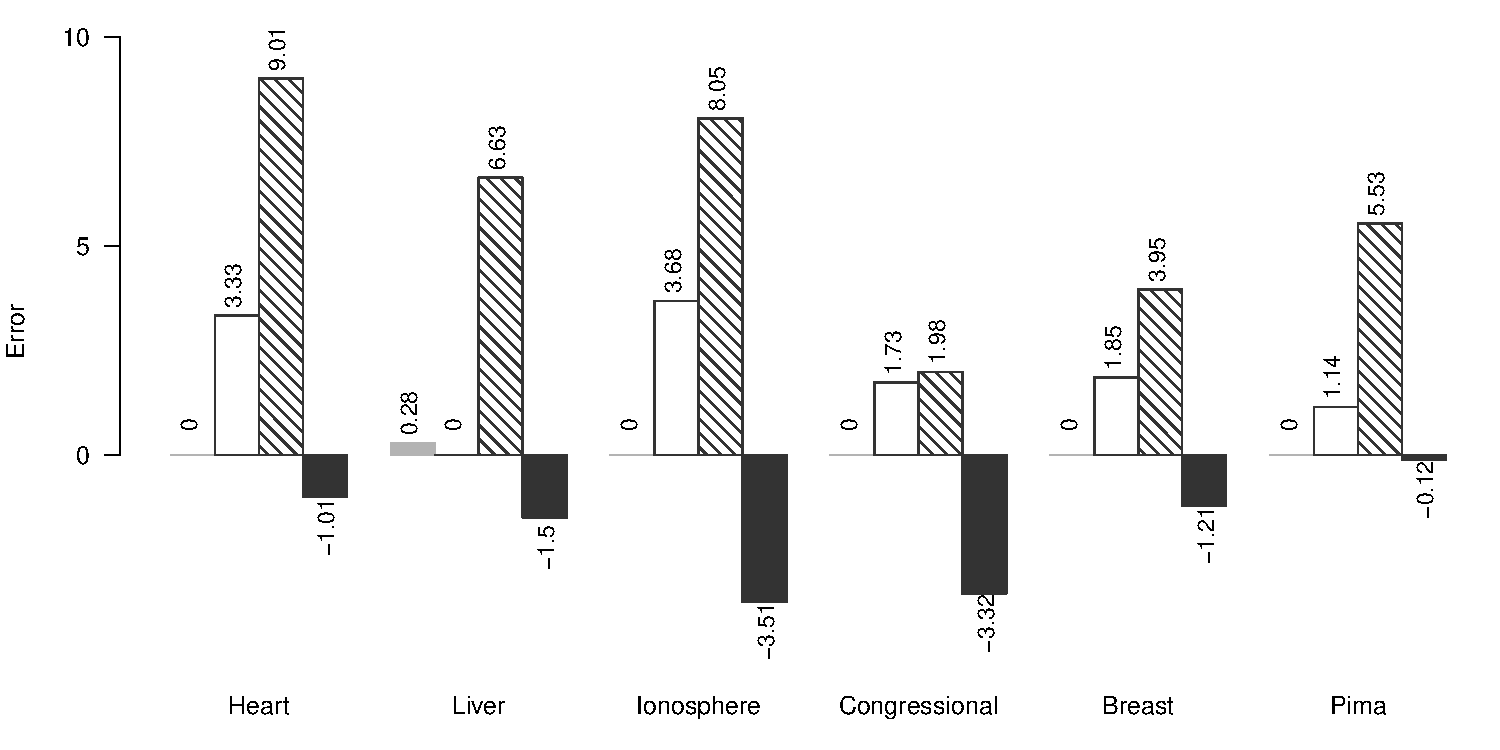
\includegraphics[width=1\textwidth]{img/error-A2-50}}
\caption{Algorithms performance for different number of clusters (Instances A2)}
\label{fig:error-A2}
\end{figure}

\begin{figure}[H]
\centering
\subfigure[$m$ = 20]{\label{fig:error-B-20}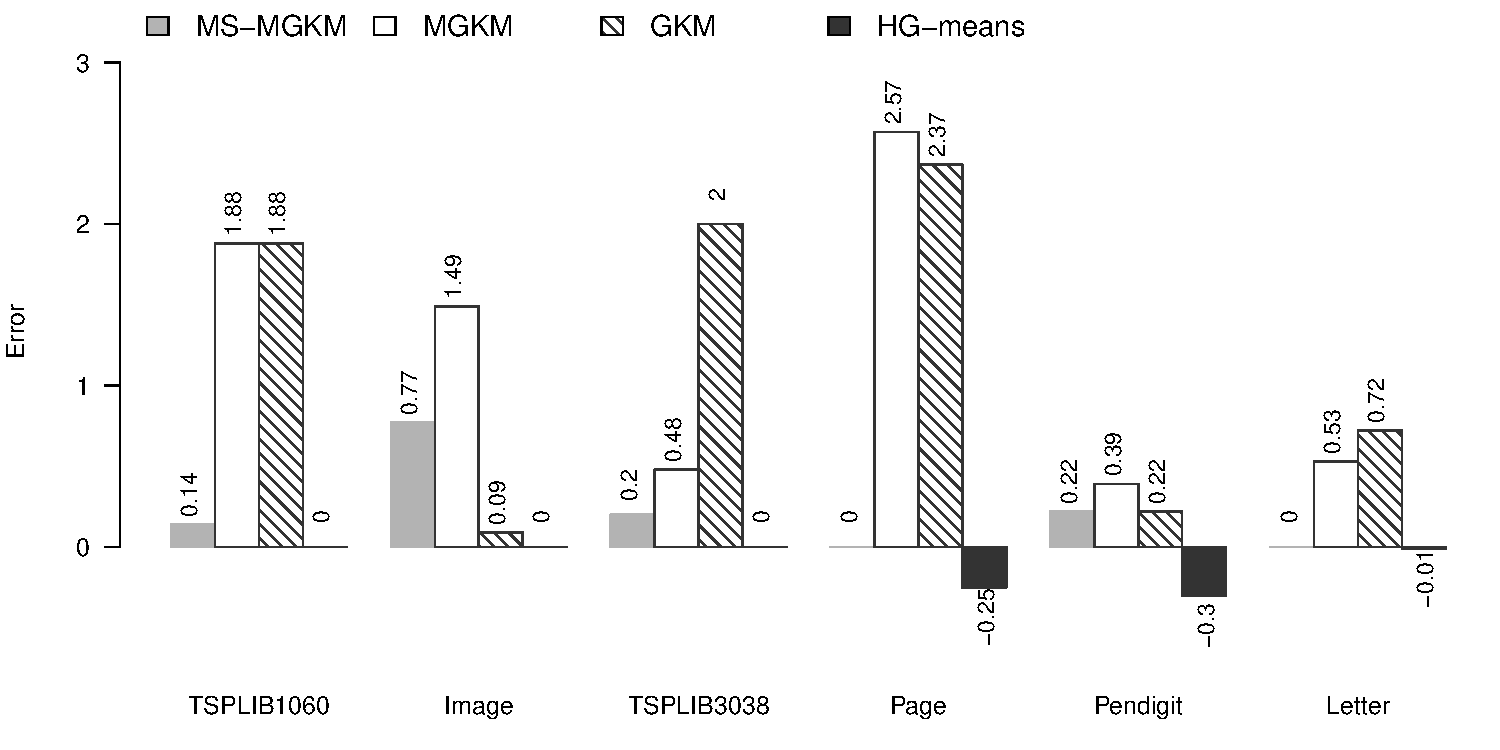
\includegraphics[width=1\textwidth]{img/error-B-20}}
\subfigure[$m$ = 40]{\label{fig:error-B-40}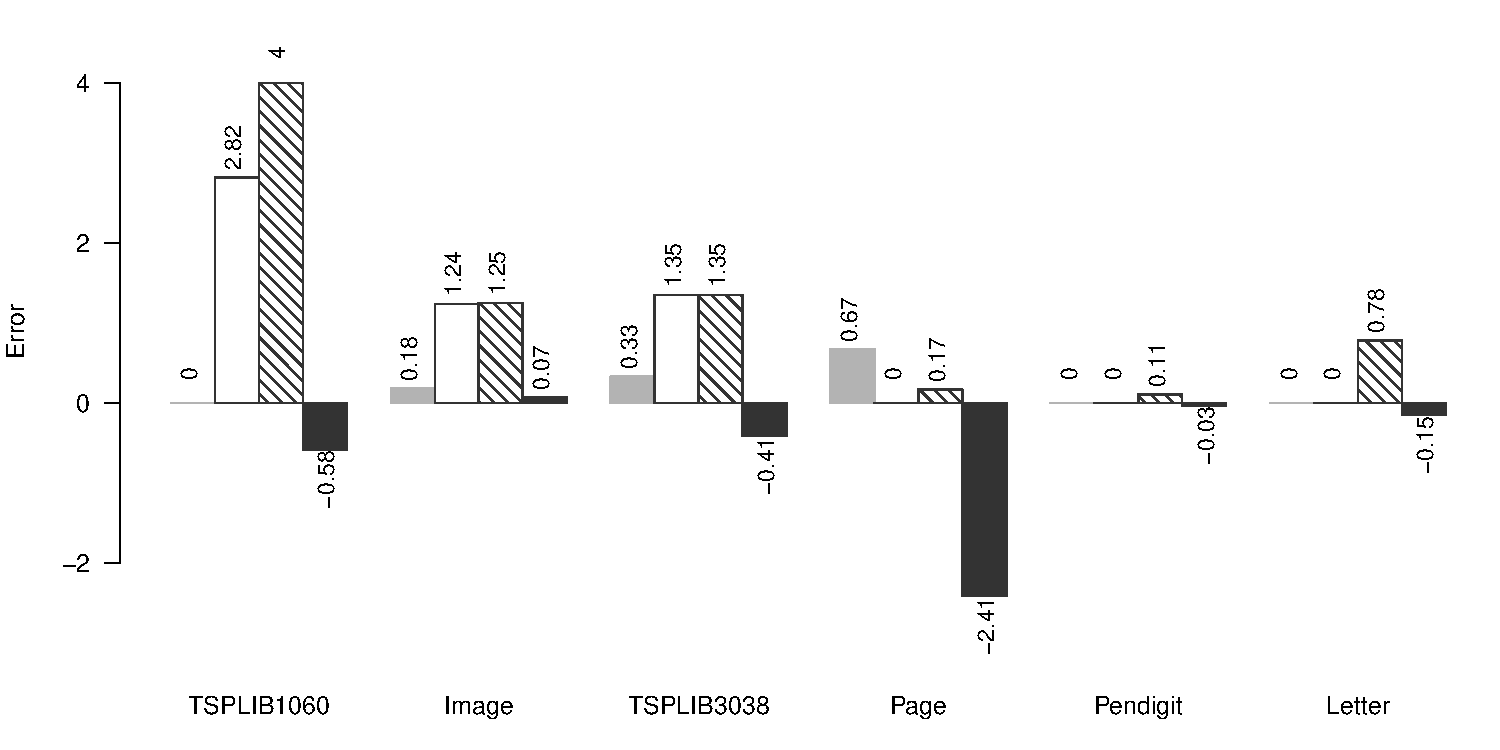
\includegraphics[width=1\textwidth]{img/error-B-40}}
\subfigure[$m$ = 80]{\label{fig:error-B-80}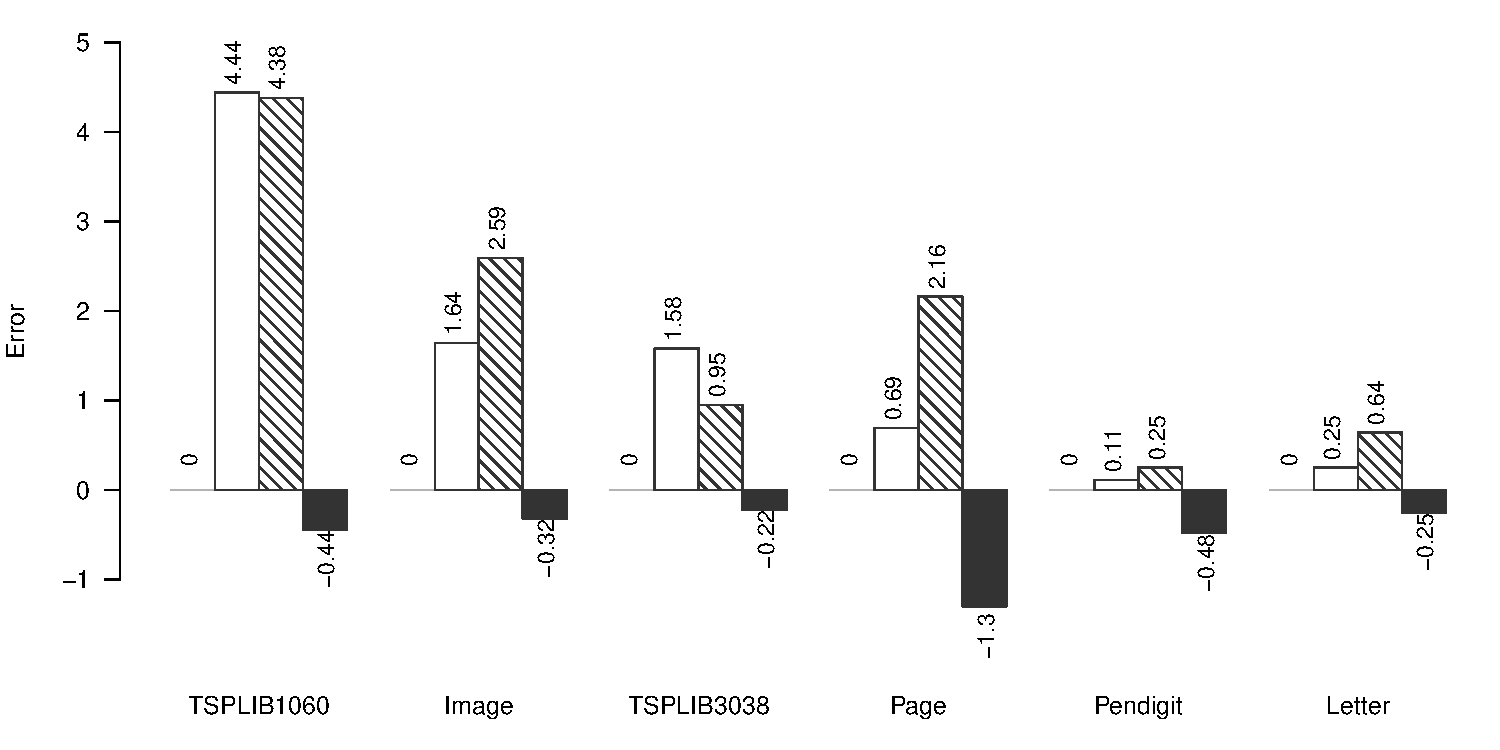
\includegraphics[width=1\textwidth]{img/error-B-80}}
\caption{Algorithms performance for different number of clusters (Instances B)}
\label{fig:error-B}
\end{figure}

\begin{figure}[H]
\centering
\subfigure[$m$ = 15]{\label{fig:error-C-15}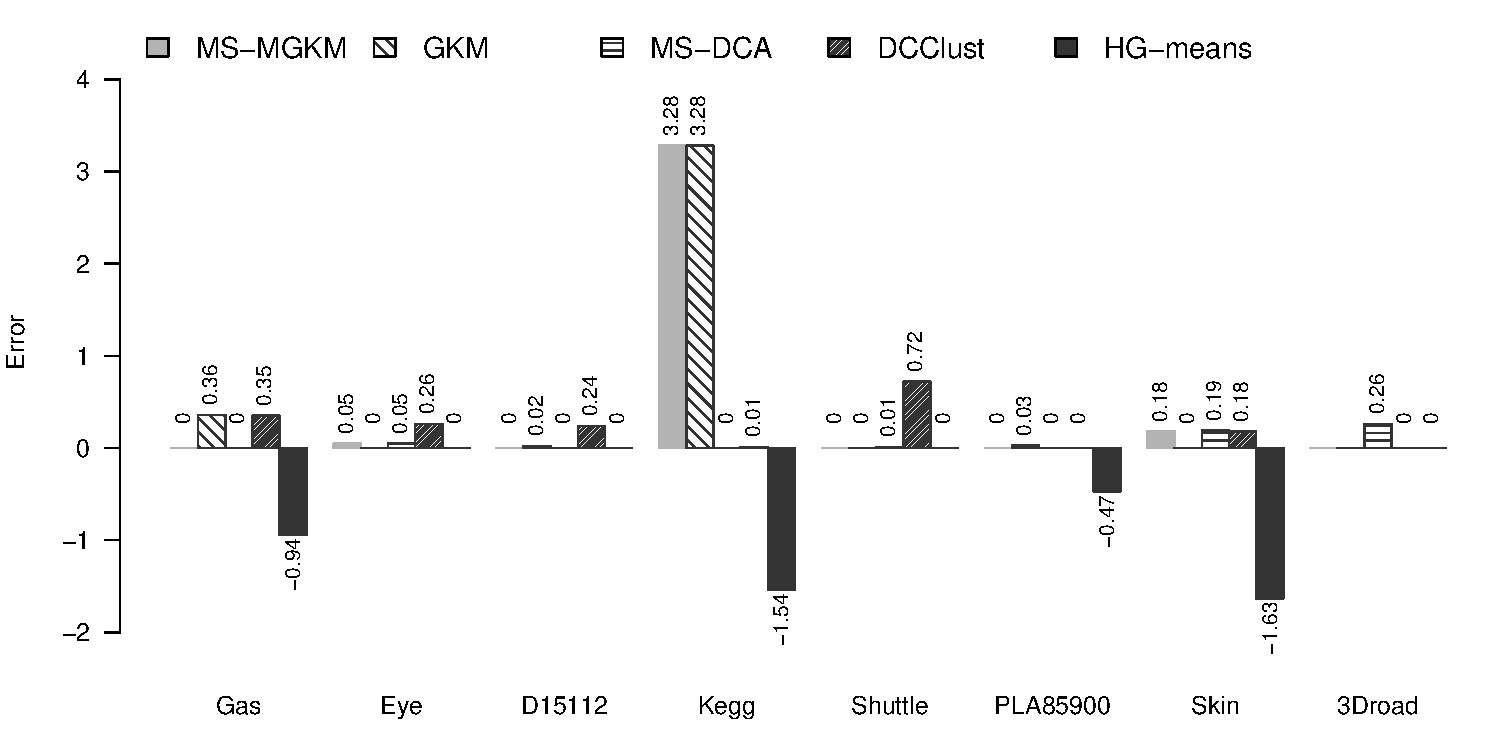
\includegraphics[width=1\textwidth]{img/error-C-15}}
\subfigure[$m$ = 20]{\label{fig:error-C-20}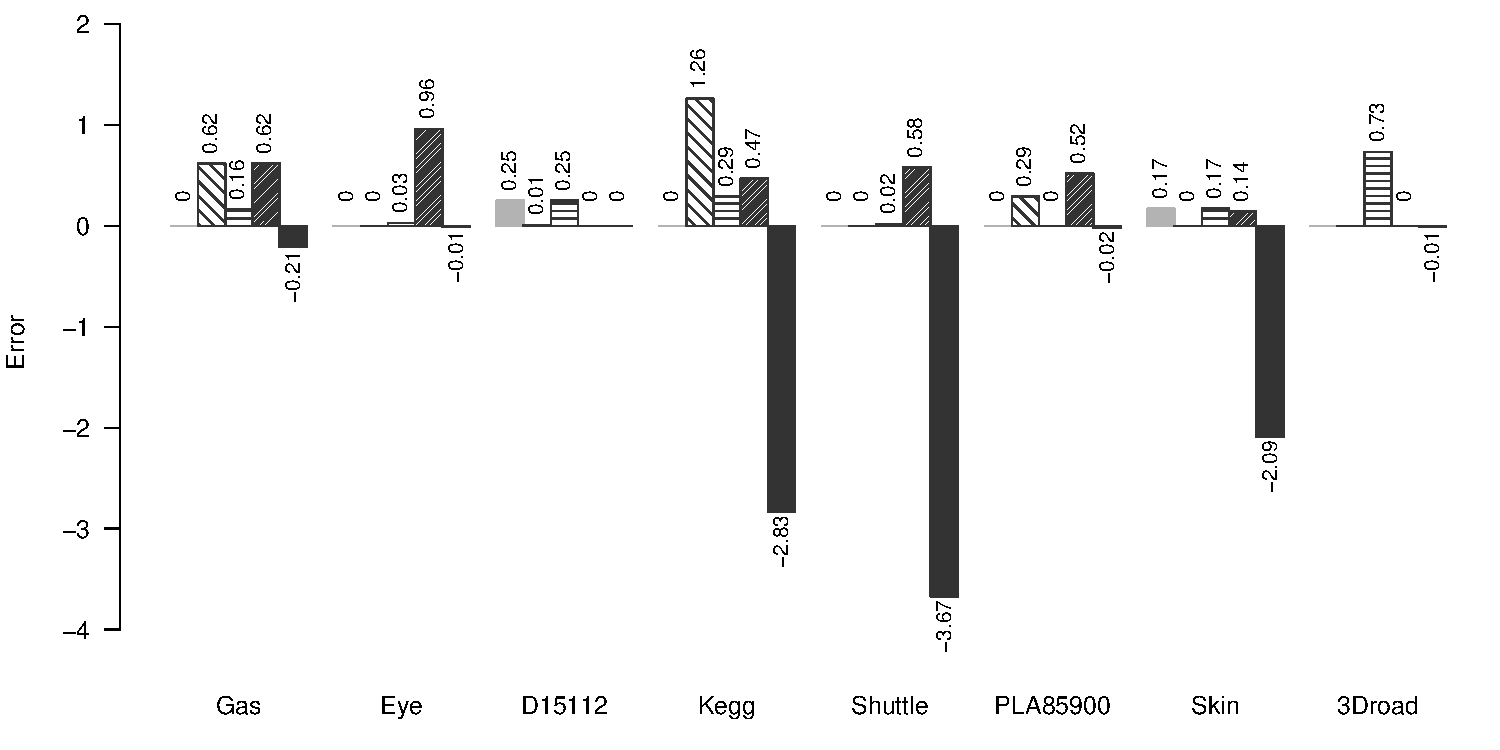
\includegraphics[width=1\textwidth]{img/error-C-20}}
\subfigure[$m$ = 25]{\label{fig:error-C-25}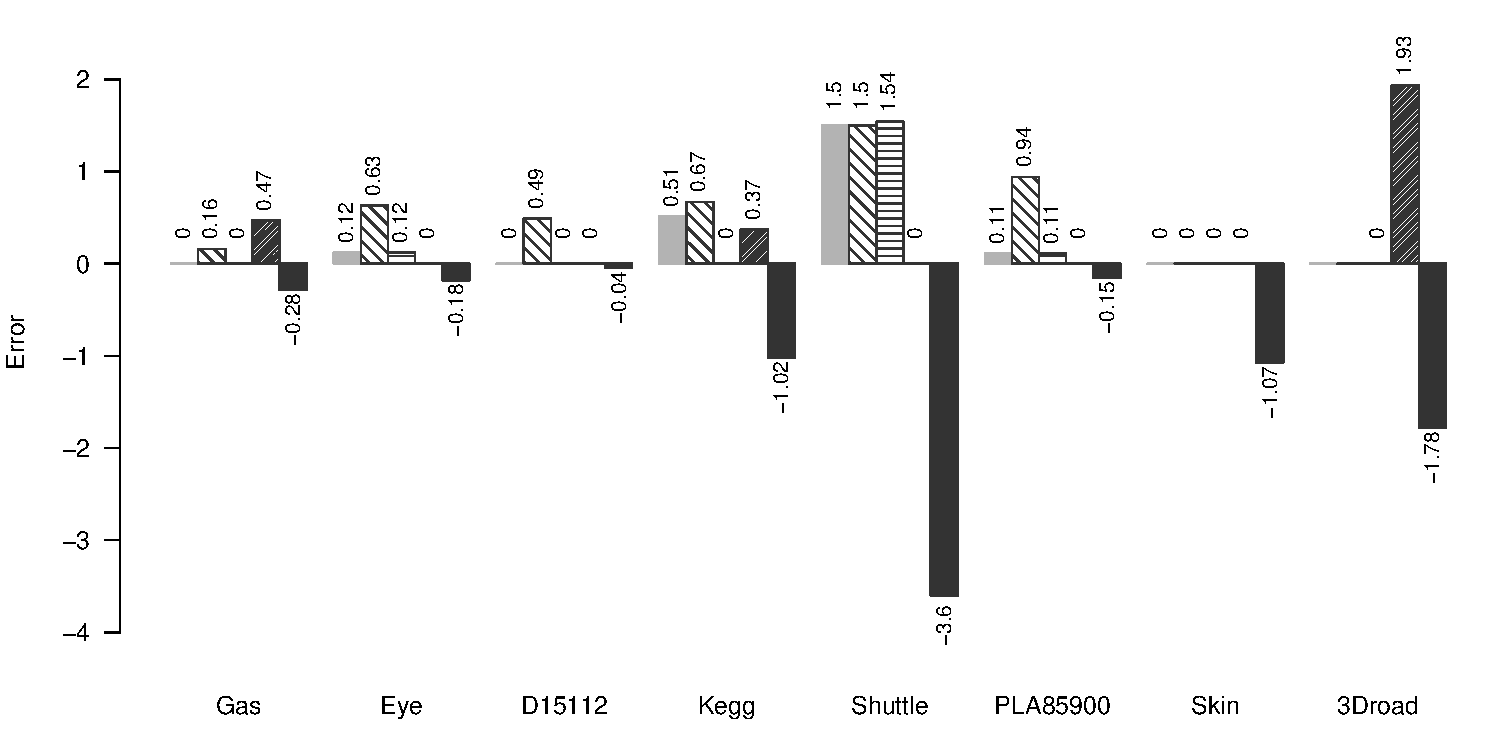
\includegraphics[width=1\textwidth]{img/error-C-25}}
\caption{Algorithms performance for different number of clusters (Instances C)}
\label{fig:error-C}
\end{figure}

\subsection{Impact of instances size}
Section \ref{sec:performance} shows that the objective value of solutions produced by HG-means outperformed the compared algorithms in most experiments. This section presents some analysis regarding the HG-means scaling, i.e., how much computational time does the algorithm require in large data. Figures \ref{fig:timeB} and \ref{fig:timeC} compare HG-means with MS-MGKM, MGKM, GKM and DCClust in terms of CPU time as a function of the number of clusters $m$. The elapsed time was measured in seconds and the results are presented for groups B and C of instances. For small instances, there is a very small difference in the computational time of the considered algorithms. Therefore, the results for groups A1 and A2 are not presented in this analysis.

%For instances of group A2, HG-means demands more computational efforts than MS-MGKM, MGKM, GKM and DCClust for all values of $m$.
For group B of instances, HG-means takes a similar amount of time when compared to other algorithms, and has its most competitive performance when $m$ is increased. For instances of group C, HG-means is faster than the other algorithms exactly in the largest instances (Pla85900, Skin segmentation and 3D road), having a similar computational time for the remaining instances in this group.

Therefore, HG-means is very promising regarding scalability, as it produces better solutions and requires less computational time than the compared algorithms on large instances. In addition, there is room to adjust the number of iterations the algorithm takes and to use more efficient data structures that can improve runtime.

%\begin{figure}[H]
%\centering
%\subfigure[$m$ = 2]{\label{fig:sizeB-2}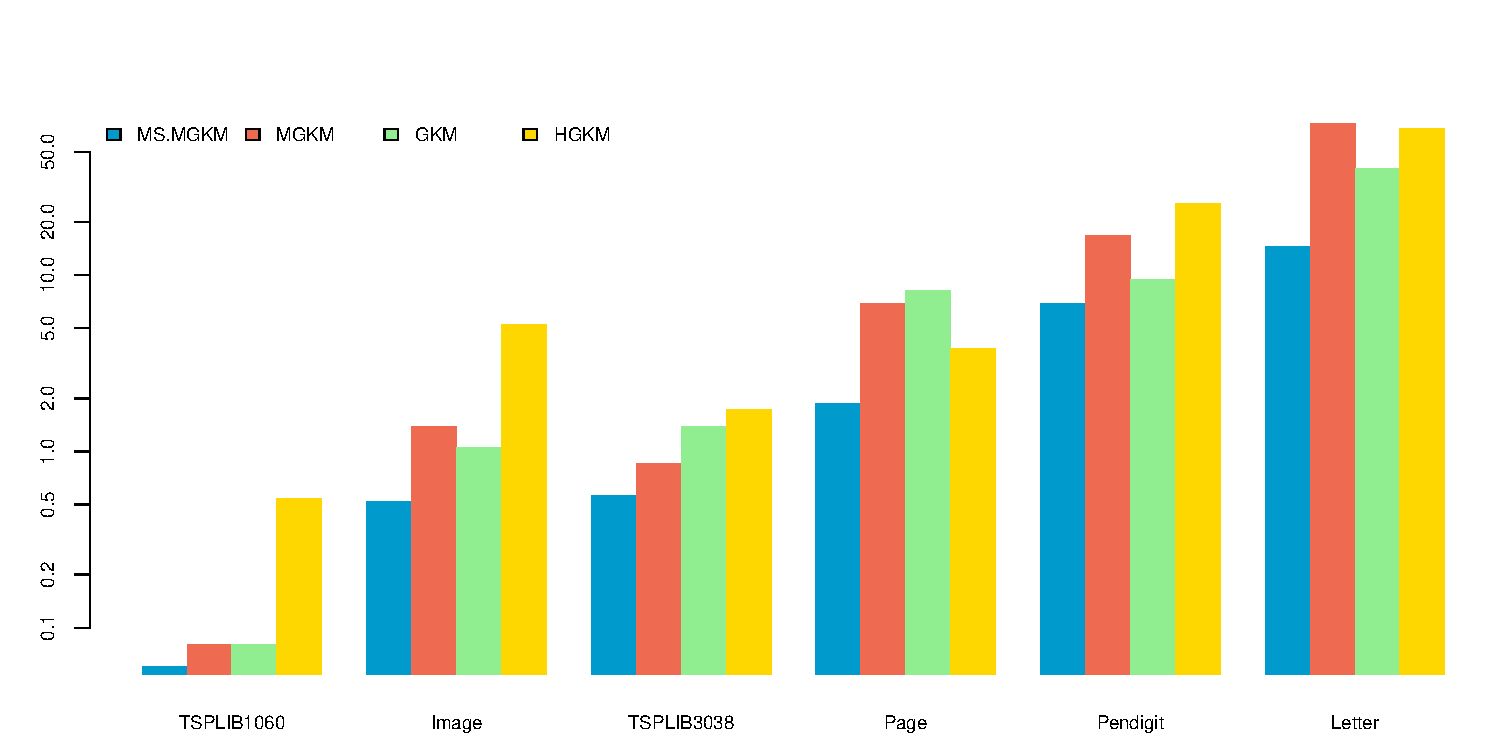
\includegraphics[width=1\textwidth]{img/sizeB-2}}
%\subfigure[$m$ = 10]{\label{fig:sizeB-10}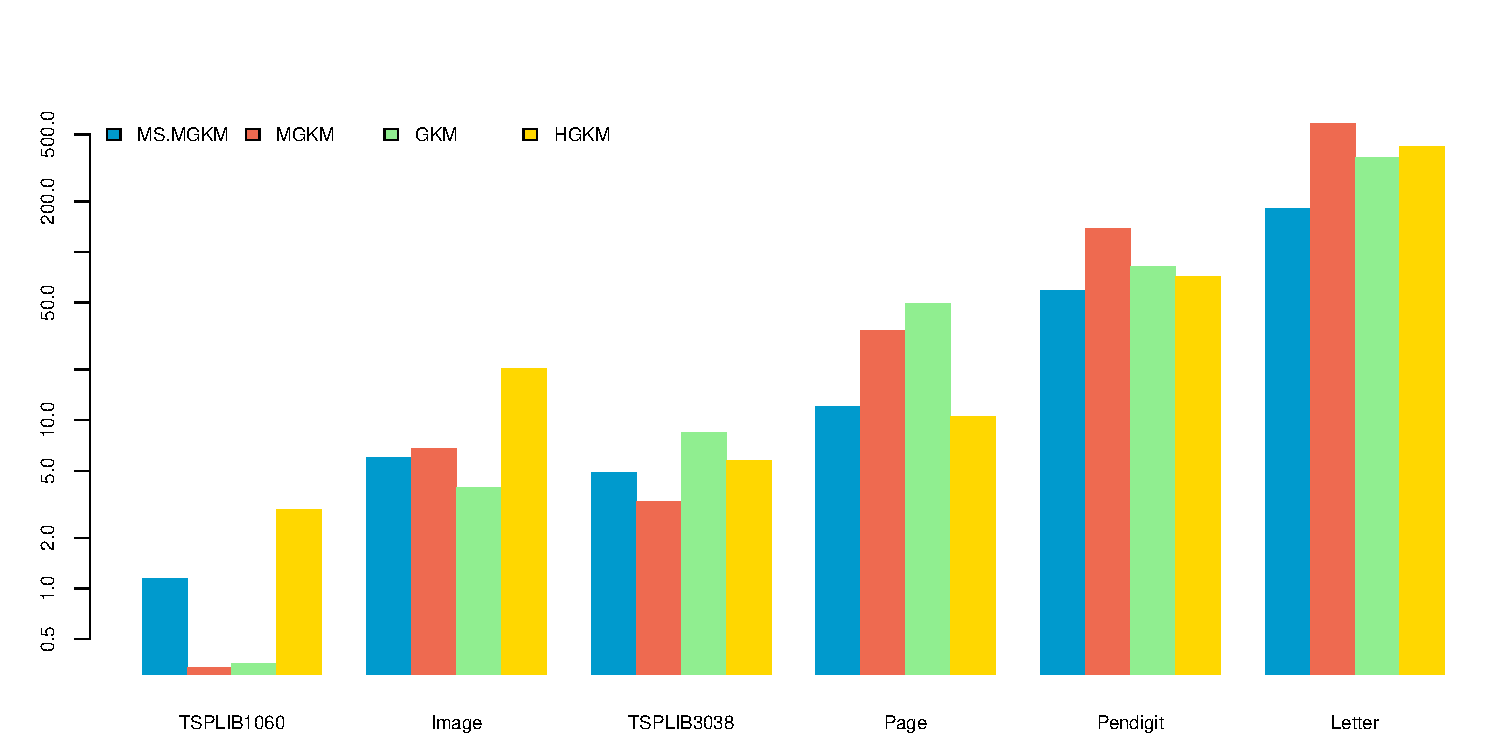
\includegraphics[width=1\textwidth]{img/sizeB-10}}
%\subfigure[$m$ = 20]{\label{fig:sizeB-20}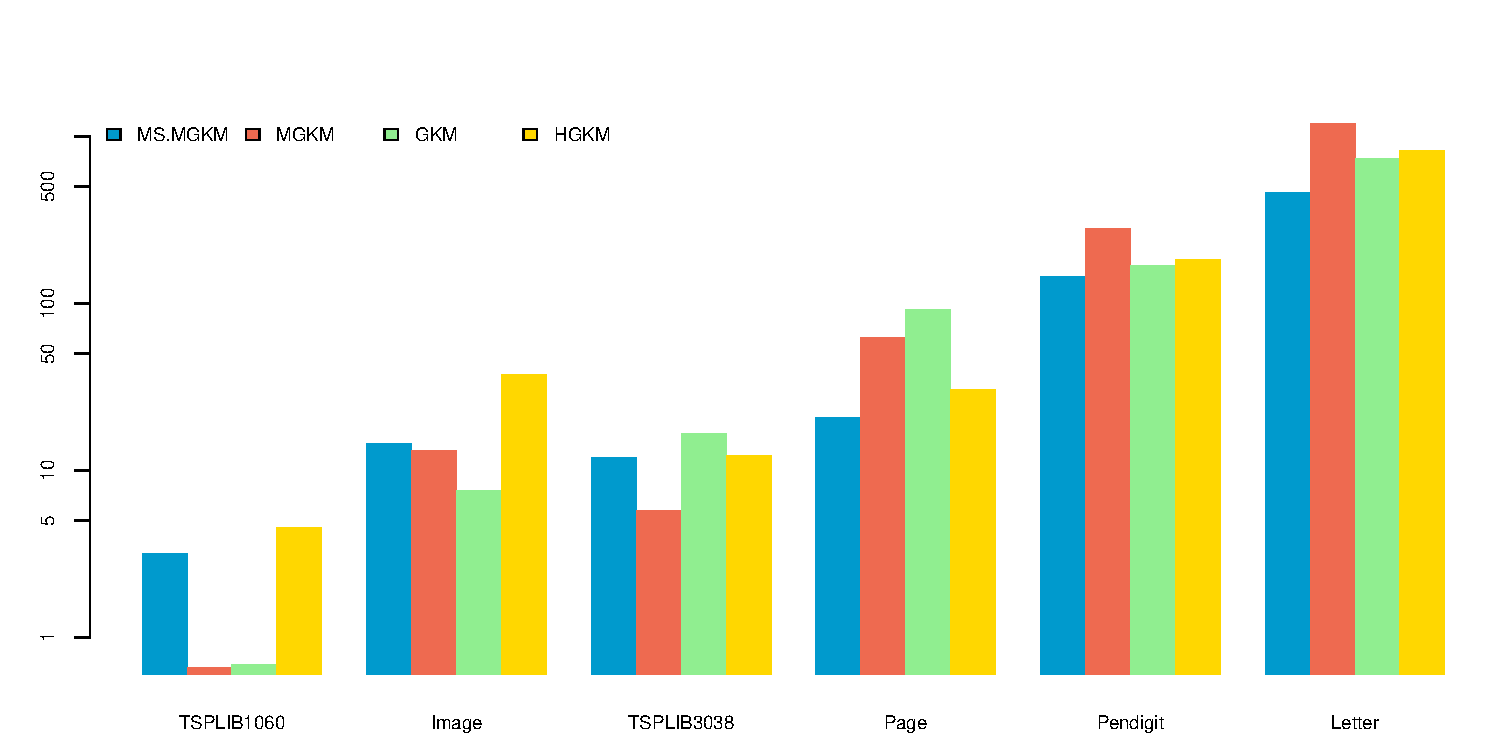
\includegraphics[width=1\textwidth]{img/sizeB-20}}
%\caption{The CPU time of algorithms in instances of group B}
%\label{fig:sizeB}
%\end{figure}
%
%\begin{figure}[H]
%\centering
%\subfigure[$m$ = 2]{\label{fig:sizeC-2}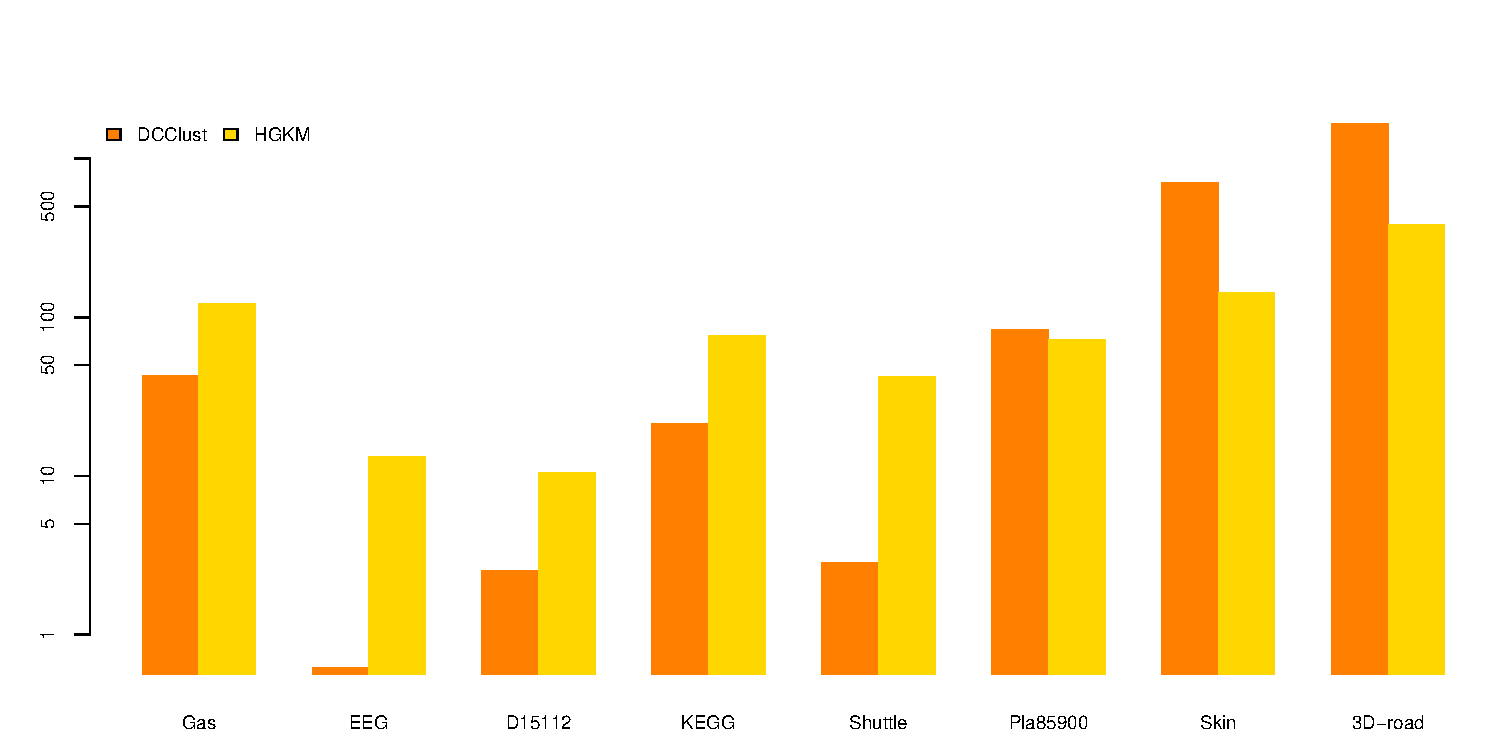
\includegraphics[width=1\textwidth]{img/sizeC-2}}
%\subfigure[$m$ = 10]{\label{fig:sizeC-10}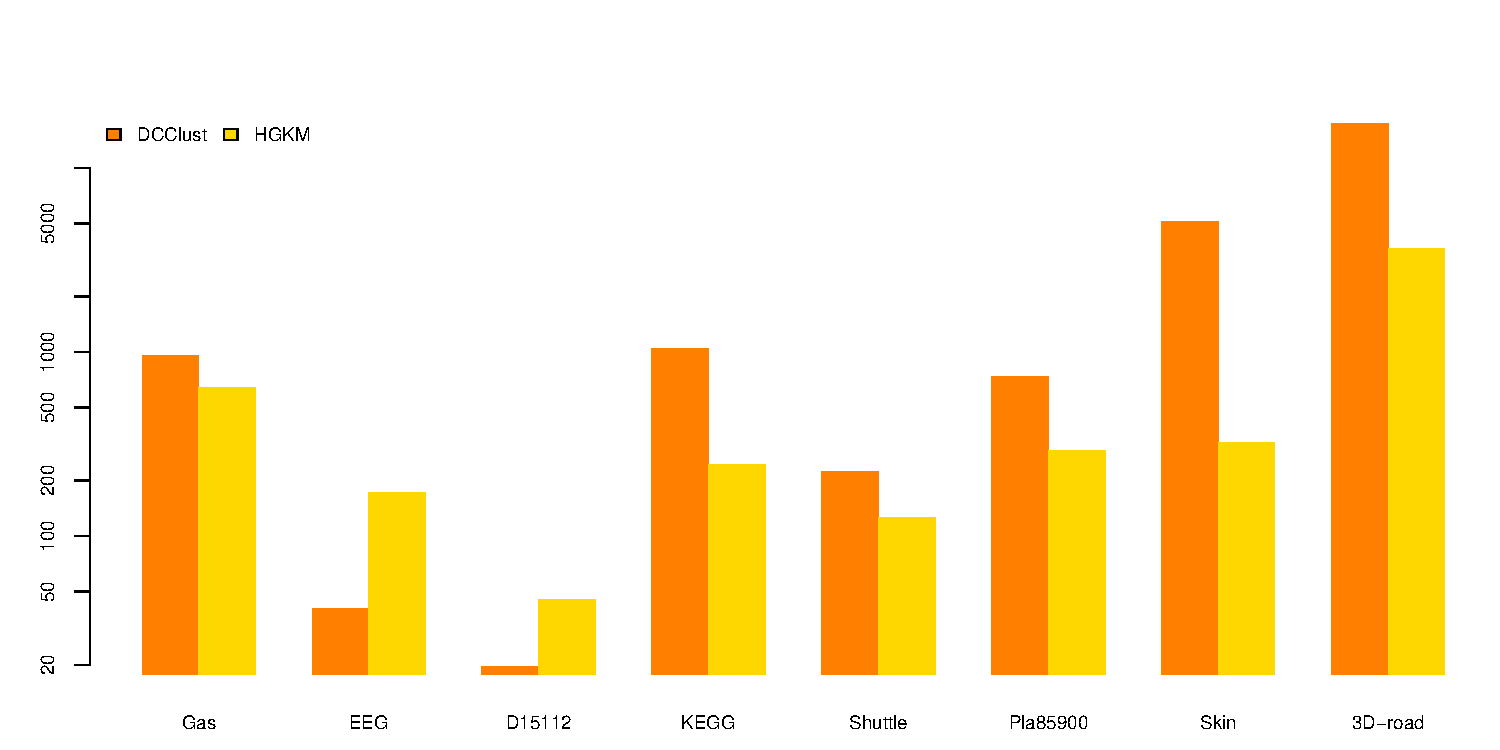
\includegraphics[width=1\textwidth]{img/sizeC-10}}
%\subfigure[$m$ = 20]{\label{fig:sizeC-20}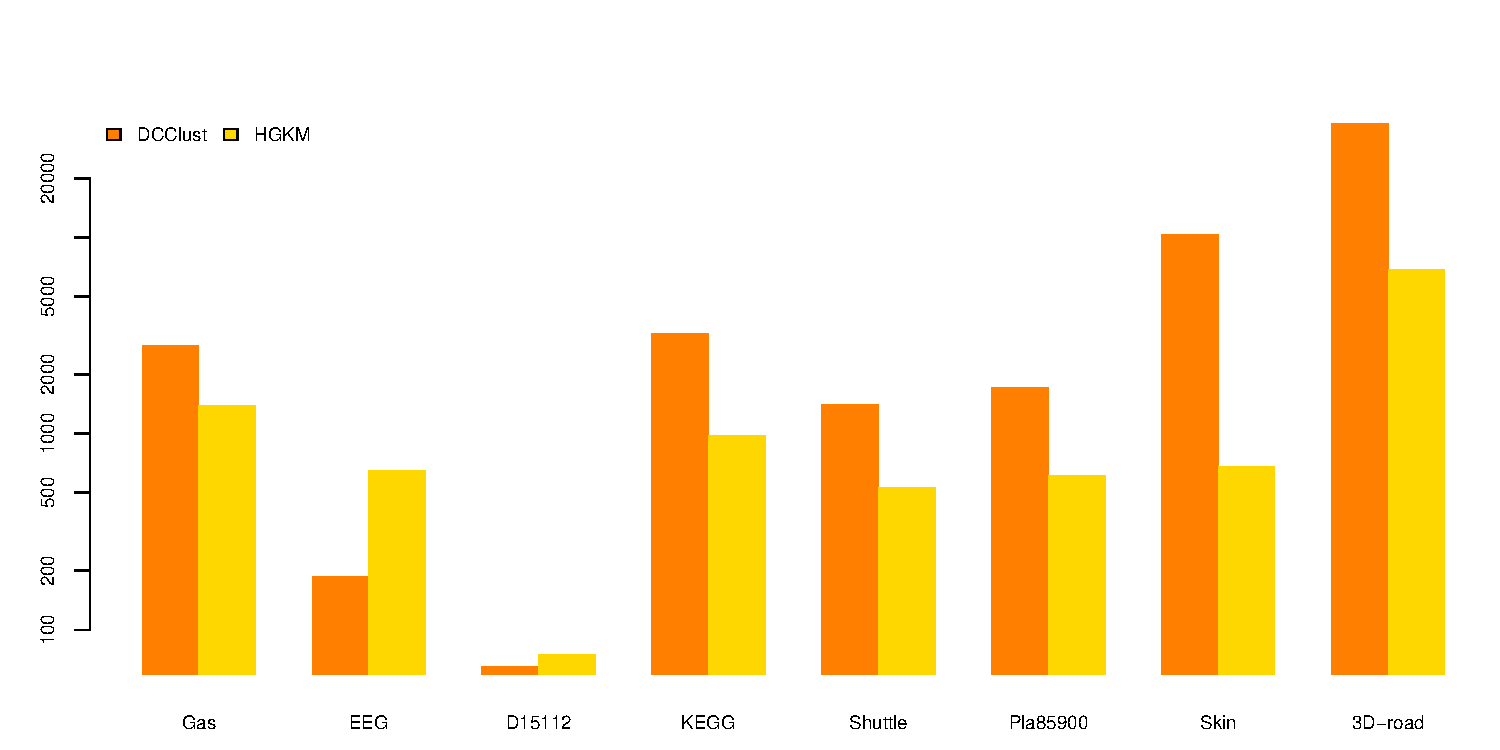
\includegraphics[width=1\textwidth]{img/sizeC-20}}
%\caption{The CPU time of algorithms in instances of group C}
%\label{fig:sizeC}
%\end{figure}

%%%%%%%%%%%%%%%%%%%%%

\begin{figure}[H]
\centering
\subfigure[TSPLIB1060 ($n$ = 1060)]{\label{fig:time1}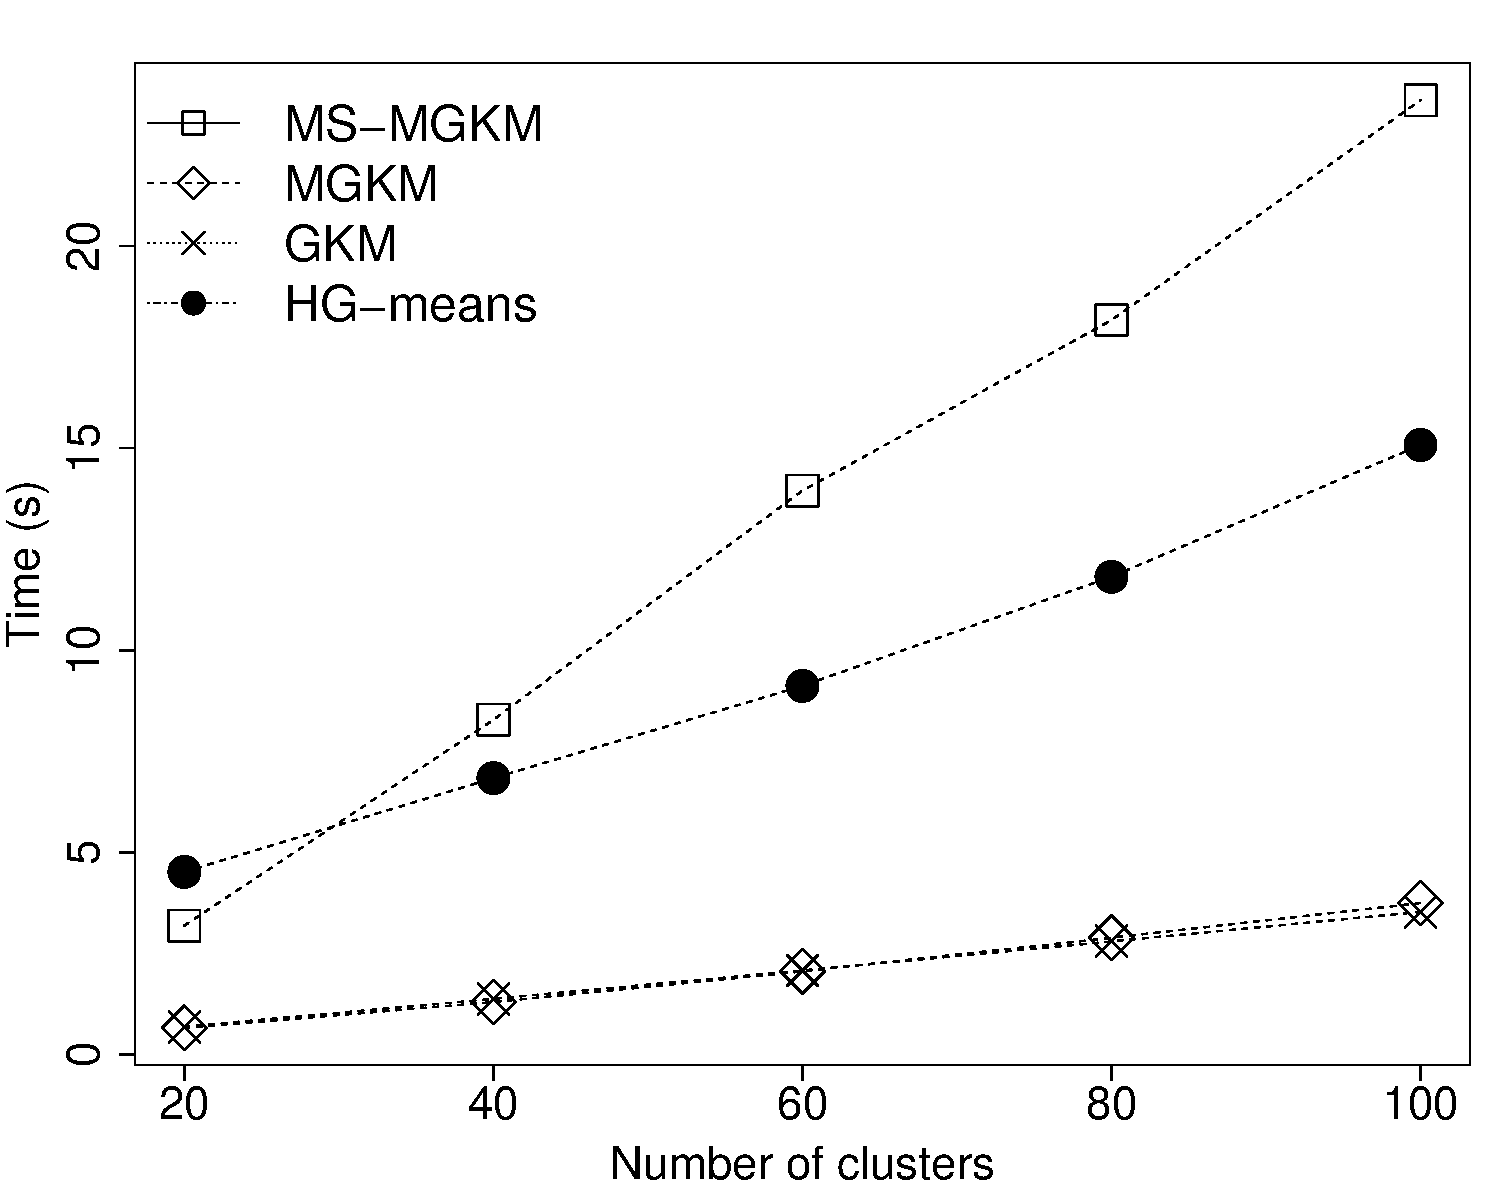
\includegraphics[width=0.48\textwidth]{img/cpu-tsplib1060}}
\subfigure[Image segmentation ($n$ = 2310)]{\label{fig:time2}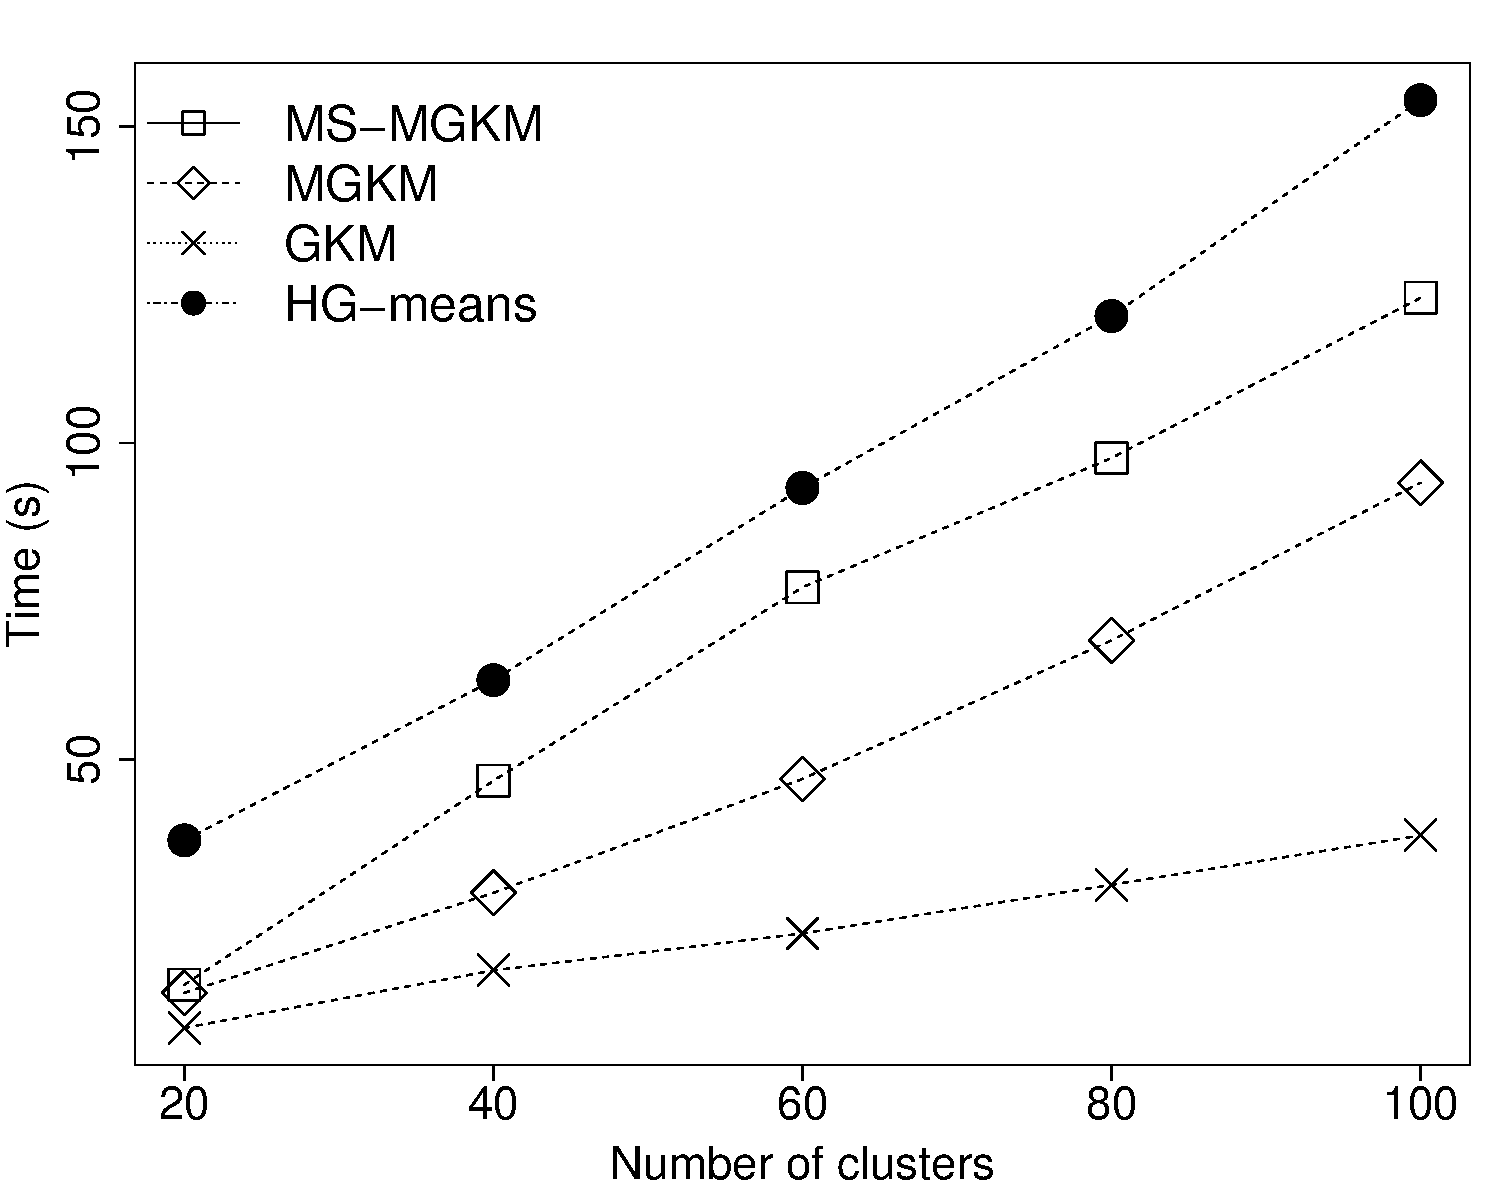
\includegraphics[width=0.48\textwidth]{img/cpu-image}}
\subfigure[TSPLIB3038 ($n$ = 3038)]{\label{fig:time3}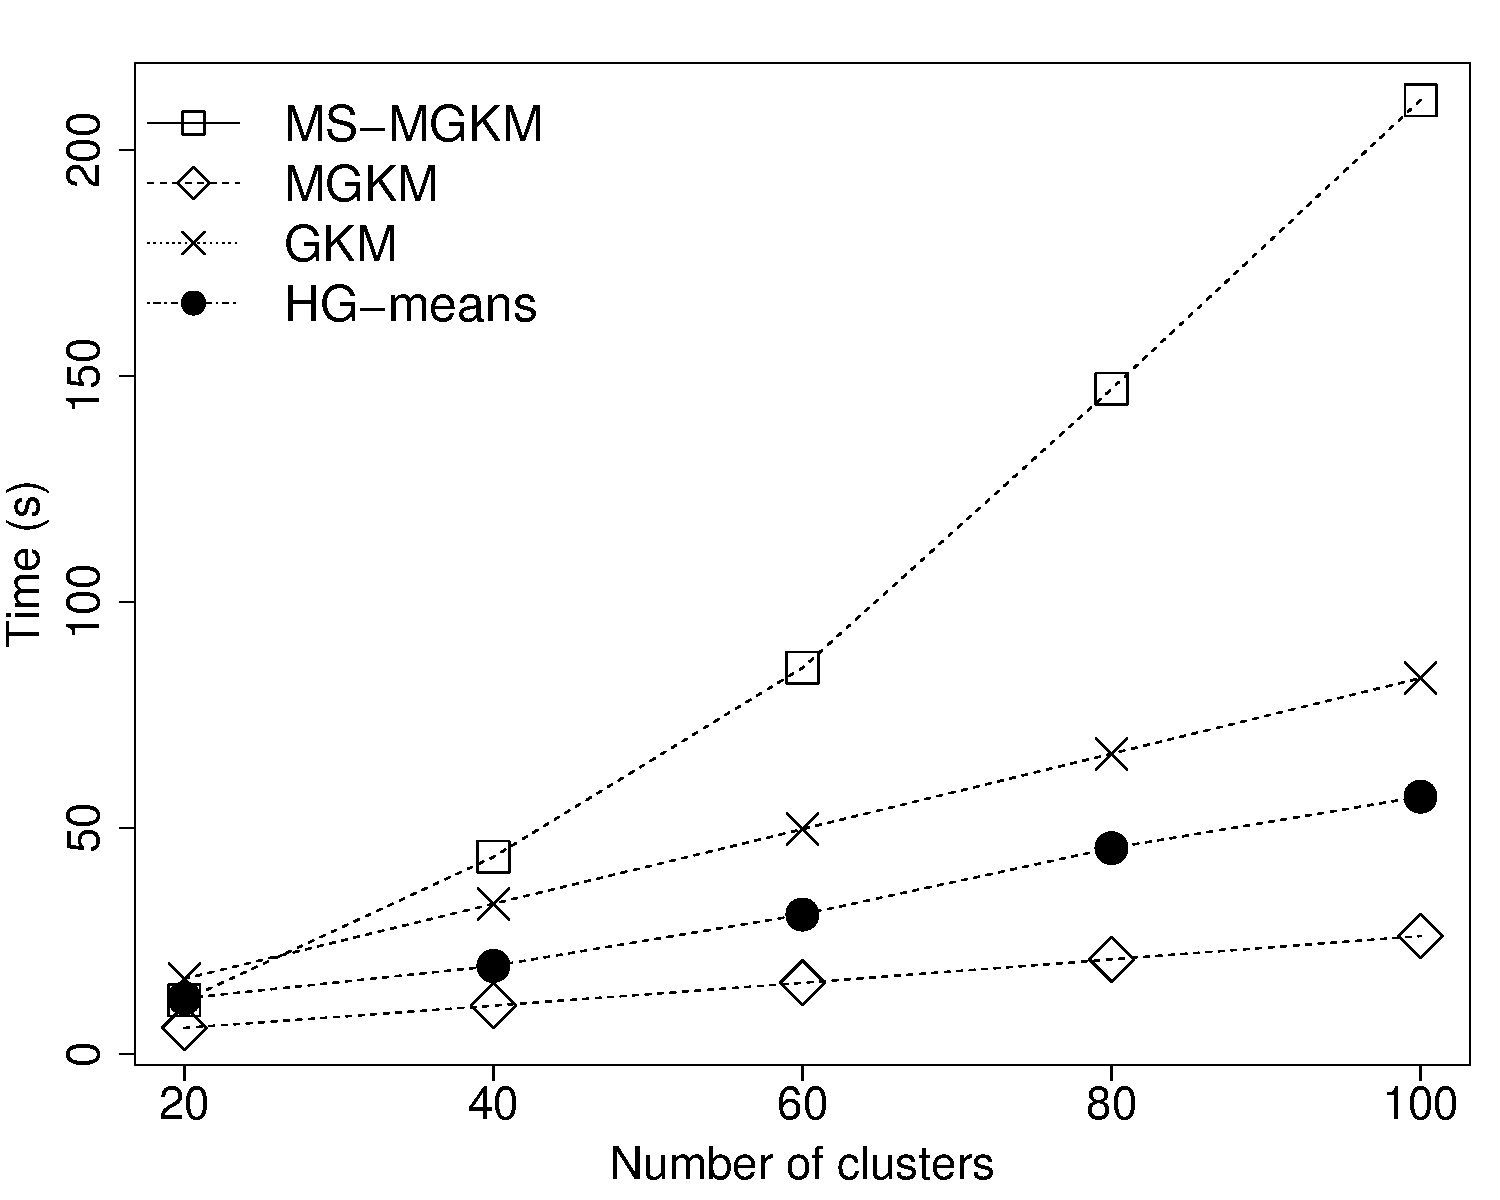
\includegraphics[width=0.48\textwidth]{img/cpu-tsplib3038}}
\subfigure[Page blocks ($n$ = 5473)]{\label{fig:time4}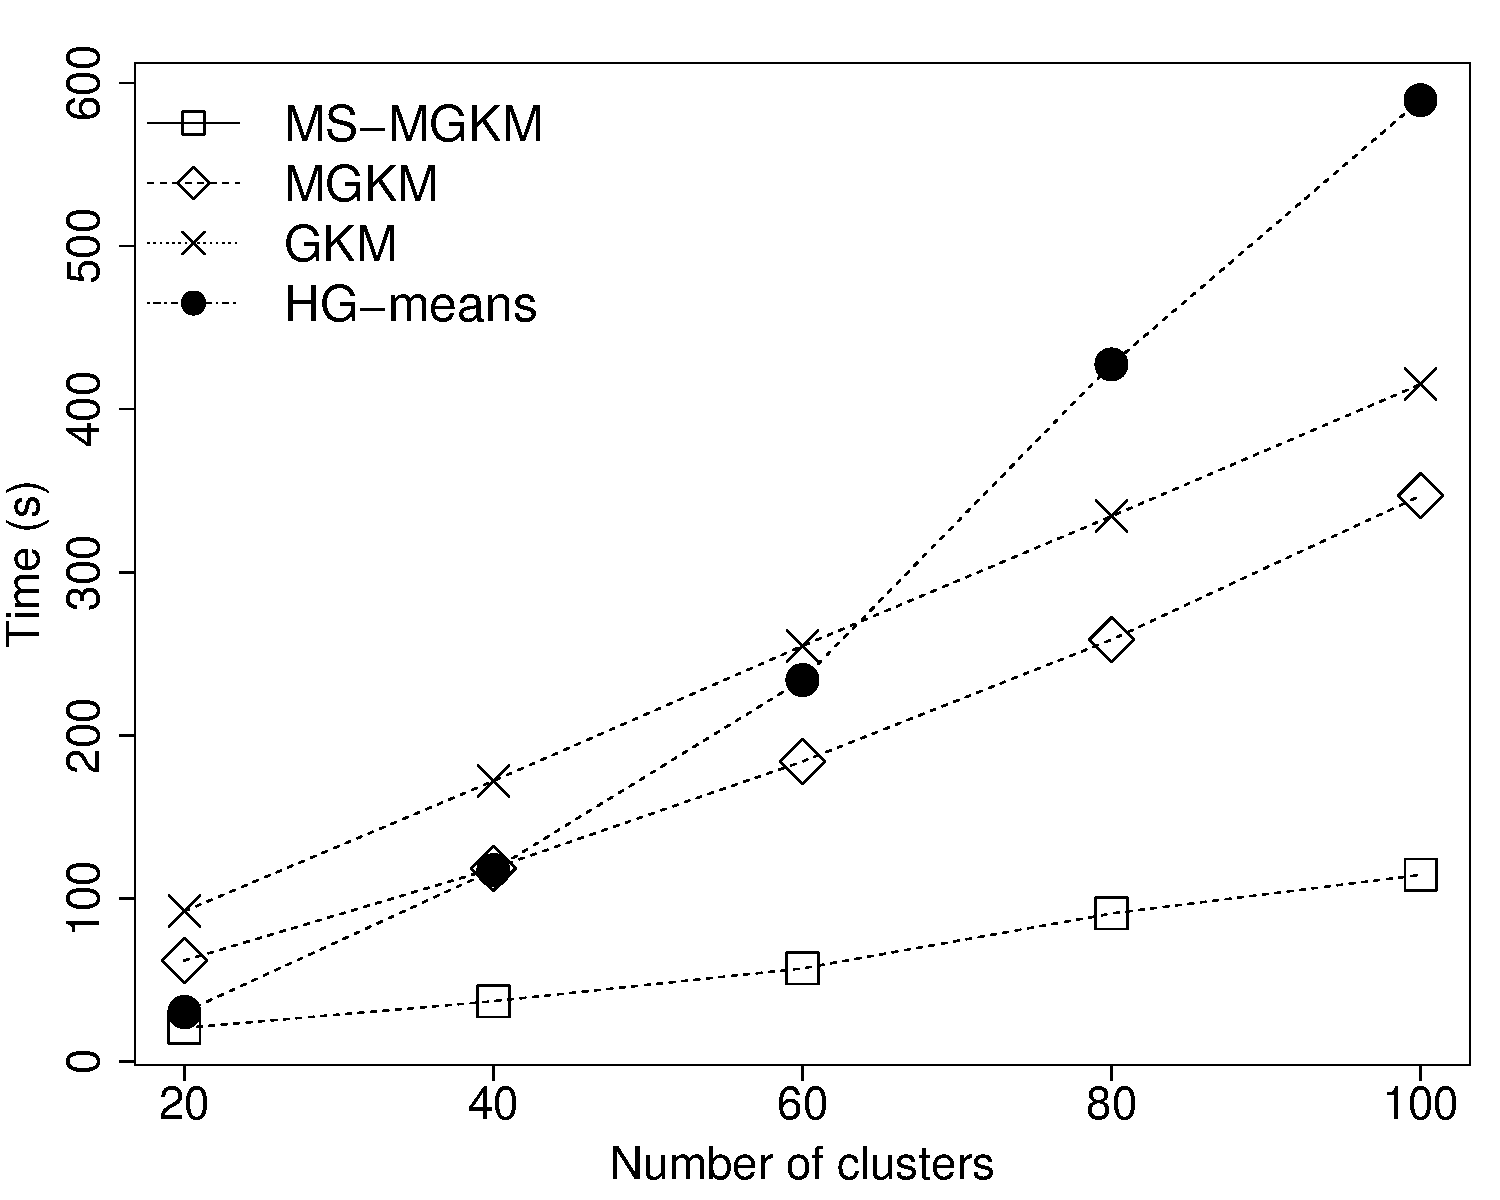
\includegraphics[width=0.48\textwidth]{img/cpu-page}}
\subfigure[Pendigit ($n$ = 10992)]{\label{fig:time5}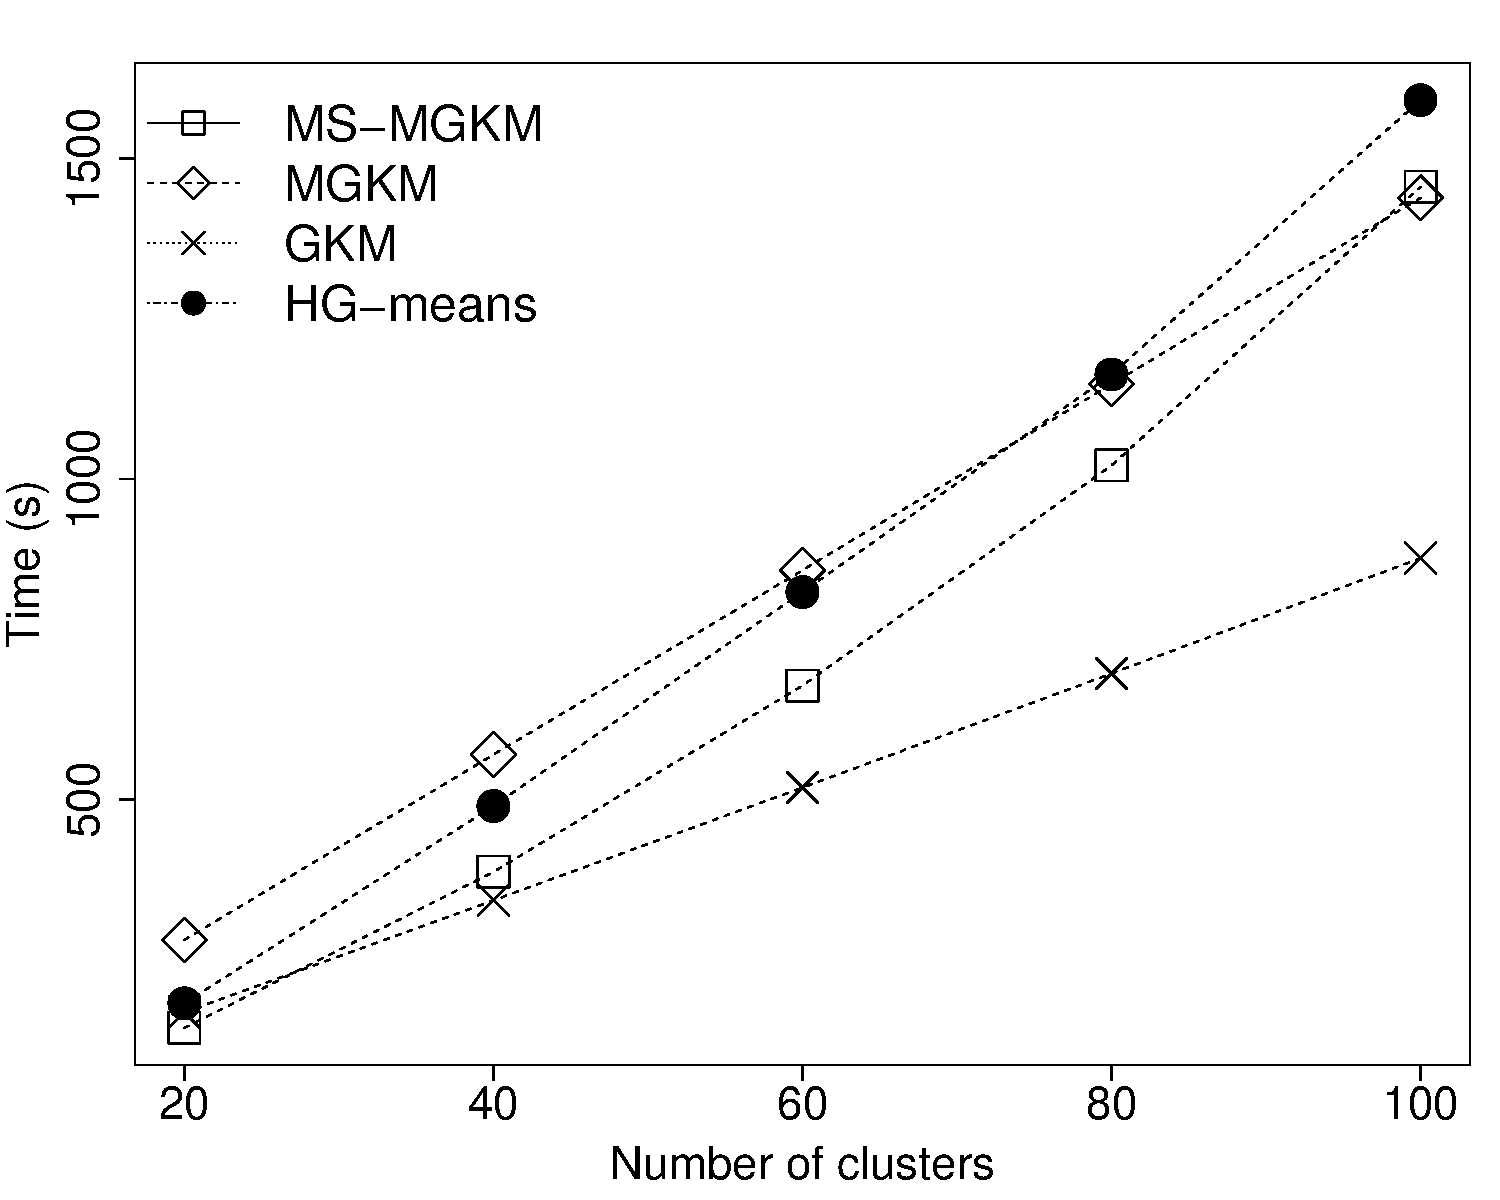
\includegraphics[width=0.48\textwidth]{img/cpu-pendigit}}
\subfigure[Letter ($n$ = 20000)]{\label{fig:time6}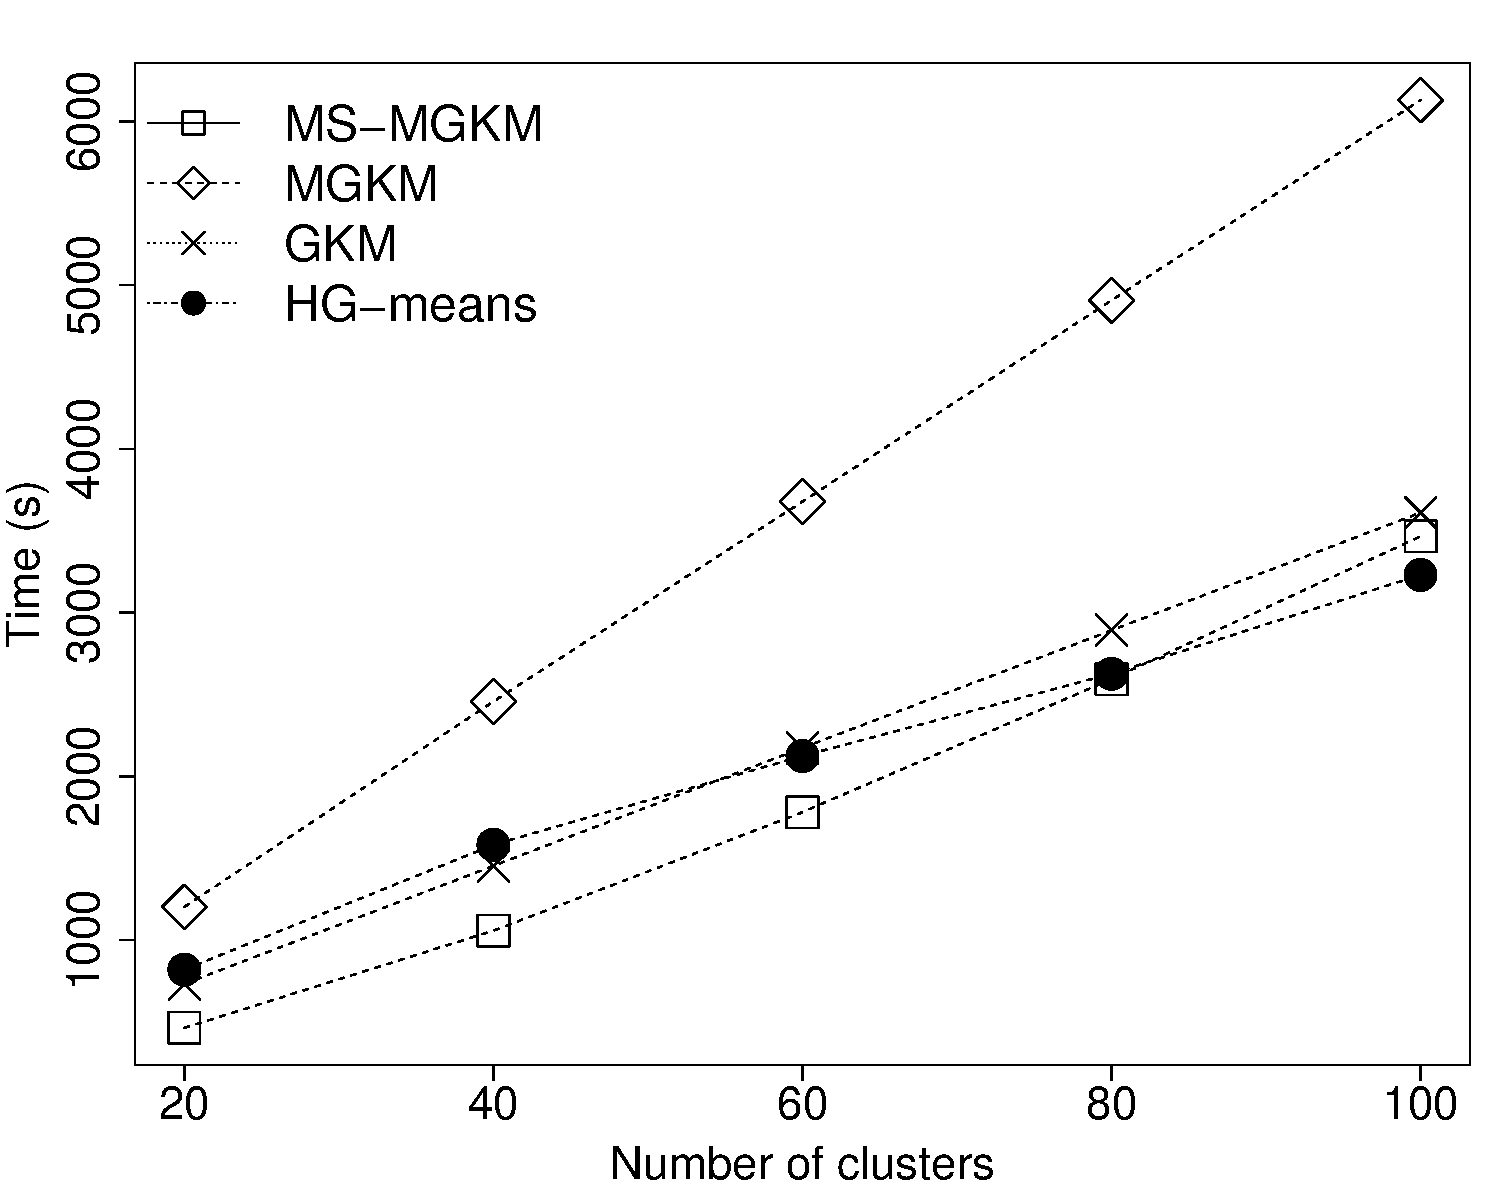
\includegraphics[width=0.48\textwidth]{img/cpu-letter}}
\caption{The CPU time of algorithms (Instances B)}
\label{fig:timeB}
\end{figure}

\begin{figure}[H]
\centering
\subfigure[Gas sensor ($n$ = 13910)]{\label{fig:time7}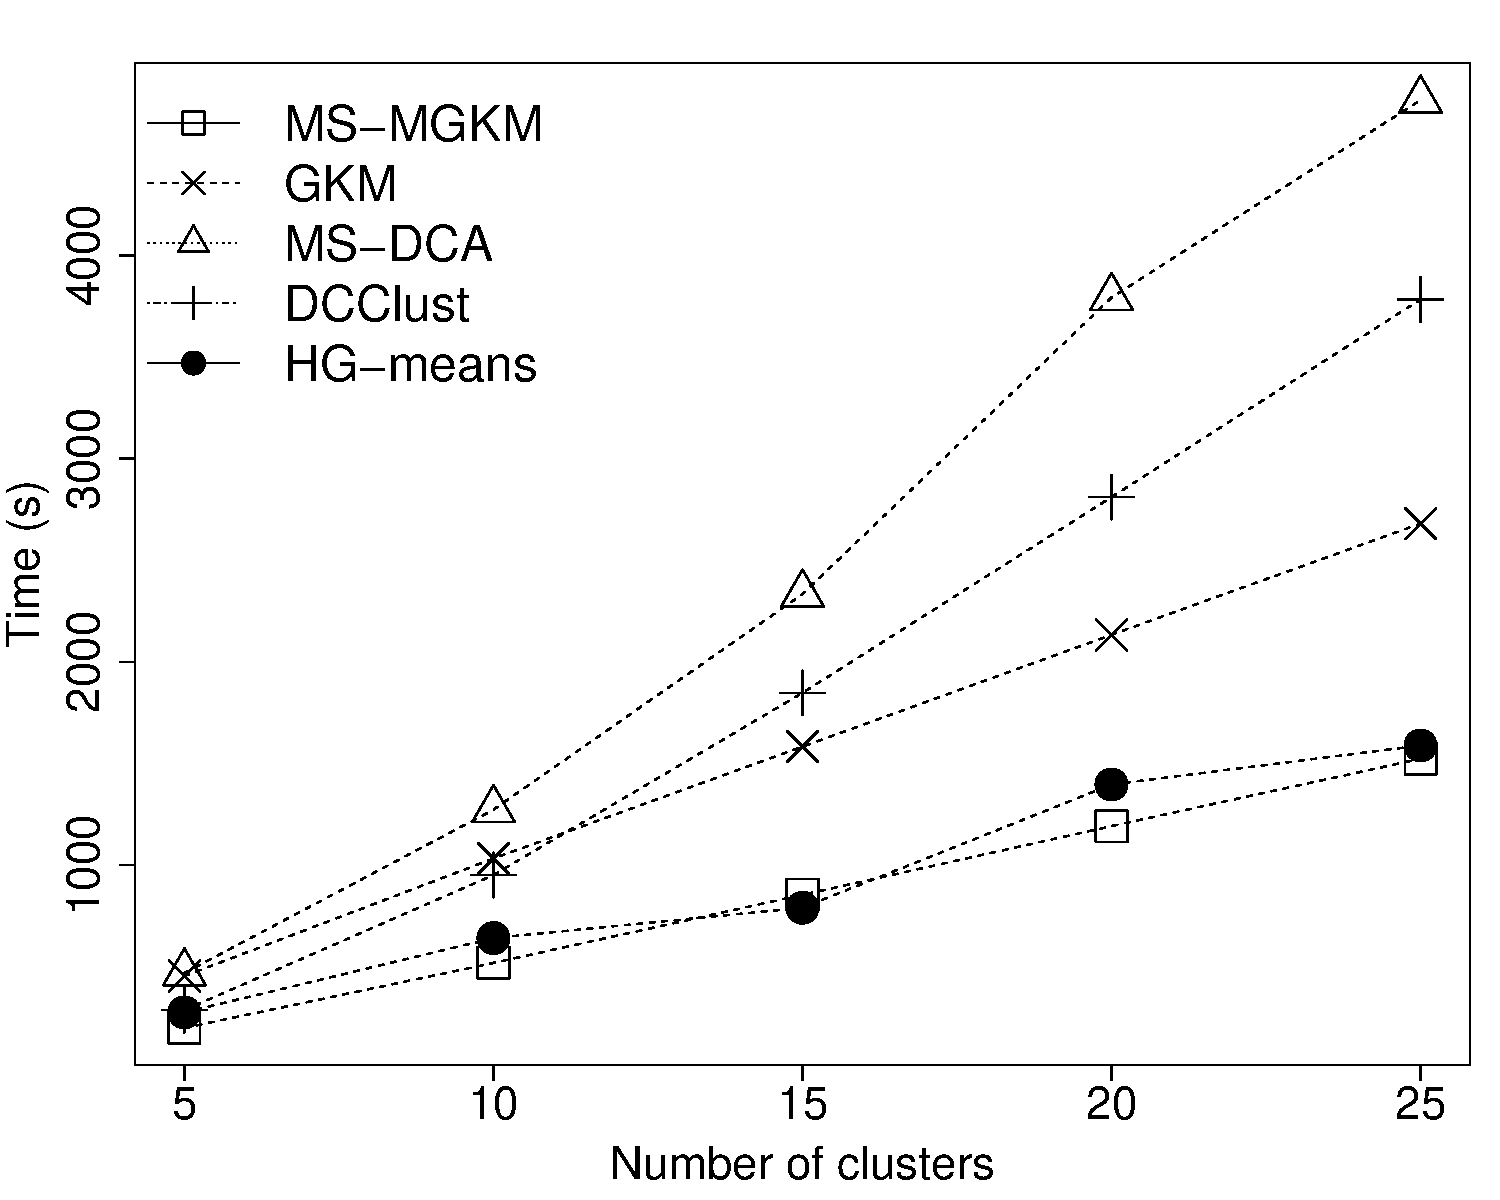
\includegraphics[width=0.45\textwidth]{img/cpu-gas}}
\subfigure[EEG eye state ($n$ = 14980)]{\label{fig:time8}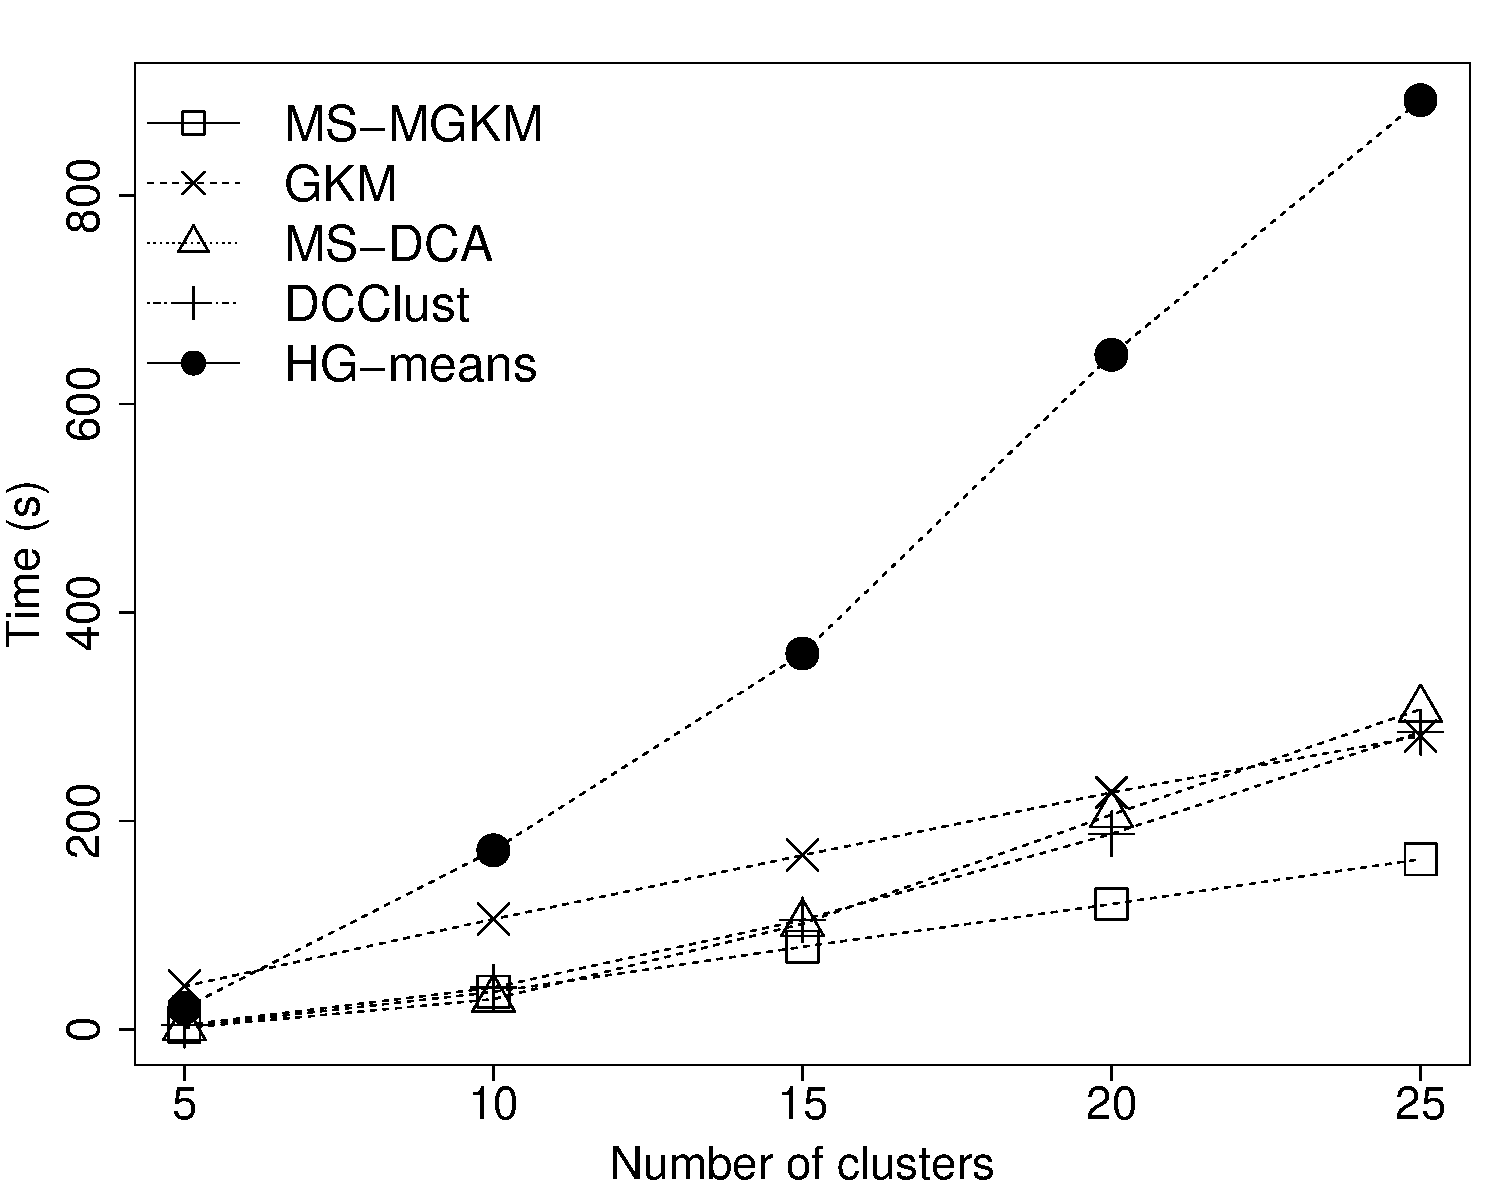
\includegraphics[width=0.45\textwidth]{img/cpu-eye}}
\subfigure[D15112 ($n$ = 15112)]{\label{fig:time9}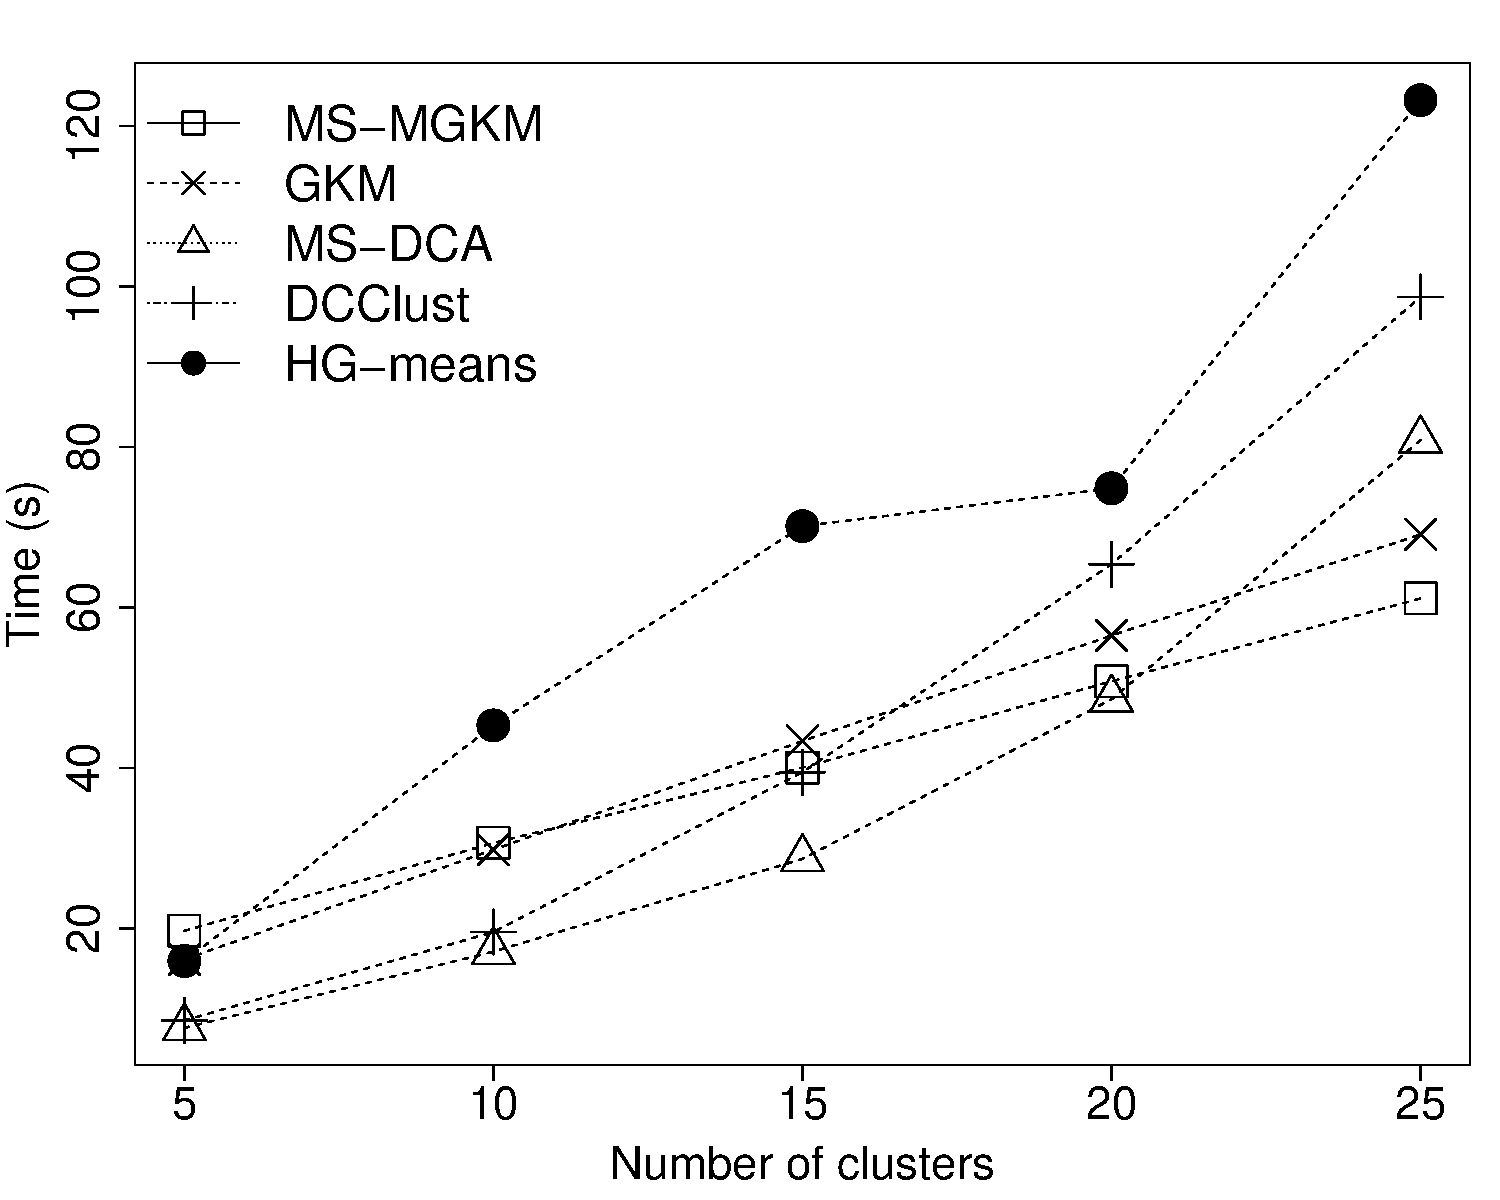
\includegraphics[width=0.45\textwidth]{img/cpu-d15112}}
\subfigure[KEGG metabolic ($n$ = 53413)]{\label{fig:time10}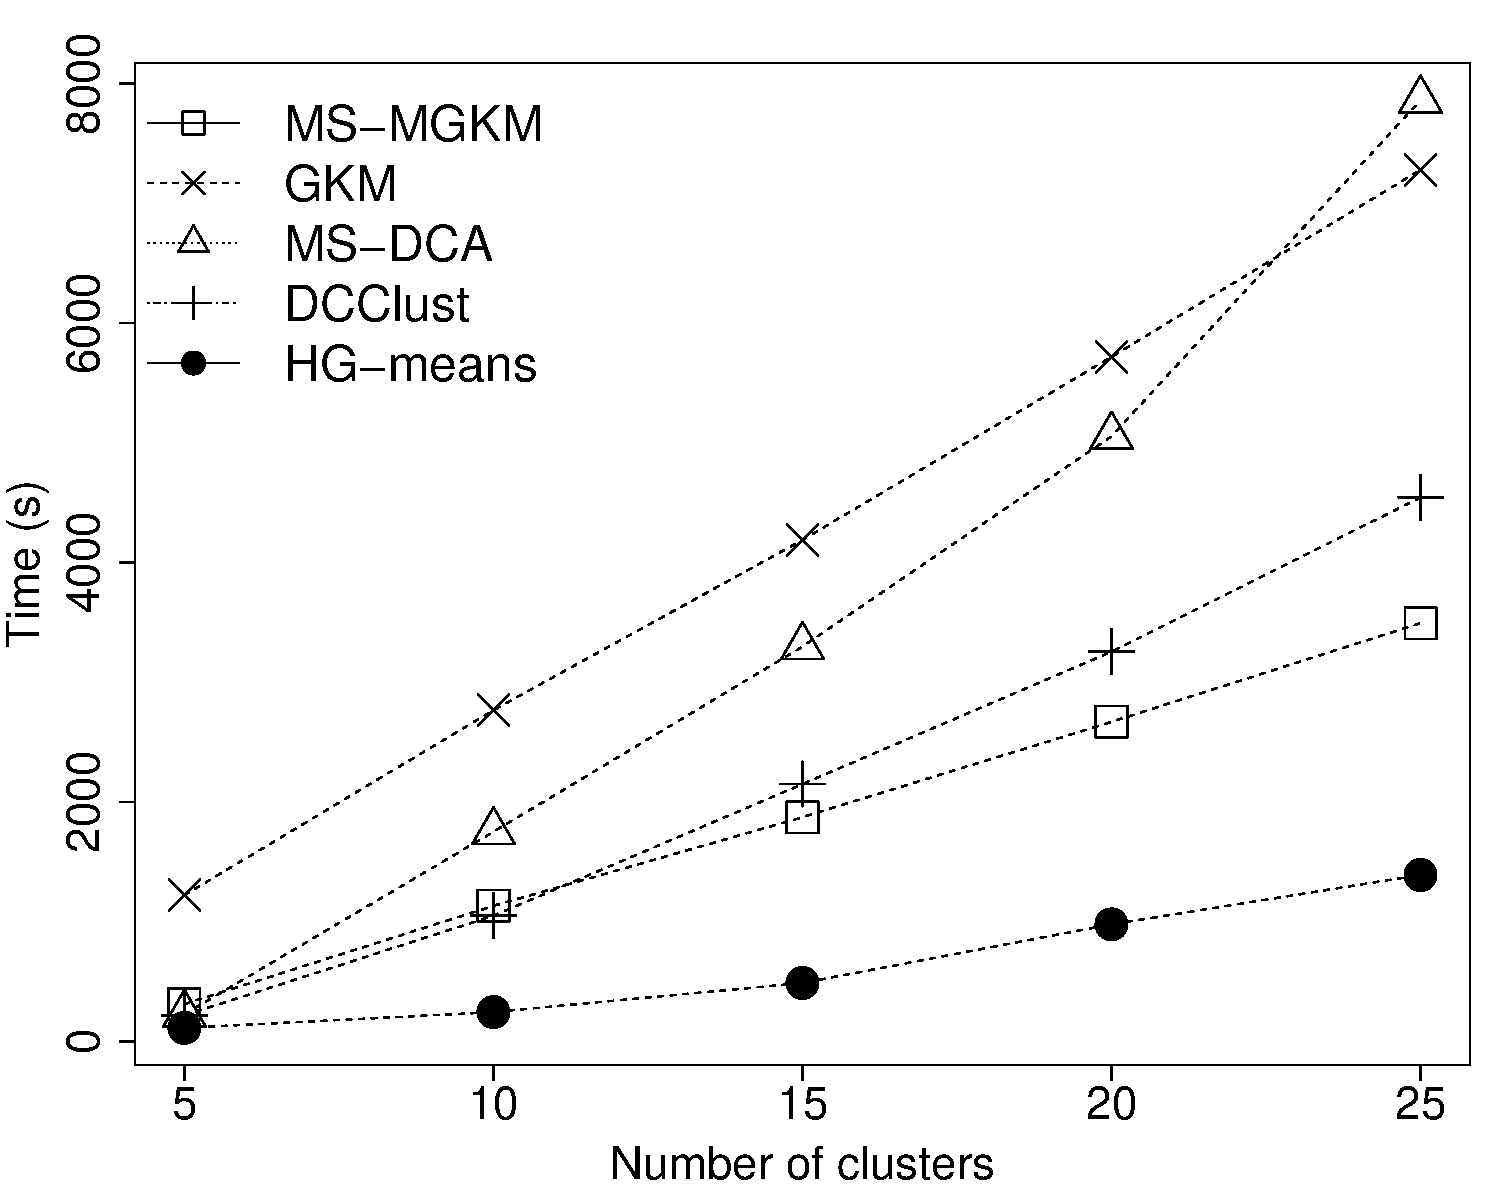
\includegraphics[width=0.45\textwidth]{img/cpu-kegg}}
\subfigure[Shuttle control ($n$ = 58000)]{\label{fig:time11}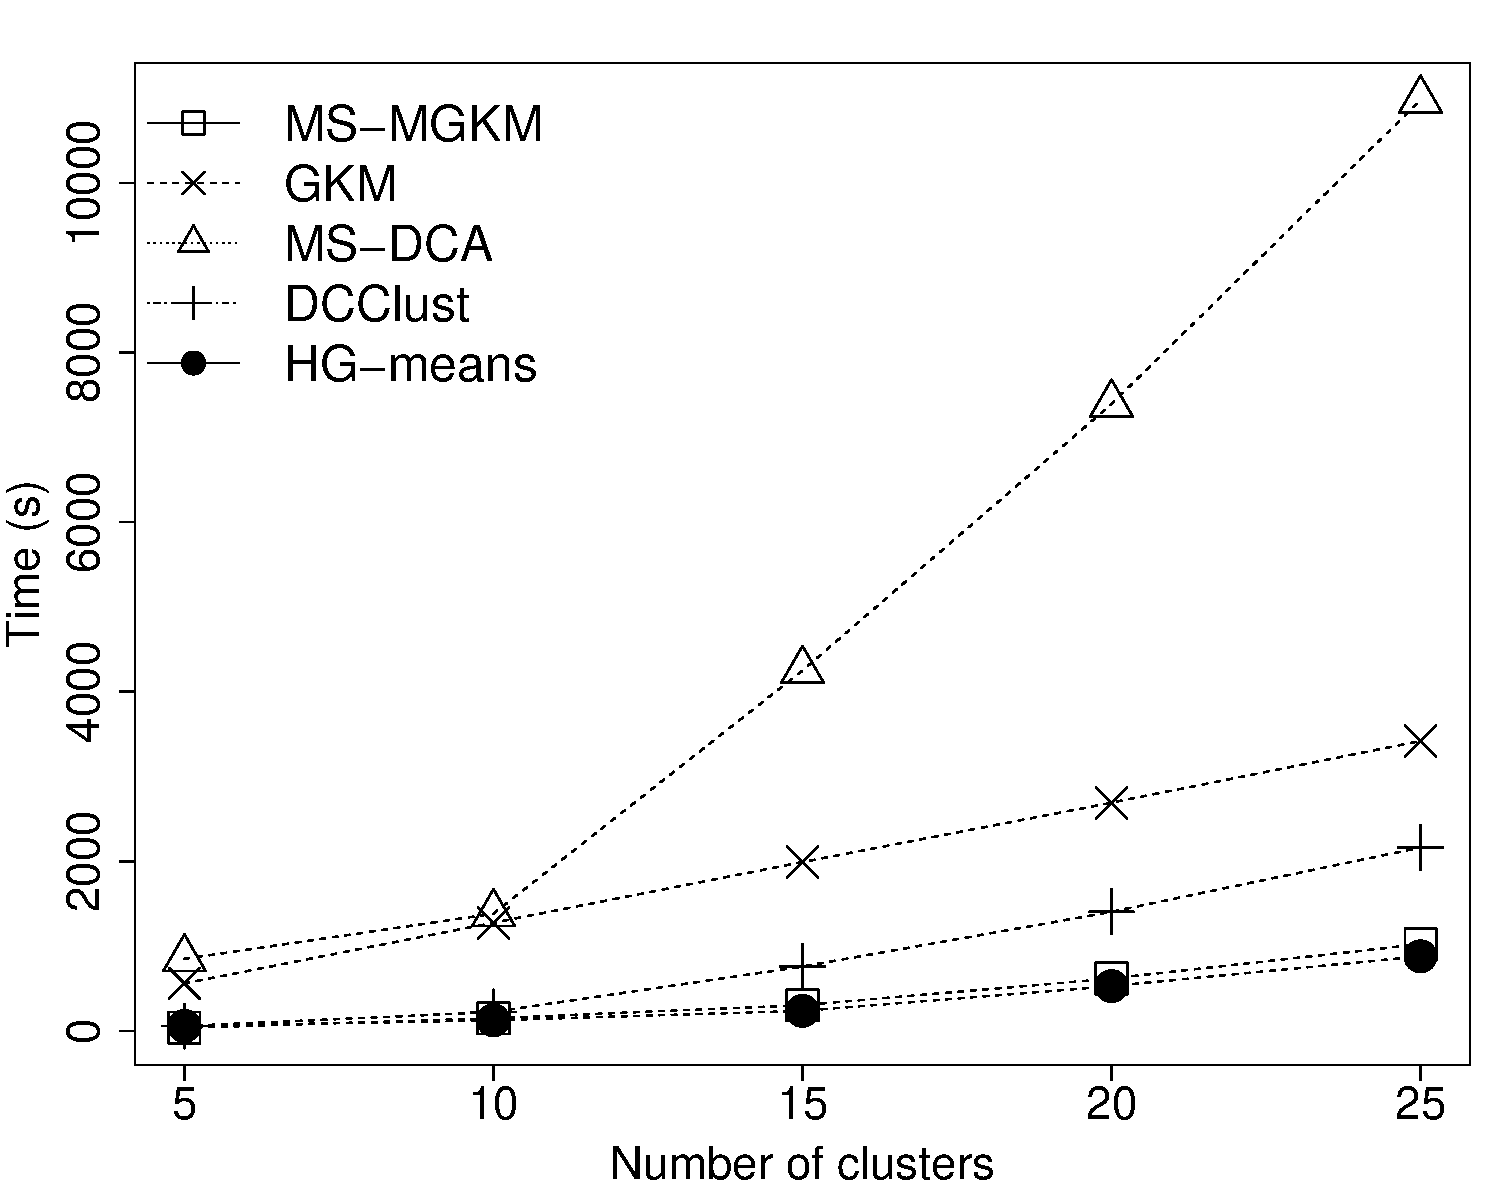
\includegraphics[width=0.45\textwidth]{img/cpu-shuttle}}
\subfigure[Pla85900 ($n$ = 85900)]{\label{fig:time12}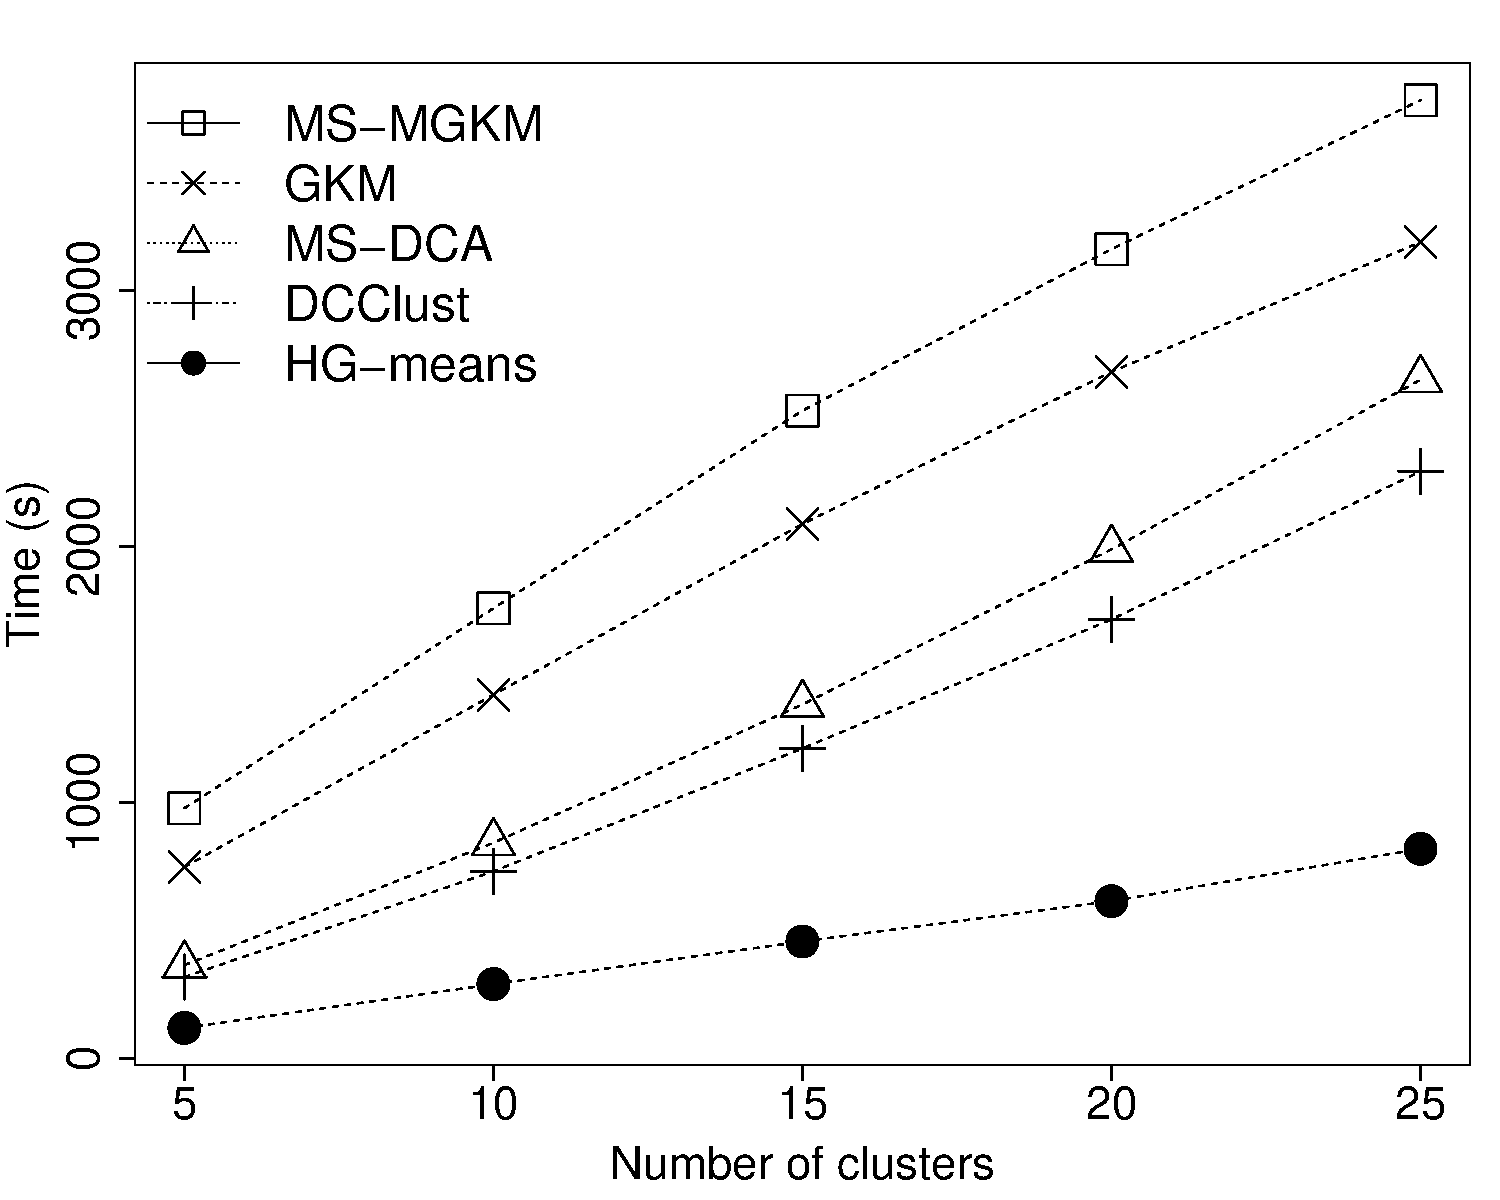
\includegraphics[width=0.45\textwidth]{img/cpu-pla85900}}
\subfigure[Skin segmentation ($n$ = 245057)]{\label{fig:time13}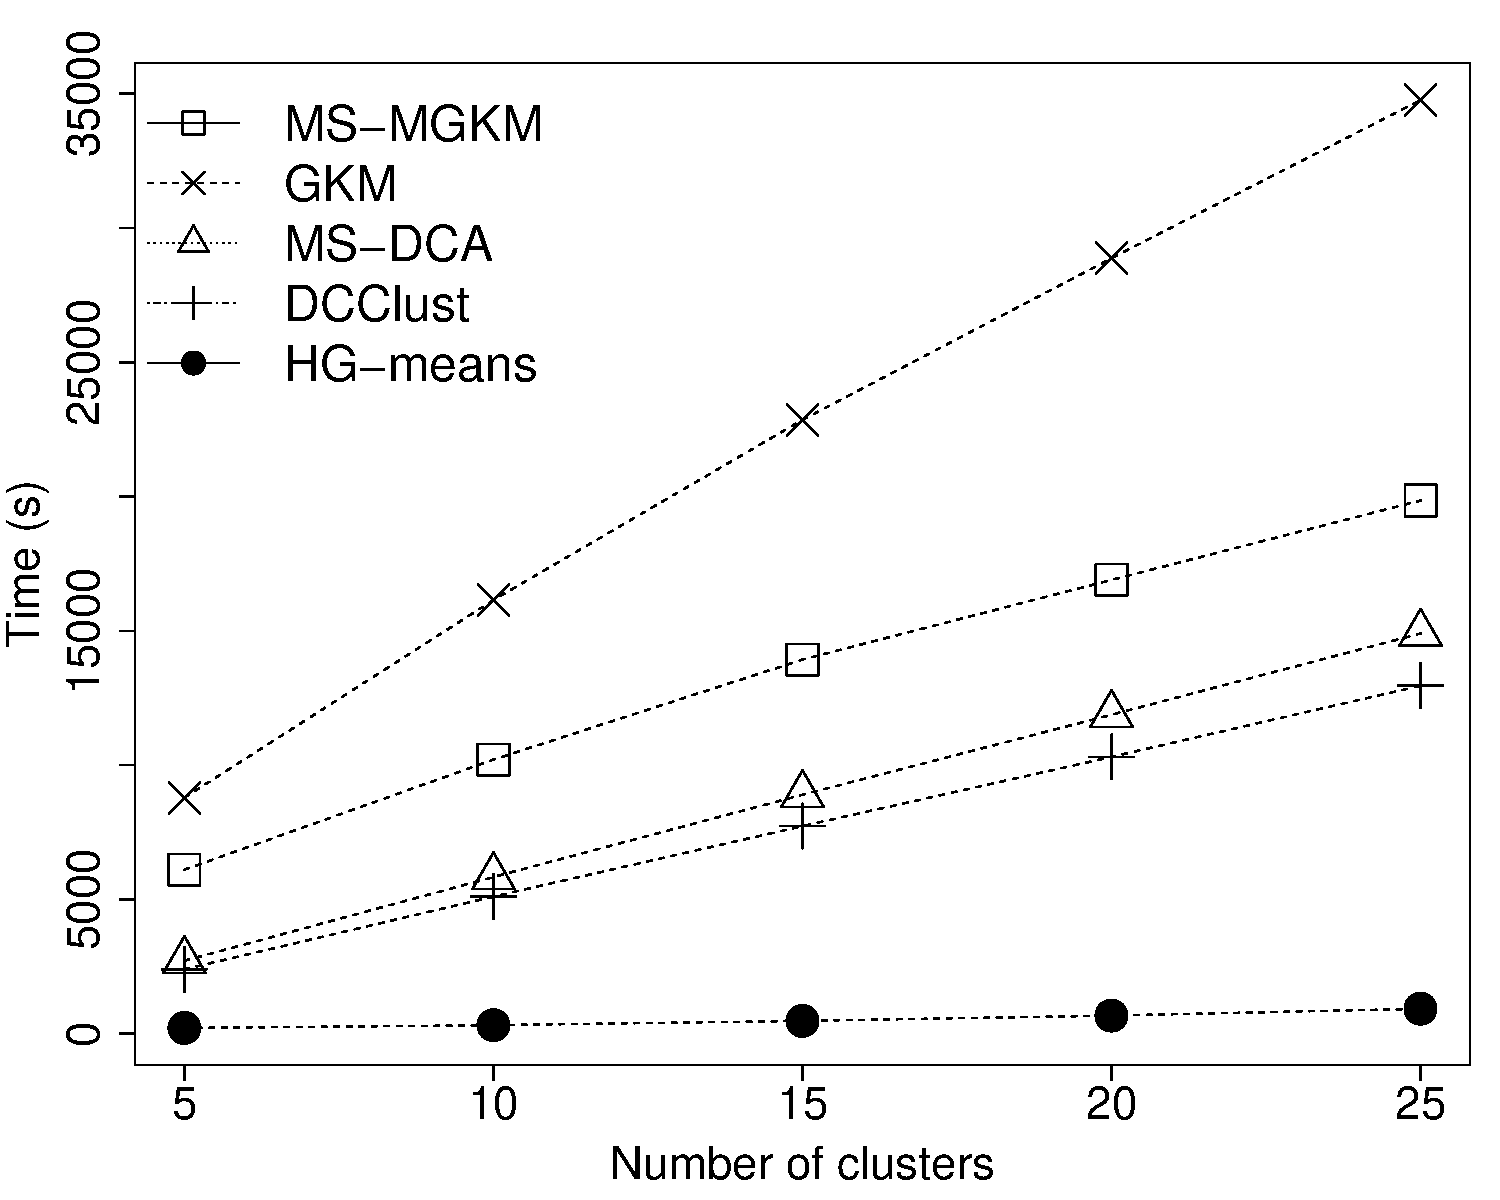
\includegraphics[width=0.45\textwidth]{img/cpu-skin}}
\subfigure[3D road network ($n$ = 434874)]{\label{fig:time14}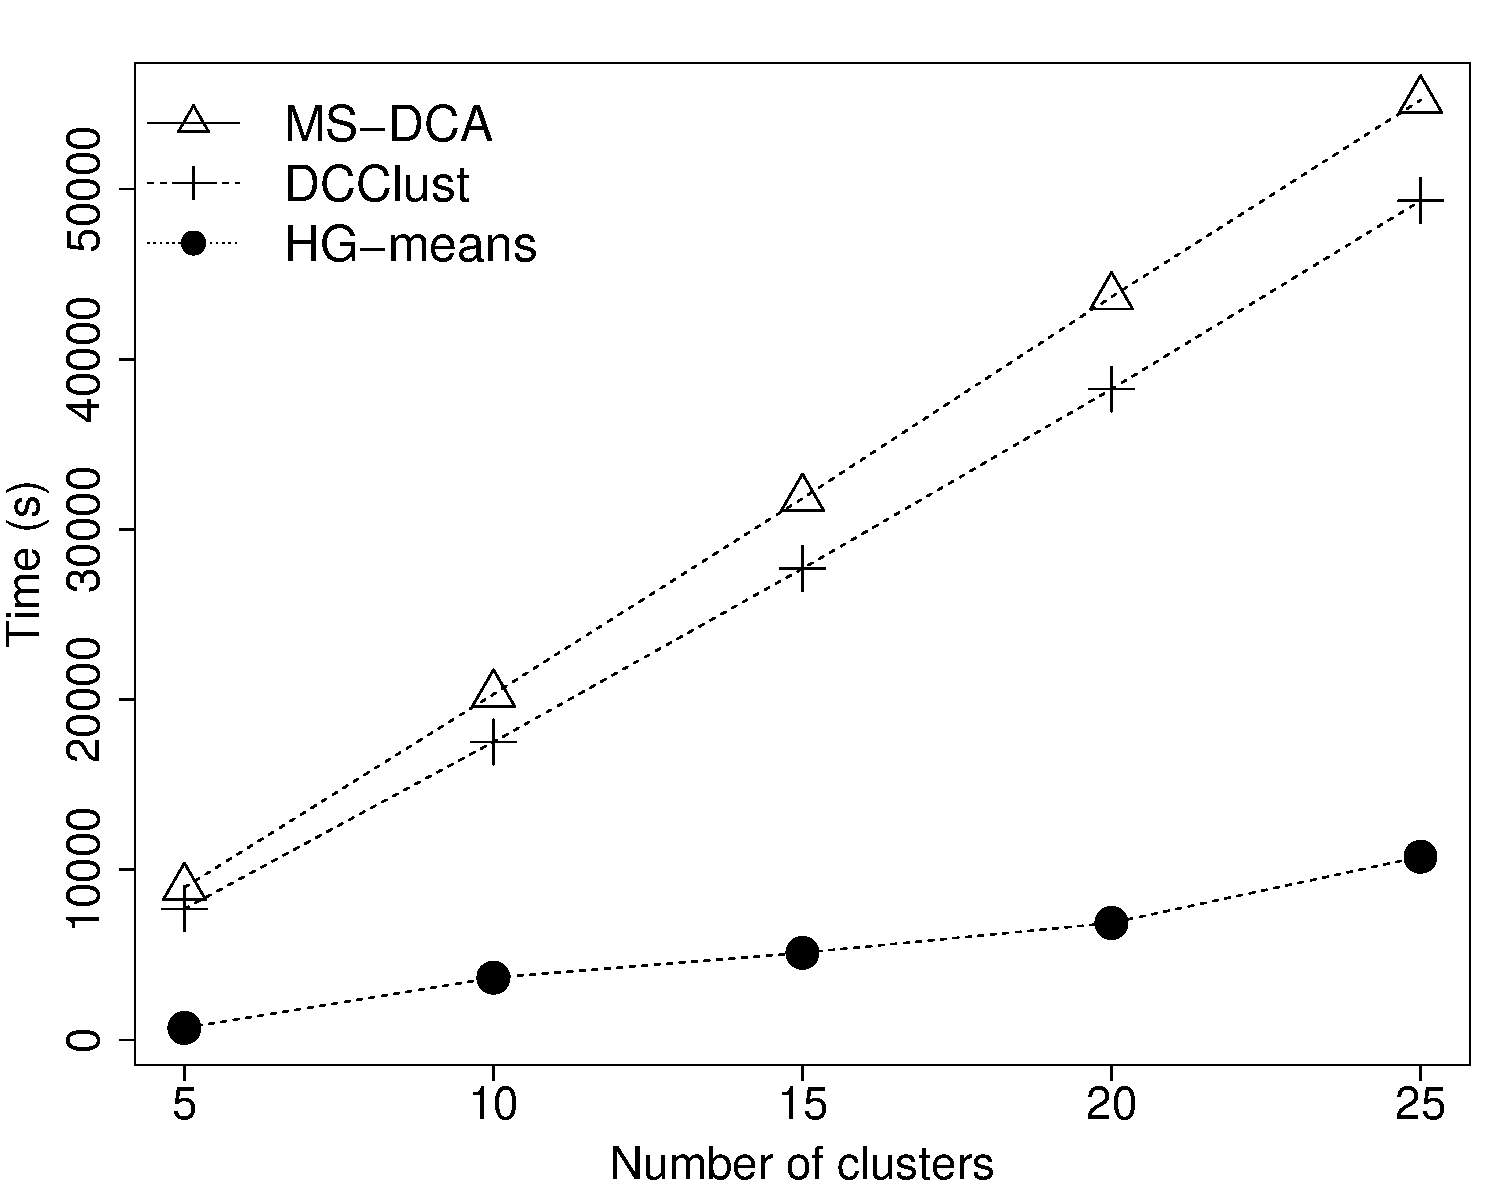
\includegraphics[width=0.45\textwidth]{img/cpu-3droad}}
\caption{The CPU time of algorithms (Instances C)}
\label{fig:timeC}
\end{figure}

\subsection{Components}
\label{sec:components-section}
In order to understand the contribution of components in the performance of HG-means, we performed some experiments by removing two important operators at a time: crossover and mutation. For comparison purposes, Table \ref{comp} reports the average error with respect to the best known solution in three scenarios: (i) complete HG-means with all components ($E_{avg}$), (ii) HG-means without mutation ($E_{avg}$ -M) and (iii) HG-means without crossover ($E_{avg}$ -C).

\small{\begin{table}[H]
%\small
\centering
\begin{tabular}{lccccccccc}
\hline
Instances A1 &      &       &        &        &        &       &       &       &       \\
m            & 2    & 3     & 4      & 5      & 6      & 7     & 8     & 9     & 10    \\
$E_{avg}$    & 0.00 & 0.00  & 0.00   & 0.00   & 0.00   & -0.01 & -0.17 & -0.03 & -0.06 \\
$E_{avg}$ -M & 1.94 & 32.57 & 117.64 & 118.07 & 158.28 & 34.66 & 54.85 & 80.79 & 95.18 \\
$E_{avg}$ -C & 0.00 & 0.00  & 0.00   & 0.00   & 0.00   & -0.01 & -0.17 & -0.03 & -0.06 \\ \hline
Instances A2 &      &       &        &        &        &       &       &       &       \\
m            & 2    & 5     & 10     & 15     & 20     & 25    & 30    & 40    & 50    \\
$E_{avg}$    & 0.00 & -0.02 & 0.94   & -0.82  & -1.26  & -1.48 & -1.51 & -1.64 & -1.78 \\
$E_{avg}$ -M & 0.00 & 0.45  & 3.67   & 3.75   & 5.20   & 6.21  & 6.03  & 4.80  & 3.93  \\
$E_{avg}$ -C & 0.00 & -0.02 & 0.95   & -0.61  & -0.85  & -0.82 & -0.59 & -0.26 & 0.26  \\ \hline
Instances B  &      &       &        &        &        &       &       &       &       \\
m            & 2    & 10    & 20     & 30     & 40     & 50    & 60    & 80    & 100   \\
$E_{avg}$    & 0.00 & -0.18 & -0.06  & -0.39  & -0.83  & -0.23 & -0.54 & -0.57 & -0.54 \\
$E_{avg}$ -M & 0.06 & 53.51 & 125.25 & 47.97  & 115.16 & 39.70 & 36.84 & 44.20 & 51.91 \\
$E_{avg}$ -C & 0.00 & -0.18 & -0.06  & -0.39  & -0.78  & -0.08 & -0.24 & 0.13  & 0.59  \\ \hline
\end{tabular}
\caption{HG-means performance in different scenarios: with all components, without mutation and without crossover}
\label{comp}
\end{table}}

Mutation and crossover are both essential to find high-quality solutions. For the case where we have HG-means without mutation, it does not find (in average) a solution better than the best known so far, while in the two other scenarios (complete HG-means and HG-means without crossover), it has a significantly better performance. Additionally, the complete HG-means algorithm performs better than the HG-means without crossover, especially when $m$ increases, indicating that the crossover is an essential operator when dealing with more complex clustering tasks.

%\noindent [TO-DO] analysis on number of features -- our algorithm seems to be fast when $d$ is small in small/medium instances (tsplib for example) but also when $d$ is large in large instances (gas sensor for example)